% !TEX root = ./main.tex

\documentclass{diploma} 

\usepackage{graphicx}
\usepackage{relsize}
\usepackage{booktabs}
\usepackage{color}
\usepackage{multirow}
\usepackage{bm}
\usepackage[percent]{overpic}
\usepackage{tcolorbox}

\usepackage{anyfontsize}
\usepackage{pgfplots}
\usepackage[normalem]{ulem}
\usepackage[dvipsnames]{xcolor}
\usepackage{colortbl}
\definecolor{cvprblue}{rgb}{0.21,0.49,0.74}
% \usepackage[pagebackref,breaklinks,colorlinks,allcolors=cvprblue]{hyperref}
\usepackage{tikz}

\def\mathdefault#1{#1}
\everymath=\expandafter{\the\everymath\displaystyle}
\pgfplotsset{compat=1.18}

\usetikzlibrary{calendar,fpu,matrix, positioning,arrows,arrows.meta,calc,decorations.pathreplacing,decorations.text,spy}
\tikzset{
  % style for inserting images as nodes
  img/.style={
      % text width=2cm, %% don't use this text height=2cm, %% don't use this
      inner sep=0pt,     % % use this
      outer sep=0pt,     % % and this
      rectangle,
      align=center} % only for debugging..
}

\newcommand{\KK}[1]{\textbf{\color{teal}[KK: #1]}}
\newcommand{\kk}[1]{{\color{teal}#1}}

\newcommand{\todo}[1]{{\color{red}#1}}  % a proposal text, use sparingly
\newcommand{\TODO}[1]{\textbf{\color{red}[TODO: #1]}}

\DeclareMathOperator*{\argmax}{arg\,max}
\DeclareMathOperator*{\mlp}{MLP}
\DeclareMathOperator*{\upsample}{upsample}
\DeclareMathOperator*{\downsample}{downsample}
\DeclareMathOperator*{\diag}{diag}
\DeclarePairedDelimiter\ceil{\lceil}{\rceil}
\DeclarePairedDelimiter\floor{\lfloor}{\rfloor}

% Support for easy cross-referencing
\usepackage[capitalize]{cleveref}
\crefname{section}{Sec.}{Secs.}
\Crefname{section}{Section}{Sections}
\Crefname{table}{Table}{Tables}
\crefname{table}{Tab.}{Tabs.}

\newcommand\mycoloredbox[1]{\textcolor{#1}{\rule{0.5em}{0.5em}}}
\definecolor{secondbestcolor}{HTML}{16E9CB}
\definecolor{firstbestcolor}{HTML}{169EE9}
\newcommand{\tablefirstbest}[0]{\cellcolor{firstbestcolor}}
\newcommand{\tablesecondbest}[0]{\cellcolor{secondbestcolor}}

\newsavebox\neuralnet
\begin{lrbox}{\neuralnet}
  \begin{tikzpicture}
    \node[circle, thick, fill=white, draw] (x1) {};
    \node[circle, thick, fill=white, draw, below=0.1em of x1] (x2) {};
    \node[circle, thick, fill=white, draw, below=0.1em of x2] (x3) {};
    \node[circle, thick, fill=white, draw, above=0.1em of x1] (x4) {};
    \node[circle, thick, fill=white, draw, above=0.1em of x4] (x5) {};

    \node[circle, thick, fill=white, draw, right=2em of x1] (x11) {};
    \node[circle, thick, fill=white, draw, below=0.1em of x11] (x12) {};
    \node[circle, thick, fill=white, draw, above=0.1em of x11] (x13) {};

    \foreach \x in {1,...,5}
    \foreach \y in {1,...,3}
    \draw (x\x) -- (x1\y);
  \end{tikzpicture}
\end{lrbox}

\usetikzlibrary{calendar,fpu,matrix, positioning,arrows,arrows.meta,calc,decorations.pathreplacing,decorations.text,spy}
\tikzset{
  % style for inserting images as nodes
  img/.style={
      % text width=2cm, %% don't use this text height=2cm, %% don't use this
      inner sep=0pt,     % % use this
      outer sep=0pt,     % % and this
      rectangle,
      align=center} % only for debugging..
}

\tikzset{
  moon colour/.style={
      moon fill/.style={
          fill=#1
        },
      scale=0.5,
    },
  sky colour/.style={
      sky draw/.style={
          draw=#1
        },
      sky fill/.style={
          fill=#1
        }
    },
  southern hemisphere/.style={
      rotate=180
    }
}

\makeatletter
\pgfcalendardatetojulian{2010-01-15}{\c@pgf@counta} % 2010-01-15 07:11 UTC --
% http://aa.usno.navy.mil/cgi-bin/aa_moonphases.pl?year=2010&ZZZ=END
\def\synodicmonth{29.530588853}
\newcommand{\moon}[2][]{
  {
      \tikzset{external/export=false}
      \edef\checkfordate{\noexpand\in@{-}{#2}}
      \checkfordate
      \ifin@
        \pgfcalendardatetojulian{#2}{\c@pgf@countb}% %
        \pgfkeys{/pgf/fpu=true,/pgf/fpu/output format=fixed}% %
        \pgfmathsetmacro\dayssincenewmoon{\the\c@pgf@countb-\the\c@pgf@counta-(7/24+11/(24*60))}% %
        \pgfmathsetmacro\lunarage{mod(\dayssincenewmoon,\synodicmonth)}
        \pgfkeys{/pgf/fpu=false}% %
      \else
        \def\lunarage{#2}
      \fi
      \pgfmathsetmacro\leftside{ifthenelse(\lunarage<=\synodicmonth/2,cos(360*(\lunarage/\synodicmonth)),1)}% %
      \pgfmathsetmacro\rightside{ifthenelse(\lunarage<=\synodicmonth/2,-1,-cos(360*(\lunarage/\synodicmonth))}% %%
      \tikz [moon colour=white,sky colour=black,#1]{
        \draw [moon fill, sky draw] (0,0) circle [radius=1ex];
        \draw [sky draw, sky fill] (0,1ex)
        arc (90:-90:\rightside ex and 1ex)
        arc (-90:90:\leftside ex and 1ex)
        -- cycle;
      }% %%
    }
}
\newcommand{\newmoon}{\moon{0}}
\newcommand{\waxingcrescent}{\moon{\synodicmonth/8}}
\newcommand{\firstquartermoon}{\moon{2*\synodicmonth/8}}
\newcommand{\waxinggibbous}{\moon{3*\synodicmonth/8}}
\newcommand{\fullmoon}{\moon{4*\synodicmonth/8}}
\newcommand{\waninggibbous}{\moon{5*\synodicmonth/8}}
\newcommand{\thirdquartermoon}{\moon{6*\synodicmonth/8}}
\newcommand{\waningcrescent}{\moon{7*\synodicmonth/8}}
\newcommand{\shadowed}{\moon{8}}
\newcommand{\unshadowed}{\moon{16}}
\newcommand{\removespace}[1]{\!\!\!\!\!\!\!\!\!\!#1\!}

\newcommand{\real}{\mathbb{R}}
\newcommand{\latentdimension}{D}
\newcommand{\projecteddimension}{d}

\makeatletter
\DeclareCiteCommand{\fullciteallauthors}
{\defcounter{maxnames}{99}
  \usebibmacro{prenote}}
{\usedriver
  {\DeclareNameAlias{sortname}{default}}
  {\thefield{entrytype}}}
{\multicitedelim}
{\usebibmacro{postnote}}

\renewcommand*{\mkbibnamegiven}[1]{
  \ifitemannotation{highlight}
  {\textbf{#1}}
  {#1}}

\renewcommand*{\mkbibnamefamily}[1]{
  \ifitemannotation{highlight}
  {\textbf{#1}}
  {#1}}

\makeatother
% \renewcommand{\paragraph}[1]{ \vspace{.5em}\noindent\textbf{#1} }

\newcommand{\conerf}{CoNeRF\xspace}
\newcommand{\blendfields}{BlendFields\xspace}
\newcommand{\lumigauss}{LumiGauss\xspace}
\newcommand{\clog}{CLoG\xspace}

% ======== CoNeRF ======= %

% % % basic math symbols %
\usepackage{dsfont}
\newcommand{\loss}[1]{\mathcal{L}_\text{#1}}
\newcommand{\calL}{\mathcal{L}}
\newcommand{\calN}{\mathcal{N}}
\newcommand{\calF}{\mathcal{F}}
\newcommand{\expect}{\mathbb{E}}
\newcommand{\IR}{{\mathbb{R}}}
\newcommand{\IE}{{\mathbb{E}}}
\newcommand{\balpha}{{\boldsymbol{\alpha}}}
\newcommand{\bbeta}{{\boldsymbol{\beta}}}
\newcommand{\bzero}{{\mathbf{0}}}
\newcommand{\bx}{{\mathbf{x}}}
\newcommand{\bc}{{\mathbf{c}}}
\newcommand{\bd}{{\mathbf{d}}}
\newcommand{\bC}{{\mathbf{C}}}
\newcommand{\boldm}{{\mathbf{m}}}
\newcommand{\bM}{{\mathbf{M}}}
\newcommand{\br}{{\mathbf{r}}}
\newcommand{\bv}{{\mathbf{v}}}
\newcommand{\bI}{{\mathbf{I}}}
\newcommand{\beps}{{\boldsymbol{\epsilon}}}
\newcommand{\Canonicalizer}{{\mathcal{K}}}
% \newcommand{\Canonicalizer}{{\mathcal{S}}}
% \newcommand{\LifterA}{{\mathcal{G}}} %< OBSOLETE
% \newcommand{\LifterB}{{\mathcal{H}}} %< OBSOLETE
\newcommand{\hypermap}{\mathcal{H}}
\newcommand{\Representation}{{\mathcal{R}}}
\newcommand{\Attribute}{{\mathcal{A}}}
\newcommand{\AttributeSet}{{\mathfrak{A}}}
\newcommand{\MaskSet}{{\mathfrak{M}}}
\newcommand{\reglambda}[1]{\lambda_\text{#1}}
\newcommand{\pars}{\boldsymbol{\theta}}
\newcommand{\given}{;}

\newcommand{\iImage}{c}
\newcommand{\nImages}{C}
\newcommand{\image}{\mathbf{C}}
\newcommand{\images}{\{\image_\iImage\}}
\newcommand{\latents}{\{\boldsymbol\beta_\iImage\}}
\newcommand{\latent}{\boldsymbol\beta}
\newcommand{\latentDim}{B}
\newcommand{\attrib}{\boldsymbol\alpha}
\newcommand{\allpars}{\boldsymbol\theta}
\newcommand{\iFrame}{k}
\newcommand{\width}{W}
\newcommand{\height}{H}
\newcommand{\nAttributes}{A}
\newcommand{\hyperAttributeDim}{d}
\newcommand{\iAttribute}{a}
\newcommand{\attribute}{\alpha}
\newcommand{\attributes}{\boldsymbol\alpha}
\newcommand{\Mask}{\mathbf{M}}
\newcommand{\mask}{\mathbf{m}}
\newcommand{\indicator}{\delta}
\newcommand{\gt}{\text{gt}}
\newcommand{\AttributeNet}{\mathcal{A}}
\newcommand{\point}{\mathbf{x}}
\newcommand{\MaskNet}{\mathcal{M}}
\newcommand{\stopgrad}{\xcancel{\nabla}}
\newcommand{\field}{\mathbf{f}}
\newcommand{\VolRend}{\mathcal{V}}
\newcommand{\ray}{\br}


\instytut{Faculty of Electronics and Information Technology}
\dyscyplina{Information and Communication Technology}
\title{Renderowanie Ludzi z Kilku Próbek z Użyciem Częściowej Informacji}
\engtitle{Few-Shot Human Neural Rendering with Partial Information}
% \album{KD-277}
\author{Kacper Kania, M.Sc.}
\promotor{Tomasz Trzciński, Prof. PhD DSc.}
\promotorpomocniczy{Marek Kowalski, PhD DSc.}
\date{2025}
\longdate{2025-01-01}
\thesisabstract{
  This thesis is a series of publications that introduce novel methods for human neural rendering using limited information, focusing on Neural Radiance Fields (NeRFs) and 3D Gaussian Splatting (3DGS).
  It explores how these models construct 3D representations from 2D images and
  demonstrates ways to condition these representations for generating
  high-quality human renderings.
  We propose techniques that use simple, interpretable inputs derived from
  sparse training data and extends these methods to perform effectively in
  few-shot learning scenarios.

  We begin by examining the field of neural radiance fields, addressing
  limitations in existing approaches and presenting contributions to
  controllable radiance fields.
  By incorporating partial and sparse data during training, it leverages the
  smoothness of neural networks to produce controllable, high-quality human
  images.

  To tackle the reliance on extensive, high-quality data annotations from
  multi-view videos, we introduce a new method for training neural radiance
  fields in few-shot, multi-view settings.
  This approach learns internal deformation templates, which blend smoothly
  during inference, significantly improving image quality compared to existing
  baselines and enabling effective human rendering from limited input images.

  The work also addresses the need for adaptable computational efficiency during
  inference.
  It proposes a fine-to-coarse learning strategy for 3D Gaussian Splatting,
  which upscales a latent 2D grid that stores Gaussian representations.
  This strategy achieves competitive results while allowing deployment on
  various computational devices with minimal quality loss.

  In addition, we develop a novel model for controlling radiance fields through
  environmental lighting.
  By incorporating precomputed radiance transfer, this model enables physically
  plausible scene relighting and provides users with intuitive control over
  lighting in reconstructed scenes.

  This research advances the state of the art in controllable neural radiance
  fields and expands their application to few-shot learning scenarios.
  These innovations enhance the possibilities for human rendering from limited
  information and open new directions for future research in the field.
}

\thesiskeywords{Neural Rendering, Neural Radiance Fields, Few-Shot Learning, Human Rendering, Partial Information, Gaussian Splatting}


\streszczeniepracy{
    To jest streszczenie. To jest trochę za krótkie, jako że powinno zająć całą stronę.
} % koniec streszczenia

\slowakluczowe{A, B, C}

\thesislaysummary{
  ok
}

\thesisacknowledgements{
    \lipsum[1-4]
} % end of abstract
\thesisarticles{
  \begin{table}[h]
    \resizebox{\linewidth}{!}{
      \begin{tabular}{cccc}
        \toprule
        \textbf{Title}                                                                                               & \textbf{Authors}                                                                                                                    & \textbf{Venue} & \textbf{Status} \\
        \midrule
        CoNeRF: Controllable Neural Radiance Fields                                                                  & \begin{tabular}{@{}c@{}}\textbf{Kacper Kania}, Kwang Moo Yi, \\Marek Kowalski, Tomasz Trzciński, \\Andrea Tagliasacchi\end{tabular}
                                                                                                                     & CVPR 2022                                                                                                                           & Accepted                         \\
        \midrule
        BlendFields: Few-Shot Example-Driven Facial Modeling                                                         & \begin{tabular}{@{}c@{}}\textbf{Kacper Kania}, Stephan J.
                                                                                                                         Garbin,   \\ Andrea Taglisacchi, Virginia Estellers, \\Kwang Moo Yi, Julien
                                                                                                                         Valentin, \\Tomasz Trzciński, Marek Kowalski\end{tabular}                                                         & CVPR 2023      &
        Accepted                                                                                                                                                                                                                                                                              \\

        \midrule
        \begin{tabular}{@{}c@{}}LumiGauss: High-Fidelity Outdoor Relighting with\\2D Gaussian Splatting\end{tabular} & \begin{tabular}{@{}c@{}}
                                                                                                                         Joanna Kaleta, \textbf{Kacper Kania}, \\ Tomasz Trzciński, Marek
                                                                                                                         Kowalski\end{tabular}                                                                    & WACV 2025      & Accepted                                                   \\
        \midrule
        CLoG: Leveraging UV Space for Continuous Levels of Detail                                                    & \begin{tabular}{@{}c@{}}
                                                                                                                         \textbf{Kacper Kania}, Rawal Khirodkar, \\Shunsuke Saito,  Kwang Moo Yi, \\Julieta Martinez\end{tabular}                            & CVPR 2025      & Under Review    \\
        \bottomrule

      \end{tabular} }
    % \caption{\textbf{Publications --} We present the list of publications that
    % are included in this thesis. We show the records in the chronological order,
    % together with their titles, authors, venues and status.
  \end{table}
}


\addbibresource{\jobname.bib}


\tikzexternalize


\begin{document}
\documentpreface{}
$\pi$
\hspace{1cm}
Stała matematyczna równa stosunkowi obwodu okręgu do jego średnicy

\ensuremath{I}
\hspace{1cm}
Natężenie prądu elektrycznego

% Akronim: nazwa symboliczna (dla LaTeXa), nazwa skrócona, nazwa pełna
\newacronym{IEEE}{IEEE}{Institute of Electrical and Electronics Engineers}
\newacronym{CPEE}{CPEE}{Computational Problems of Electrical Engineering}
\newacronym{PW}{PW}{Politechnika Warszawska}
\newacronym{IETiSIP}{IETiSIP}{Instytut Elektrotechniki Teoretycznej i Systemów Informacyjno-Pomiarowych}
\newacronym{laser}{LASER}{Light Amplification by Stimulated Emission of Radiation}

\newglossaryentry{symb:Phi}{
  name=$\phi$,
  description={foobar.},
  sort=symbolphi, type=symbols
}

\newglossaryentry{symb:I}{
  name={\ensuremath{I}},
  description={Natężęnie prądu elektrycznego.},
  sort=symbI, type=symbols
}

\newglossaryentry{symb:Pi}{
  name=$\pi$,
  description={Stała matematyczna równa stosunkowi długości okręgu do jego średnicy.},
  sort=symbolpi, type=symbols
}

\newglossaryentry{symb:rho}{
  name=$\rho$,
  description={Opór właściwy.},
  sort=symbolrho, type=symbols
}

\chapter{Introduction}
\label{chap:introduction}

                   With the advent of deep learning, research have been
                   exploring varying ways to apply it to computer graphics.
One of the most recent and promising approaches is neural rendering.
Neural rendering is a field that combines deep learning and computer graphics
to generate realistic images of 3D scenes.
The neural radiance field (NeRF) is a popular neural rendering technique that
represents a 3D scene as a continuous function that maps 3D coordinates to
radiance values.
NeRF has shown impressive results in generating photorealistic images of 3D
scenes.
However, NeRF has limitations in terms of memory and computational
requirements, which makes it difficult to scale to large scenes.

                   To alleviate the problem, \textcite{kerbl20233d} proposed a
                   new technique---3D Gaussian Splatting (3DGS).
3DGS is a neural rendering technique that represents a 3D scene as a set of 3D Gaussian that are splatted to an image space using algorithm proposed by~\textcite{zwicker2001ewa}.
 In contrast to NeRF, 3DGS is more memory efficient and can be used to render
 large scenes.
It can also render scenes with millions of points in real-time on a single
GPU.

                   In this thesis, we focus on those two milestone techniques
                   in neural rendering and address their fundamental
                   problem---lack of controllability.

\section{Motivation and challenges}

  NeRF and 3DGS are both impressive techniques that can generate realistic
  images.
  However, a single scene representation needs to be trained on a high-end GPU
  for hours or even days just to render a novel view at the inference time.
  However, any type of controllability is difficult to achieve with those
  models.
  That includes changing the lighting conditions, subject's attributes or even
  the scene itself.
  We see imbuing those models with controllability as a an important step
  towards making them more useful in practice.
  Our proposed models are designed to address this issue.

  One may ask why the controllability is a feat sought after to be researched.
  We see the inspiration in how human artists work.
  Imagine an artist working on 3D game where they need an asset, like a 3D
  mesh, to be created.
  Such a mesh takes much effort since it includes modeling, creating a UV map
  which can then be textured.
  After the process is finish, the artist's supervisor may task him to change
  the model to some extent which requires the artist to redo all the effort
  again.
  Such a process is not limited to 3D assets as meshes and could be applied to
  3DGS or NeRF.
  However, 3DGS and NeRFs are volumetric in nature.
  Our exploited and well-established practices no longer apply to them since
  volumetric representations do not have the underlying surface
  representation.
  For that reason, we see a couple of avenues which we explore in this thesis.

  Firstly, \textcite{park2021nerfies} proposed NeRFies, a model that creates a
  volumetric representation of a person from a self-captured sequence with a
  phone camera.
  Since the inception of NeRFs~\cite{mildenhall2020nerf}, it was among the
  first works the achieved such a high quality of reconstructions from a
  casual videos.
  In its primal form, NeRFies were unable to control the avatar in any other
  way than by a linear interpolation of latent embeddings that embedded the
  video's time dimension.
  The follow-up work, HyperNeRF~\cite{park2021hypernerf} handles this issue by
  projecting the learnable embeddings with $\latentdimension$ onto a
  lower-dimensional space~$\real^\projecteddimension$ where
  $\projecteddimension {\ll}\latentdimension$.
  After the assumption that the $\projecteddimension{=}2$ is enough to explain
  the sequence variability, that projected embedding becomes a 2-dimensional
  space that can be traversed in an interpretable way.
  However, that space is not intuitive since the projection is a non-linear
  operation and one cannot predict how values affect the results.
  To mitigate that issue, we propose to leverage smoothness of Multilayer
  Perceptrons (MLPs)~\cite{tancik2020fourier,park2021nerfies} to constrain the
  projection via sparse supervision.
  We realize our approach as a weakly-supervised MLP that out of many images
  from the sequence (we assume at least 100 frames in our work) only a few are
  provided with a coarse annotation.
  Such annotations denote what values a chosen attribute takes and where its
  effect spans in the image space.
  We show that our method, which we dubbed CoNeRF~\cite{kania2022conerf} and
  published at the CVPR 2022 conference, imbues NeRFs with a flexible
  editability feature without the lose of the rendering quality.

  Secondly, approaches such as CoNeRF~\cite{kania2022conerf},
  EditNeRF~\cite{liu2021editing} or FigNeRF~\cite{xie2021fig} focus solely on
  static elements of the scene, hence their controllability is limited to
  changing colors or textures in general.
  HyperNeRF~\cite{park2021hypernerf} arises as a potential solution due to its
  ability to model object deformations.
  However, our initial experiments showed that those changes cannot handle
  motions that affect a subject globally, \eg, jumping jacks performed by a
  person.
  To solve the issue, \textcite{fang2022fast} proposes to model the
  deformation via a multi-scale voxel structure which works well in the
  synthetic setting, such as the one proposed by~\textcite{pumarola2021d}.

  There exists a plethora of works that approach the problem from the another
  angle---instead of modeling the motion purely from data, they use a template
  model in the form of a 3D mesh to canonicalize deformed
  points~\cite{zielonka2022instant}.
  Such methods rely on the accuracy of the \textit{registration}, \ie, fitting
  the template mesh to subject.
  Since the registration methods~\cite{feng2021learning, zielonka2022towards}
  are imperfect estimators, they inherently contain registration errors.
  Those deviations are exacerbated by learnable radiance field models which
  assume a perfectly calibrated scene.
  The authors of those approaches usually mitigate the issue with additional
  latent space~\cite{grassal2022neural,kania2022conerf,martin2021nerfw} that
  requires thousands of video frames to learn an avatar of high-fidelity that
  reacts correctly to deformations such as wrinkles on the forehead.
  At the same time, performing the registration on the large scale is
  costly~\cite{cao2022authentic}.
  In this thesis, we seek a remedy for those obstacles.
  We propose a method that is data-efficient, easy to improve with a minimal
  user input and can model realistic deformation dependent changes in the
  subject.
  Inspired by classical methods in character texturing~\cite{oat2007animated}
  and motion modeling~\cite{lewis2014practice}, we propose
  BlendFields~\cite{kania2023blendfields}, an \textit{homage} to traditional
  blendshapes~\cite{lewis2014practice}.
  We build on VolTeMorph's~\cite{garbin2024voltemorph} approach to point
  canonicalization to provide a data-efficient way to control the character.
  We further introduce a physically-based mixture of predefined, learned from
  data wrinkle templates that represent expression-dependent skin
  deformations.
  Our proposed was acknowledged by the reviewers and was accepted to the CVPR
  2023 conference.

  Thirdly, having the texture and coarse mesh-based controllability, we strive
  for control scene settings directly.
  The inverse rendering of 3D scenes is an ill-posed problem where many
  different lighting settings may explain the same light
  effects~\cite{patow2003survey}.
  To facilitate solving the problem, many approaches use datasets of single
  object's images captured under different lighting
  conditions~\cite{chen2022hallucinated,yang2023crnerf,rudnev2022nerfosr}.
  These approaches cannot decouple albedo from the lighting
  effects~\cite{chen2022hallucinated,yang2023crnerf} or need additional neural
  networks to predict correct shadows~\cite{rudnev2022nerfosr} which limits
  methods' practicality.
  We propose to use recently proposed 2D Gaussian Splatting~\cite{huang20242d}
  which exhibit remarkable quality of the surface reconstruction.
  Together with our precomputed radiance transfer from classical computer
  graphics approaches~\cite{slomp2006gentle,ramamoorthi2001envmap}, our
  LumiGauss achieves state-of-the-art reconstruction quality with the ability
  to render novel lighting conditions with high fidelity.
  Our work received positive reviews for the WACV 2025 conference.

  Finally, volumetric representation are computationally intensive to render,
  compared to the traditional mesh representation.
  For NeRFs~\cite{mildenhall2020nerf}, it takes seven days on V100 NVidia GPU
  to train for single scene, and more than 60 seconds to render a single
  image---way beyond any practical applications.
  Although many approaches have been proposed to speed up the rendering
  process~\cite{garbin2021fastnerf,yu2021plenoctrees,reiser2021kilonerf,hedman2021baking,mueller2022instant},
  they usually make a trade-off between memory requirements, quality, and
  rendering speed.
  3D Gaussian Splatting~\cite{kerbl20233d} (3DGS) rose as an alternative to NeRF, offering both high-quality rendering at interactive frame rates.
  However, those frame rates could be achieved with the most advanced GPU
  units available at that time.
  As we see the potential in 3DGS to be a viable canonical representation for
  3D data, akin to 3D meshes, a need for its adaptability to different
  computational resources exists.
  Meshes can be adapted easily with levels of detail (LoD) approaches that
  remove detail from meshes that do not affect the general object's perception
  if necessary.

\section{Research objectives}
  In this thesis, we explore different avenues of radiance field
  controllability.
  With this goal in mind, we aim at answering the following research questions:
  \begin{enumerate}[label=(\textbf{RQ \arabic*})]
    \item \label{enum:texturing}
          Can we imbue a Neural Radiance Field (NeRF) with a controllability
          by providing sparse annotations to the training dataset?
          How many annotations suffice to learn smooth interpolation
          capabilities between controlled values?

    \item \label{enum:movement}
          Are extreme facial expressions known from the literature sufficient
          to learn expression-dependent details that extrapolate to
          expressions unseen at the training time?

    \item \label{enum:lighting}
          Is it possible to learn an underlying radiance transfer function of
          a scene from images taken in ``in-the-wild'' setting?
          Can such a transfer function generalize to unknown environment maps?

    \item \label{enum:resources}
          How to learn a single 3D Gaussian Splatting (3DGS) representation
          that can be adapted to different computational regimes at inference
          time in a feed-forward mode?
  \end{enumerate}

  Each of these questions is a representative of possible among many others
  controllability directions for radiance fields.
  In case of this thesis, we present summarize our methods as controls of:
  texture~\cite{kania2022conerf,kania2023blendfields},
  shape~\cite{kania2023blendfields}, lightning~\cite{kaleta2024lumigauss} and
  use of resources~\cite{kania2024clog}.
  To answer~\ref{enum:texturing}, we describe our
  CoNeRF~\cite{kania2022conerf}.
  It is one of the pioneering works that uses sparsely annotated frames to
  continuously control the subject in a post-hoc manner.
  We leverage the fact that MLP used in NeRFs are smooth functions biased
  towards low frequency signals~\cite{tancik2020fourier}.
  For that reason, NeRF can learn to interpolate smoothly the annotation
  signal between frames of high similarity.
  We show that this assumption is sufficient to obtain both novel view
  synthesis and novel attribute synthesis with a single model.

  We further move towards answering~\ref{enum:movement}.
  We introduce BlendFields~\cite{kania2023blendfields}, achieving two primary
  goals: ability to generalize unknown expressions via a predefined face mesh
  template, and a mixture model of training expressions that can produce
  spatially coherent, expression-dependent wrinkles on the face from as few as
  three expressions.
  In our work, we build on VolTeMorph~\cite{garbin2024voltemorph} to achieve
  to former, and focus on the latter contribution.
  Inspired by texture maps in classical computer graphics
  pipelines~\cite{oat2007animated}, we define a set of learnable radiance
  fields, each being overfit to a particular extreme expression from the
  training set.
  We define an extreme expression as one of the possible expressions involving
  the most facial muscles.
  Building on VolTeMorph~\cite{garbin2024voltemorph} allows us to use an
  underlying tetrahedral mesh to compute physical quantities such as the
  volume change of tetrahedra under a given expression.
  We use those quantities to linearly interpolate between the pretrained
  radiance fields.
  We mix the tetrahedra independently which makes rendering novel expressions
  possible.
  For example, BlendFields can render one of the eyebrows raised while
  maintaining the other in a natural position, which is a difficult expression
  to make for majority of people.

  Our LumiGauss~\cite{kaleta2024lumigauss} answers~\ref{enum:lighting}.
  In contrary to common approaches~\cite{rudnev2022nerfosr}, we posit that the
  radiance transfer function known among computer graphics
  researchers~\cite{ramamoorthi2001envmap} can be learned from unconstrained
  photo collection under varying lighting conditions.
  To this end, we use 2DGS~\cite{huang20242d} which gives us a smooth shape
  representation, difficult to achieve when using 3DGS~\cite{kerbl20233d}.
  With the use of contributed priors, we induce learning Gaussian's Spherical
  Harmonics such that they correctly react to changing environment maps.
  Not only our approach is fast to train, but renders realistic scenes and
  object's shadows even under novel lighting conditions.

  All the contributions so far are affected by a specific disadvantage---a
  single model needs to be trained from scratch and it can be deployed only on
  high-end hardware.
  We then ask if we can train a single model that is adaptable at inference
  time to different hardware regimes~\ref{enum:resources}.
  We propose CLoG~\cite{kania2024clog} as a potential remedy.
  Our approach uses the fact that one can constrain the number of Gaussians in
  3DGS~\cite{kerbl20233d} to a specific number, such that it can be formed as
  a 2D grid by simple reshape operation.
  With a specific training coarse-to-fine training protocol we contributed,
  the model learns a representation that converges to a high-quality
  volumetric structure.
  In the second training stage, we leverage the fact that Gaussians's can be
  spatially sorted in such a manner that their descriptors are placed next to
  each other if they are similar.
  That forms a low-frequency image which can be modulated with an
  off-the-shelf continuous upsampling architecture~\cite{vasconcelos2023cuf}.
  The architecture outputs a new grid of the given resolution.
  We show in our work that such an approach achieves remarkable results and
  can output any number of Gaussians at inference time with high quality.

\section{Contributions}
  Building on those questions, we structure this thesis in several chapters
  corresponding to the answers.
  An answer is in a form of a scientific article where we introduce the following:
  \begin{itemize}
    \item A novel approach for controlling trained radiance fields with the use of sparsely annotated images from a casually captured data.
    \item A new model capable of blending trained radiance fields from multi-view frames in an interpretable way and extrapolating to novel human expressions for the trained subject.
    \item The first use of Gaussian Splatting methods that learns a coherent shape representation of a subject and an ability to distill the varying lighting conditions in the data to a radiance transfer function.
    \item A novel paradigm for learning Gaussian Splatting models as 2D grids to achieve flexibility to adapt the model to different computational regimes at inference time.
  \end{itemize}

  % not using primes (not canonicalized parameters)
\begin{figure}
  \centering
  \begin{subfigure}[t]{0.38\linewidth}
    \centering
    \includegraphics[width=\linewidth]{assets/conerf/img/beta-importance-annotations.pdf}
    \caption{annotated samples}
  \end{subfigure}
  \hfill{}
  \begin{subfigure}[t]{0.595\linewidth}
    \centering
    \includegraphics[width=\linewidth]{assets/conerf/img/beta-importance-preds.pdf}
    \caption{renderings from the trained model}
  \end{subfigure}
  \caption{{\bf Example with annotations and controlled attributes --}
    We show an example of how our \conerf is capable of controlling attributes
    selected sparse annotations at the training time.
    Top row shows possible value combinations ($\color{red}{-}$ denoting closed
    eye, $\color{orange}{0}$ neutral position and $\color{green}{+}$ an open eye)
    and $\{\bbeta_1,\bbeta_2\}$ possible values of attributes that are not
    explicitly learned from the annotations but purely from data (please
    see~\cref{chap:conerf} for further explanation).
  }
  \label{fig:conerf-teaser}
\end{figure}
  \subsection{Texture from Partial Information}
    Existing NeRF-based approaches in 2021 were simple models---they were
    overfit to a single subject, for a new subject the model needed to be
    retrained from scratch, and the editability capabilities were
    limited~\cite{liu2021editing}.
    NeRFactor~\cite{zhang2021nerfactor} could be considered a more
    sophisticated model.
    However, it worked only for simple scene with calibrated scenes and could
    not handle any motion.

    We approach those issues in our CoNeRF~\cite{kania2022conerf} published at
    the CVPR 2021 conference.
    Inspired by HyperNeRF~\cite{park2021hypernerf}, we propose to revisit the
    weak supervision in the context of radiance fields.
    Specifically, under an assumption that one can provide a few of sparse
    annotations to the dataset, we can leverage the smoothness of the neural
    networks to propagate the annotation across the dataset.
    The annotations also consist of what regions in the image space it refers
    to and hence we can train a semantic segmentation radiance fields that
    decouples attribute controls.
    We show an example in~\cref{fig:early-conerf-teaser-intro} where the left
    side represents the annotations present in the data and the right one
    possible manipulations at the inference time.
    We note that those annotations are easy to make in a matter of a few
    minutes for a single dataset.
    However, the complexity of the annotations grows with the number of
    attributes to control.

  \subsection{Expression from Few-Shot Learning}
    \conerf~\cite{kania2022conerf} is capable of rendering complex motions
    given sufficient amount of data and provided annotations.
    However, motions as the ones a person performs daily when speaking are
    infeasible in practice.
    We propose a solution to target that issue.
    We introduce \blendfields~\cite{kania2023blendfields} from the CVPR 2023
    proceedings which learns motion-dependent face deformation from data.
    We build on VolTeMorph~\cite{garbin2024voltemorph} which uses existing
    face template models, such as FLAME~\cite{li2017flame}, to learn a single
    canonical representation, akin to the canonicalization module in CoNeRF.
    Internally, \blendfields creates a tetrahedral cage around the face model.
    For each sample along the ray in NeRF, it moves the points to a ``neutral
    position'', chosen once prior to the training procedure.
    Such a procedure comes insufficient to model realistic facial features,
    such as wrinkles.
    We contribute a novel approach to modeling those deformations.
    We compute a deformation gradient of each tetrahedra for a given
    expression which is a physically-based and easy to interpret quantity.
    The value serves us to smoothly transition face regions textures to
    appropriate colors.
    We obtain the colors from NeRFs branches, each overfit to particular
    expression.
    In principle, \blendfields predicts face bases which are conditioned on
    the face expression vector to output the final point color.
    Our framework works well even when only a few ``extreme'' expressions are
    provided such as grinning face with closed eyes and wide open mouth with
    open eyes.

  \subsection{Light from Unconstrained Images}
    In both approaches above, we tackle the problem of texture
    controllability.
    They assume an ideal case scenario where a capture can be taken in an
    idealized environment with constant camera exposure and lighting.
    Moreover, the produced colors are blended together, making the change of
    light impossible in practice.
    We then ask the questions if we can decouple an intrinsic color of the
    subject and change of that color stemming from the environment light.
    We answer that question with our \lumigauss~\cite{kaleta2024lumigauss}
    published at the WACV 2025 conference that, indeed, we can achieve that by
    learning the radiance transfer function directly from data.
    For that end, we train a 2DGS~\cite{huang20242d} model to obtain a smooth
    and spatially coherent surface of objects.
    On top of the other attributes known from 3DGS~\cite{kerbl20233d}, we
    imbue our Gaussians with additional features corresponding to the radiance
    transfer, expressed as Spherical Harmonics~\cite{green2003grittydetail}.
    We show in our experiments that such a formulation is sufficient to train
    a model that reacts to changing environment maps in a realistic manner and
    renders images of higher fidelity than prior approaches.

  \subsection{Levels of Detail in One Model}
    All the contributions above require considerable computation hardware to
    be trained on and then run inference in near real-time frame rates.
    Drawing an inspiration from the gaming industry where Levels of Details
    (LoD) for meshes is used heavily, we introduce \clog~\cite{kania2024clog}.
    Our approach trains a single Gaussian Splatting model such that it can be
    modulated at inference time and adapted to the target computational
    requirements with a minimal loss on the rendering quality.
    That allows us to democratize the use of 3DGS and deploy a single model
    even on handheld devices.
    We show later that even under a strict case where only 2,000
    Gaussians\footnote{Common 3DGS models can achieve from $10^5$ to even
    $10^6$ Gaussians.
    } can be used, the object is still recognizable.
    The most important contribution of our model is that it is continuous by
    design while the existing baselines assume prior the training the model
    how many LoD the model should comprise at inference.
    To change the size of particular LoD in those baselines requires training
    the whole model from scratch, imposing a significant computational burden.

\section{Thesis outline}
  This thesis is structured as follows.
  We start by introducing the preliminaries related to the Neural Radiance
  Fields and Gaussian Splatting in~\cref{chap:background}---a common theme in
  all works that appear later.
  We then move towards describing CoNeRF~\cite{kania2022conerf}
  in~\cref{chap:conerf}, our approach to control trained neural radiance
  fields by using sparse annotations.
  In~\cref{chap:blendfields}, we describe
  BlendFields~\cite{kania2023blendfields} that can produce realistic
  expression-dependent texture from just a few multi-view frames of the
  subjects.
  \cref{chap:lumigauss} introduces the LumiGauss~\cite{kaleta2024lumigauss}, a Gaussian Splatting model that learns a radiance transfer function for novel lighting rendering capabilities.
  Finally, we bring a general method, CLoG~\cite{kania2024clog}, that uses
  Gaussian Splatting to learn continuous levels of detail while training only
  a single model.
  We conclude the thesis in~\cref{chap:final} where we also explore possible
  future avenues that can be undertaken.

\section{Publications not included in the thesis}
  We attach a list of articles that are related to and can be used to in neural rendering approaches:
  \begin{itemize}
    \item\!\!\!\fullciteallauthors{kania2020ucsg},
    \item\!\!\!\fullciteallauthors{kania2021trajevae},
    \item\!\!\!\!\!\fullciteallauthors{stypulkowski2021representing},
    \item\!\!\!\!\fullciteallauthors{xia2023densify},
    \item\!\!\!\fullciteallauthors{esposito2024geogen},
    \item\!\!\!\!\fullciteallauthors{spurek2024modeling}.
  \end{itemize}


\chapter{Background}
\label{chap:background}

\section{Neural Rendering}
\section{Neural Radiance Field}
\section{3D Gaussian Splatting}
\chapter{CoNeRF: Controllable Neural Radiance Fields}
\label{chap:conerf}
\newcommand{\conerfdirname}{3_conerf}
\newcommand{\teasernobox}{
  \begingroup
  \begin{subfigure}[b]{0.170\linewidth}
    \centering
    \includegraphics[width=\linewidth]{fig/\conerfdirname/assets/teaser/annotations.pdf}
    \subcaption{annotations}
  \end{subfigure}
  \hfill{}
  \begin{subfigure}[b]{0.42\linewidth}
    \centering
    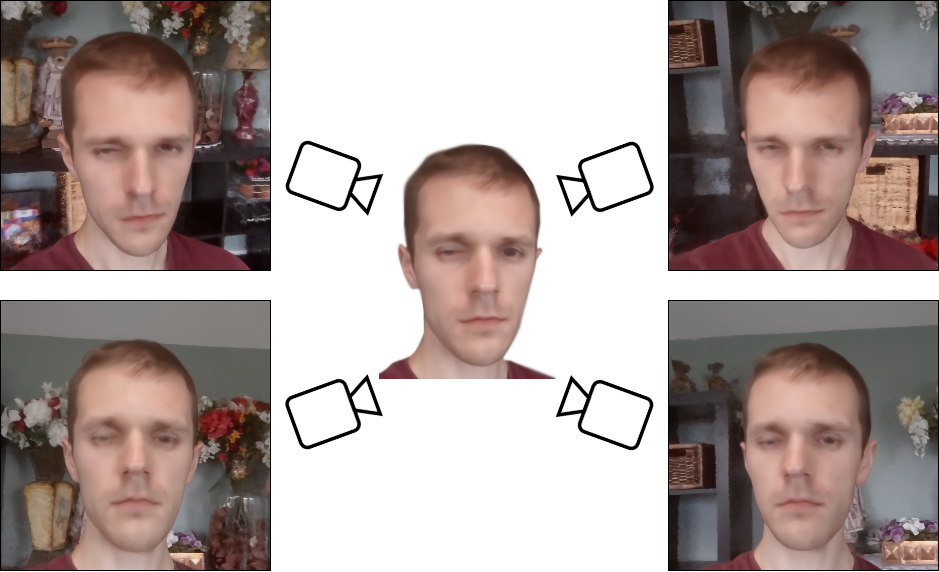
\includegraphics[width=\linewidth]{fig/\conerfdirname/assets/teaser/central.png}
    \subcaption{novel views}
  \end{subfigure}
  \hfill{}
  \begin{subfigure}[b]{0.374\linewidth}
    \centering
    \includegraphics[width=\linewidth]{fig/\conerfdirname/assets/teaser/attributes.pdf}
    \subcaption{novel attributes}
  \end{subfigure}
  \endgroup
}

\fboxsep=0pt % padding thickness
\fboxrule=0.4pt % border thickness
\newcommand{\conerfteaserfigure}{
  \begin{figure}
    \centering
    \teasernobox
    \caption{
      {\bf Teaser --}
      We train a controllable neural radiance field from multiple views of a
      dynamic 3D scene, under varying poses and attributes; in this example
      eye being open/closed and mouth smiling/frowning.
      Given only six annotations (a), our method provides full control over
      the scene appearance, allowing us to synthesize (b) novel views and (c)
      novel attributes, including attribute combinations that were
      \textit{never seen} in the training data~(green box).
    }
    \label{fig:conerf-teaser}
  \end{figure}

}



\conerfteaserfigure
\section{Abstract}
  Decoupling lighting from geometry using unconstrained photo collections is
  notoriously challenging.
  Solving it would benefit many users as creating complex 3D assets takes days
  of manual labor.
  Many previous works have attempted to address this issue, often at the
  expense of output fidelity, which questions the practicality of such
  methods.
  We introduce \lumigauss---a technique that tackles 3D reconstruction of
  scenes and environmental lighting through 2D Gaussian Splatting.
  Our approach yields high-quality scene reconstructions and enables realistic
  lighting synthesis under novel environment maps.
  We also propose a method for enhancing the quality of shadows, common in
  outdoor scenes, by exploiting spherical harmonics properties.
  Our approach facilitates seamless integration with game engines and enables
  the use of fast precomputed radiance transfer.
  We validate our method on the NeRF-OSR dataset, demonstrating superior
  performance over baseline methods.
  Moreover, \lumigauss can synthesize realistic images for unseen environment
  maps.

\chapter{Introduction}
\label{chap:introduction}

                   With the advent of deep learning, research have been
                   exploring varying ways to apply it to computer graphics.
One of the most recent and promising approaches is neural rendering.
Neural rendering is a field that combines deep learning and computer graphics
to generate realistic images of 3D scenes.
The neural radiance field (NeRF) is a popular neural rendering technique that
represents a 3D scene as a continuous function that maps 3D coordinates to
radiance values.
NeRF has shown impressive results in generating photorealistic images of 3D
scenes.
However, NeRF has limitations in terms of memory and computational
requirements, which makes it difficult to scale to large scenes.

                   To alleviate the problem, \textcite{kerbl20233d} proposed a
                   new technique---3D Gaussian Splatting (3DGS).
3DGS is a neural rendering technique that represents a 3D scene as a set of 3D Gaussian that are splatted to an image space using algorithm proposed by~\textcite{zwicker2001ewa}.
 In contrast to NeRF, 3DGS is more memory efficient and can be used to render
 large scenes.
It can also render scenes with millions of points in real-time on a single
GPU.

                   In this thesis, we focus on those two milestone techniques
                   in neural rendering and address their fundamental
                   problem---lack of controllability.

\section{Motivation and challenges}

  NeRF and 3DGS are both impressive techniques that can generate realistic
  images.
  However, a single scene representation needs to be trained on a high-end GPU
  for hours or even days just to render a novel view at the inference time.
  However, any type of controllability is difficult to achieve with those
  models.
  That includes changing the lighting conditions, subject's attributes or even
  the scene itself.
  We see imbuing those models with controllability as a an important step
  towards making them more useful in practice.
  Our proposed models are designed to address this issue.

  One may ask why the controllability is a feat sought after to be researched.
  We see the inspiration in how human artists work.
  Imagine an artist working on 3D game where they need an asset, like a 3D
  mesh, to be created.
  Such a mesh takes much effort since it includes modeling, creating a UV map
  which can then be textured.
  After the process is finish, the artist's supervisor may task him to change
  the model to some extent which requires the artist to redo all the effort
  again.
  Such a process is not limited to 3D assets as meshes and could be applied to
  3DGS or NeRF.
  However, 3DGS and NeRFs are volumetric in nature.
  Our exploited and well-established practices no longer apply to them since
  volumetric representations do not have the underlying surface
  representation.
  For that reason, we see a couple of avenues which we explore in this thesis.

  Firstly, \textcite{park2021nerfies} proposed NeRFies, a model that creates a
  volumetric representation of a person from a self-captured sequence with a
  phone camera.
  Since the inception of NeRFs~\cite{mildenhall2020nerf}, it was among the
  first works the achieved such a high quality of reconstructions from a
  casual videos.
  In its primal form, NeRFies were unable to control the avatar in any other
  way than by a linear interpolation of latent embeddings that embedded the
  video's time dimension.
  The follow-up work, HyperNeRF~\cite{park2021hypernerf} handles this issue by
  projecting the learnable embeddings with $\latentdimension$ onto a
  lower-dimensional space~$\real^\projecteddimension$ where
  $\projecteddimension {\ll}\latentdimension$.
  After the assumption that the $\projecteddimension{=}2$ is enough to explain
  the sequence variability, that projected embedding becomes a 2-dimensional
  space that can be traversed in an interpretable way.
  However, that space is not intuitive since the projection is a non-linear
  operation and one cannot predict how values affect the results.
  To mitigate that issue, we propose to leverage smoothness of Multilayer
  Perceptrons (MLPs)~\cite{tancik2020fourier,park2021nerfies} to constrain the
  projection via sparse supervision.
  We realize our approach as a weakly-supervised MLP that out of many images
  from the sequence (we assume at least 100 frames in our work) only a few are
  provided with a coarse annotation.
  Such annotations denote what values a chosen attribute takes and where its
  effect spans in the image space.
  We show that our method, which we dubbed CoNeRF~\cite{kania2022conerf} and
  published at the CVPR 2022 conference, imbues NeRFs with a flexible
  editability feature without the lose of the rendering quality.

  Secondly, approaches such as CoNeRF~\cite{kania2022conerf},
  EditNeRF~\cite{liu2021editing} or FigNeRF~\cite{xie2021fig} focus solely on
  static elements of the scene, hence their controllability is limited to
  changing colors or textures in general.
  HyperNeRF~\cite{park2021hypernerf} arises as a potential solution due to its
  ability to model object deformations.
  However, our initial experiments showed that those changes cannot handle
  motions that affect a subject globally, \eg, jumping jacks performed by a
  person.
  To solve the issue, \textcite{fang2022fast} proposes to model the
  deformation via a multi-scale voxel structure which works well in the
  synthetic setting, such as the one proposed by~\textcite{pumarola2021d}.

  There exists a plethora of works that approach the problem from the another
  angle---instead of modeling the motion purely from data, they use a template
  model in the form of a 3D mesh to canonicalize deformed
  points~\cite{zielonka2022instant}.
  Such methods rely on the accuracy of the \textit{registration}, \ie, fitting
  the template mesh to subject.
  Since the registration methods~\cite{feng2021learning, zielonka2022towards}
  are imperfect estimators, they inherently contain registration errors.
  Those deviations are exacerbated by learnable radiance field models which
  assume a perfectly calibrated scene.
  The authors of those approaches usually mitigate the issue with additional
  latent space~\cite{grassal2022neural,kania2022conerf,martin2021nerfw} that
  requires thousands of video frames to learn an avatar of high-fidelity that
  reacts correctly to deformations such as wrinkles on the forehead.
  At the same time, performing the registration on the large scale is
  costly~\cite{cao2022authentic}.
  In this thesis, we seek a remedy for those obstacles.
  We propose a method that is data-efficient, easy to improve with a minimal
  user input and can model realistic deformation dependent changes in the
  subject.
  Inspired by classical methods in character texturing~\cite{oat2007animated}
  and motion modeling~\cite{lewis2014practice}, we propose
  BlendFields~\cite{kania2023blendfields}, an \textit{homage} to traditional
  blendshapes~\cite{lewis2014practice}.
  We build on VolTeMorph's~\cite{garbin2024voltemorph} approach to point
  canonicalization to provide a data-efficient way to control the character.
  We further introduce a physically-based mixture of predefined, learned from
  data wrinkle templates that represent expression-dependent skin
  deformations.
  Our proposed was acknowledged by the reviewers and was accepted to the CVPR
  2023 conference.

  Thirdly, having the texture and coarse mesh-based controllability, we strive
  for control scene settings directly.
  The inverse rendering of 3D scenes is an ill-posed problem where many
  different lighting settings may explain the same light
  effects~\cite{patow2003survey}.
  To facilitate solving the problem, many approaches use datasets of single
  object's images captured under different lighting
  conditions~\cite{chen2022hallucinated,yang2023crnerf,rudnev2022nerfosr}.
  These approaches cannot decouple albedo from the lighting
  effects~\cite{chen2022hallucinated,yang2023crnerf} or need additional neural
  networks to predict correct shadows~\cite{rudnev2022nerfosr} which limits
  methods' practicality.
  We propose to use recently proposed 2D Gaussian Splatting~\cite{huang20242d}
  which exhibit remarkable quality of the surface reconstruction.
  Together with our precomputed radiance transfer from classical computer
  graphics approaches~\cite{slomp2006gentle,ramamoorthi2001envmap}, our
  LumiGauss achieves state-of-the-art reconstruction quality with the ability
  to render novel lighting conditions with high fidelity.
  Our work received positive reviews for the WACV 2025 conference.

  Finally, volumetric representation are computationally intensive to render,
  compared to the traditional mesh representation.
  For NeRFs~\cite{mildenhall2020nerf}, it takes seven days on V100 NVidia GPU
  to train for single scene, and more than 60 seconds to render a single
  image---way beyond any practical applications.
  Although many approaches have been proposed to speed up the rendering
  process~\cite{garbin2021fastnerf,yu2021plenoctrees,reiser2021kilonerf,hedman2021baking,mueller2022instant},
  they usually make a trade-off between memory requirements, quality, and
  rendering speed.
  3D Gaussian Splatting~\cite{kerbl20233d} (3DGS) rose as an alternative to NeRF, offering both high-quality rendering at interactive frame rates.
  However, those frame rates could be achieved with the most advanced GPU
  units available at that time.
  As we see the potential in 3DGS to be a viable canonical representation for
  3D data, akin to 3D meshes, a need for its adaptability to different
  computational resources exists.
  Meshes can be adapted easily with levels of detail (LoD) approaches that
  remove detail from meshes that do not affect the general object's perception
  if necessary.

\section{Research objectives}
  In this thesis, we explore different avenues of radiance field
  controllability.
  With this goal in mind, we aim at answering the following research questions:
  \begin{enumerate}[label=(\textbf{RQ \arabic*})]
    \item \label{enum:texturing}
          Can we imbue a Neural Radiance Field (NeRF) with a controllability
          by providing sparse annotations to the training dataset?
          How many annotations suffice to learn smooth interpolation
          capabilities between controlled values?

    \item \label{enum:movement}
          Are extreme facial expressions known from the literature sufficient
          to learn expression-dependent details that extrapolate to
          expressions unseen at the training time?

    \item \label{enum:lighting}
          Is it possible to learn an underlying radiance transfer function of
          a scene from images taken in ``in-the-wild'' setting?
          Can such a transfer function generalize to unknown environment maps?

    \item \label{enum:resources}
          How to learn a single 3D Gaussian Splatting (3DGS) representation
          that can be adapted to different computational regimes at inference
          time in a feed-forward mode?
  \end{enumerate}

  Each of these questions is a representative of possible among many others
  controllability directions for radiance fields.
  In case of this thesis, we present summarize our methods as controls of:
  texture~\cite{kania2022conerf,kania2023blendfields},
  shape~\cite{kania2023blendfields}, lightning~\cite{kaleta2024lumigauss} and
  use of resources~\cite{kania2024clog}.
  To answer~\ref{enum:texturing}, we describe our
  CoNeRF~\cite{kania2022conerf}.
  It is one of the pioneering works that uses sparsely annotated frames to
  continuously control the subject in a post-hoc manner.
  We leverage the fact that MLP used in NeRFs are smooth functions biased
  towards low frequency signals~\cite{tancik2020fourier}.
  For that reason, NeRF can learn to interpolate smoothly the annotation
  signal between frames of high similarity.
  We show that this assumption is sufficient to obtain both novel view
  synthesis and novel attribute synthesis with a single model.

  We further move towards answering~\ref{enum:movement}.
  We introduce BlendFields~\cite{kania2023blendfields}, achieving two primary
  goals: ability to generalize unknown expressions via a predefined face mesh
  template, and a mixture model of training expressions that can produce
  spatially coherent, expression-dependent wrinkles on the face from as few as
  three expressions.
  In our work, we build on VolTeMorph~\cite{garbin2024voltemorph} to achieve
  to former, and focus on the latter contribution.
  Inspired by texture maps in classical computer graphics
  pipelines~\cite{oat2007animated}, we define a set of learnable radiance
  fields, each being overfit to a particular extreme expression from the
  training set.
  We define an extreme expression as one of the possible expressions involving
  the most facial muscles.
  Building on VolTeMorph~\cite{garbin2024voltemorph} allows us to use an
  underlying tetrahedral mesh to compute physical quantities such as the
  volume change of tetrahedra under a given expression.
  We use those quantities to linearly interpolate between the pretrained
  radiance fields.
  We mix the tetrahedra independently which makes rendering novel expressions
  possible.
  For example, BlendFields can render one of the eyebrows raised while
  maintaining the other in a natural position, which is a difficult expression
  to make for majority of people.

  Our LumiGauss~\cite{kaleta2024lumigauss} answers~\ref{enum:lighting}.
  In contrary to common approaches~\cite{rudnev2022nerfosr}, we posit that the
  radiance transfer function known among computer graphics
  researchers~\cite{ramamoorthi2001envmap} can be learned from unconstrained
  photo collection under varying lighting conditions.
  To this end, we use 2DGS~\cite{huang20242d} which gives us a smooth shape
  representation, difficult to achieve when using 3DGS~\cite{kerbl20233d}.
  With the use of contributed priors, we induce learning Gaussian's Spherical
  Harmonics such that they correctly react to changing environment maps.
  Not only our approach is fast to train, but renders realistic scenes and
  object's shadows even under novel lighting conditions.

  All the contributions so far are affected by a specific disadvantage---a
  single model needs to be trained from scratch and it can be deployed only on
  high-end hardware.
  We then ask if we can train a single model that is adaptable at inference
  time to different hardware regimes~\ref{enum:resources}.
  We propose CLoG~\cite{kania2024clog} as a potential remedy.
  Our approach uses the fact that one can constrain the number of Gaussians in
  3DGS~\cite{kerbl20233d} to a specific number, such that it can be formed as
  a 2D grid by simple reshape operation.
  With a specific training coarse-to-fine training protocol we contributed,
  the model learns a representation that converges to a high-quality
  volumetric structure.
  In the second training stage, we leverage the fact that Gaussians's can be
  spatially sorted in such a manner that their descriptors are placed next to
  each other if they are similar.
  That forms a low-frequency image which can be modulated with an
  off-the-shelf continuous upsampling architecture~\cite{vasconcelos2023cuf}.
  The architecture outputs a new grid of the given resolution.
  We show in our work that such an approach achieves remarkable results and
  can output any number of Gaussians at inference time with high quality.

\section{Contributions}
  Building on those questions, we structure this thesis in several chapters
  corresponding to the answers.
  An answer is in a form of a scientific article where we introduce the following:
  \begin{itemize}
    \item A novel approach for controlling trained radiance fields with the use of sparsely annotated images from a casually captured data.
    \item A new model capable of blending trained radiance fields from multi-view frames in an interpretable way and extrapolating to novel human expressions for the trained subject.
    \item The first use of Gaussian Splatting methods that learns a coherent shape representation of a subject and an ability to distill the varying lighting conditions in the data to a radiance transfer function.
    \item A novel paradigm for learning Gaussian Splatting models as 2D grids to achieve flexibility to adapt the model to different computational regimes at inference time.
  \end{itemize}

  % not using primes (not canonicalized parameters)
\begin{figure}
  \centering
  \begin{subfigure}[t]{0.38\linewidth}
    \centering
    \includegraphics[width=\linewidth]{assets/conerf/img/beta-importance-annotations.pdf}
    \caption{annotated samples}
  \end{subfigure}
  \hfill{}
  \begin{subfigure}[t]{0.595\linewidth}
    \centering
    \includegraphics[width=\linewidth]{assets/conerf/img/beta-importance-preds.pdf}
    \caption{renderings from the trained model}
  \end{subfigure}
  \caption{{\bf Example with annotations and controlled attributes --}
    We show an example of how our \conerf is capable of controlling attributes
    selected sparse annotations at the training time.
    Top row shows possible value combinations ($\color{red}{-}$ denoting closed
    eye, $\color{orange}{0}$ neutral position and $\color{green}{+}$ an open eye)
    and $\{\bbeta_1,\bbeta_2\}$ possible values of attributes that are not
    explicitly learned from the annotations but purely from data (please
    see~\cref{chap:conerf} for further explanation).
  }
  \label{fig:conerf-teaser}
\end{figure}
  \subsection{Texture from Partial Information}
    Existing NeRF-based approaches in 2021 were simple models---they were
    overfit to a single subject, for a new subject the model needed to be
    retrained from scratch, and the editability capabilities were
    limited~\cite{liu2021editing}.
    NeRFactor~\cite{zhang2021nerfactor} could be considered a more
    sophisticated model.
    However, it worked only for simple scene with calibrated scenes and could
    not handle any motion.

    We approach those issues in our CoNeRF~\cite{kania2022conerf} published at
    the CVPR 2021 conference.
    Inspired by HyperNeRF~\cite{park2021hypernerf}, we propose to revisit the
    weak supervision in the context of radiance fields.
    Specifically, under an assumption that one can provide a few of sparse
    annotations to the dataset, we can leverage the smoothness of the neural
    networks to propagate the annotation across the dataset.
    The annotations also consist of what regions in the image space it refers
    to and hence we can train a semantic segmentation radiance fields that
    decouples attribute controls.
    We show an example in~\cref{fig:early-conerf-teaser-intro} where the left
    side represents the annotations present in the data and the right one
    possible manipulations at the inference time.
    We note that those annotations are easy to make in a matter of a few
    minutes for a single dataset.
    However, the complexity of the annotations grows with the number of
    attributes to control.

  \subsection{Expression from Few-Shot Learning}
    \conerf~\cite{kania2022conerf} is capable of rendering complex motions
    given sufficient amount of data and provided annotations.
    However, motions as the ones a person performs daily when speaking are
    infeasible in practice.
    We propose a solution to target that issue.
    We introduce \blendfields~\cite{kania2023blendfields} from the CVPR 2023
    proceedings which learns motion-dependent face deformation from data.
    We build on VolTeMorph~\cite{garbin2024voltemorph} which uses existing
    face template models, such as FLAME~\cite{li2017flame}, to learn a single
    canonical representation, akin to the canonicalization module in CoNeRF.
    Internally, \blendfields creates a tetrahedral cage around the face model.
    For each sample along the ray in NeRF, it moves the points to a ``neutral
    position'', chosen once prior to the training procedure.
    Such a procedure comes insufficient to model realistic facial features,
    such as wrinkles.
    We contribute a novel approach to modeling those deformations.
    We compute a deformation gradient of each tetrahedra for a given
    expression which is a physically-based and easy to interpret quantity.
    The value serves us to smoothly transition face regions textures to
    appropriate colors.
    We obtain the colors from NeRFs branches, each overfit to particular
    expression.
    In principle, \blendfields predicts face bases which are conditioned on
    the face expression vector to output the final point color.
    Our framework works well even when only a few ``extreme'' expressions are
    provided such as grinning face with closed eyes and wide open mouth with
    open eyes.

  \subsection{Light from Unconstrained Images}
    In both approaches above, we tackle the problem of texture
    controllability.
    They assume an ideal case scenario where a capture can be taken in an
    idealized environment with constant camera exposure and lighting.
    Moreover, the produced colors are blended together, making the change of
    light impossible in practice.
    We then ask the questions if we can decouple an intrinsic color of the
    subject and change of that color stemming from the environment light.
    We answer that question with our \lumigauss~\cite{kaleta2024lumigauss}
    published at the WACV 2025 conference that, indeed, we can achieve that by
    learning the radiance transfer function directly from data.
    For that end, we train a 2DGS~\cite{huang20242d} model to obtain a smooth
    and spatially coherent surface of objects.
    On top of the other attributes known from 3DGS~\cite{kerbl20233d}, we
    imbue our Gaussians with additional features corresponding to the radiance
    transfer, expressed as Spherical Harmonics~\cite{green2003grittydetail}.
    We show in our experiments that such a formulation is sufficient to train
    a model that reacts to changing environment maps in a realistic manner and
    renders images of higher fidelity than prior approaches.

  \subsection{Levels of Detail in One Model}
    All the contributions above require considerable computation hardware to
    be trained on and then run inference in near real-time frame rates.
    Drawing an inspiration from the gaming industry where Levels of Details
    (LoD) for meshes is used heavily, we introduce \clog~\cite{kania2024clog}.
    Our approach trains a single Gaussian Splatting model such that it can be
    modulated at inference time and adapted to the target computational
    requirements with a minimal loss on the rendering quality.
    That allows us to democratize the use of 3DGS and deploy a single model
    even on handheld devices.
    We show later that even under a strict case where only 2,000
    Gaussians\footnote{Common 3DGS models can achieve from $10^5$ to even
    $10^6$ Gaussians.
    } can be used, the object is still recognizable.
    The most important contribution of our model is that it is continuous by
    design while the existing baselines assume prior the training the model
    how many LoD the model should comprise at inference.
    To change the size of particular LoD in those baselines requires training
    the whole model from scratch, imposing a significant computational burden.

\section{Thesis outline}
  This thesis is structured as follows.
  We start by introducing the preliminaries related to the Neural Radiance
  Fields and Gaussian Splatting in~\cref{chap:background}---a common theme in
  all works that appear later.
  We then move towards describing CoNeRF~\cite{kania2022conerf}
  in~\cref{chap:conerf}, our approach to control trained neural radiance
  fields by using sparse annotations.
  In~\cref{chap:blendfields}, we describe
  BlendFields~\cite{kania2023blendfields} that can produce realistic
  expression-dependent texture from just a few multi-view frames of the
  subjects.
  \cref{chap:lumigauss} introduces the LumiGauss~\cite{kaleta2024lumigauss}, a Gaussian Splatting model that learns a radiance transfer function for novel lighting rendering capabilities.
  Finally, we bring a general method, CLoG~\cite{kania2024clog}, that uses
  Gaussian Splatting to learn continuous levels of detail while training only
  a single model.
  We conclude the thesis in~\cref{chap:final} where we also explore possible
  future avenues that can be undertaken.

\section{Publications not included in the thesis}
  We attach a list of articles that are related to and can be used to in neural rendering approaches:
  \begin{itemize}
    \item\!\!\!\fullciteallauthors{kania2020ucsg},
    \item\!\!\!\fullciteallauthors{kania2021trajevae},
    \item\!\!\!\!\!\fullciteallauthors{stypulkowski2021representing},
    \item\!\!\!\!\fullciteallauthors{xia2023densify},
    \item\!\!\!\fullciteallauthors{esposito2024geogen},
    \item\!\!\!\!\fullciteallauthors{spurek2024modeling}.
  \end{itemize}


% \clearpage
\section{Related works}
  \label{sec:conerf-related}
  Neural Radiance Fields~\cite{mildenhall2020nerf} provide high-quality
  renderings of scenes from novel views with just a few exemplar images
  captured by a handheld device.
  Various extensions have been suggested to date.
  These include ones that focus on improving the quality of
  results~\cite{martin2021nerf, park2020deformable, park2021hypernerf,
  zhang2020nerf++}, ones that allow a single model to be used for multiple
  scenes~\cite{schwarz2020graf, trevithick2020grf}, and some considering
  controllability of the rendering output at a coarse
  level~\cite{guo2020object, yu2021unsupervised, liu2021editing,
  yang2021learning, xie2021fig, zhang2021nerfactor}, as we detail next.

  In more detail, existing works enable only compositional control of object
  location~\cite{yang2021learning,yu2021unsupervised}, and recent extensions
  also allow for finer-grain reproduction of global illumination
  effects~\cite{guo2020object}.
  NeRFactor~\cite{zhang2021nerfactor} shows one can model albedos and BRDFs,
  and shadows, which can be used to, \eg, edit material, but the manipulation
  they support is limited to what is modeled through the rendering equation.
  CodeNeRF~\cite{jang2021codenerf} and EditNeRF~\cite{liu2021editing} showed
  that one can edit NeRF models by modifying the shape and appearance
  encoding, but they require a curated dataset of objects viewed under
  different views and colors.
  HyperNeRF~\cite{park2021hypernerf}, on the other hand can adapt to unseen
  changes specific to the scene, but learns an arbitrary attribute (ambient)
  space that cannot be supervised, and, as we show in
  \cref{sec:conerf-results}, cannot be easily related to specific local
  attribute within the scene for controllability.

  \paragraph{Explicit supervision}
    One can also condition NeRF representations~\cite{gafni2021dynamic} with
    face attribute predicted by pre-trained face tracking networks, such as
    Face2Face~\cite{thies2016face2face}.
    Similarly, for human bodies, A-NeRF~\cite{su2021anerf} and
    NARF~\cite{noguchi2021neural} use the SMPL~\cite{loper2015smpl} model to
    generate interpretable pose parameters, and
    Neural~Actor~\cite{liu2021neural} further includes normal and texture maps
    for more detailed rendering.
    While these models result in controllable NeRF, they are limited to
    domain-specific control and the availability of a heavily engineered
    control model.

  \paragraph{Controllable neural implicits}
    Controllability of neural 3D \textit{implicit} representations has also
    been addressed by the research community.
    Many works have limited focus on learning \textit{human} neural implicit
    representations while enabling the control via SMPL
    parameters~\cite{loper2015smpl}, or linear blend skinning
    weights~\cite{zheng2021pamir, he2021arch++, saito2021scanimate,
    mihajlovic2021leap, ma2021scale, deng2020nasa, alldieck2021imghum,
    zins2021data}.
    Some initial attempts at learned disentangled of shape and poses have also
    been made in A-SDF~\cite{mu2021sdf}, allowing behavior control of the
    output geometry~(\eg doors open vs.
    closed) while maintaining the general shape.
    However, the approach is limited to controlling $\text{SE}(3)$
    articulation of objects, and requires dense 3D supervision.
  \subsection{Neural Radiance Field (NeRF)}
    For completeness, we briefly discuss NeRF before diving into the details
    of our method.
    A Neural Radiance Field captures a volumetric representation of a specific
    scene within the weights of a neural network.
    As input, it receives a sample position~$\bx$ and a view direction~$\bv$
    and outputs the density of the scene $\sigma$ at position~$\bx$ as well as
    the color~$\bc$ at position~$\bx$ as seen from view direction~$\bv$.
    One then renders image pixels~$\bC$ via volume
    rendering~\cite{kajiya1984ray}.
    In more detail, $\bx$ is defined by observing rays~$\br(t)$ as
    \mbox{$\bx=\br(t)$}, where $t$ parameterizes at which point of the ray you
    are computing for.
    One then renders the color of each pixel $\bC(\br)$ by computing
    \begin{equation}
      \bC\left(\br\right) = \int_{t_n}^{t_f} T(t) \sigma\left(\br(t)\right) \bc\left(\br(t), \bv\right) dt
      \;,
      \label{eq:conerf-volume_render}
    \end{equation}
    where $\bv$ is the viewing angle of the ray $\br$, $t_n$ and $t_f$ are the near and far planes of the rendering volume, and
    \begin{equation}
      T(t) = \exp \left ( - \int_{t_n}^t \sigma({\bf r}(s)) ds \right ) \;,
      \end{equation} is the accumulated transmittance.
    Integration in \cref{eq:conerf-volume_render} is typically done via
    numerical integration~\cite{mildenhall2020nerf}.

  \subsection{HyperNeRF}
    Note that in its original formulation~\cref{eq:conerf-volume_render} is
    only able to model \textit{static} scenes.
    Various recent works~\cite{park2020deformable, park2021hypernerf,
    tretschk2021non} have been proposed to explicitly account for possible
    appearance changes in a scene (for example, temporal changes in a video).
    To achieve this, they introduce the notion of \textit{canonical} \textit{hyperspace} -- more formally given a 3D query point $\bx$ and the collection $\pars$ of all parameters that describe the model, they define:
    \begin{align}
      \Canonicalizer(\bx)         & \equiv \Canonicalizer(\bx \given \bbeta, \pars ), \quad                 & \text{Canonicalizer} \label{eq:conerf-canonicalizer} \\
      \bbeta(\bx)                 & \equiv \hypermap (\bx \given \bbeta, \pars ), \quad                     & \text{Hyper~Map} \label{eq:conerf-hypermap}          \\
      \bc(\point), \sigma(\point) & = \Representation(\Canonicalizer(\bx), \bbeta(\bx) \given \pars). \quad & \text{Hyper~NeRF}
      \label{eq:conerf-hypernerf}
    \end{align}
    where the location is canonicalized via a canonicalizer $\Canonicalizer$, and the appearances, represented by $\bbeta$, are mapped to a hyperspace via $\hypermap$, which are then utilized by another neural network $\Representation$ to retrieve the color $\bc$ and the density $\sigma$ at the query location.
    Note throughout this paper we denote $\latent$ to indicates a latent code,
    while $\latent(\point)$ to indicate the corresponding field generated by
    the hypermap lifting.
    With this latent lifting, these methods render the scene via
    \cref{eq:conerf-volume_render}.
    Note that the original NeRF model can be thought of the case where
    $\Canonicalizer$ and $\hypermap$ are identity mappings.


% \clearpage
\begin{figure}
  \centering
  \begin{subfigure}[b]{0.39\linewidth}
    \centering
    \includegraphics[width=\linewidth]{fig/\conerfdirname/assets/implicit.pdf}
    \vspace{0.0em}
    \caption{Neural radiance field with lifting~\cite{park2021hypernerf}}
    \label{fig:conerf-implicit}
  \end{subfigure}
  \hfill
  \begin{subfigure}[b]{0.60\linewidth}
    \centering
    \includegraphics[width=\linewidth]{fig/\conerfdirname/assets/lac.pdf}
    \caption{Controllable neural radiance field (our method)}
    \label{fig:conerf-laced-implicit}
  \end{subfigure}
  \vspace{-0.7em}
  \caption{{\bf Framework -- }
    We depict in (a) the HyperNeRF~\cite{park2021hypernerf} formulation, and
    (b) our Controllable-NeRF~(CoNeRF).
    In (a), both point coordinates $\mathbf{x}$ and latent representation
    $\boldsymbol{\beta}$ are respectively processed by a canonicalizer
    $\Canonicalizer$ and a hyper map $\hypermap$, which are then turned into
    radiance and density field values by $\Representation$.
    In (b), we introduce regressors $\Attribute$ and $\MaskNet$ that regress
    the attribute and the corresponding mask that enable few-shot
    attribute-based control of the NeRF model.
    See~\cref{sec:conerf-inference} for details.
  }
  \label{fig:conerf-pipeline}
\end{figure}
\section{Controllable NeRF (CoNeRF)}
  Given a collection of $\nImages$ color images $\images \in [0,1]^{\width \times \height \times 3}$, we train our controllable neural radiance field model by an auto-decoding optimization~\cite{park2019deepsdf} whose losses can be grouped into two main subsets:
  \begin{align}
    \argmin_{\allpars=\pars, \latents}
    \underbrace{\loss{rep}(\allpars \given \images)}_\text{\cref{sec:conerf-autodecode}}{+}
    \underbrace{\loss{ctrl}(\allpars \given
      \{\Mask^\gt_{\iImage, \iAttribute} \}, \{\attribute^\gt_{\iImage,\iAttribute}\} )}_\text{\cref{sec:conerf-control}}
    .
  \end{align}
  The first group consists of the classical HyperNeRF~\cite{park2021hypernerf} auto-decoder losses, attempting to optimize neural network parameters $\pars$ jointly with latent codes $\latents$ to \textit{reproduce} the corresponding input images $\images$:
  \begin{align}
    \loss{rep}(\cdot) =
    \loss{recon}(\pars, \latents \given \images) +
    \loss{enc}(\latents)
    .
    \label{eq:conerf-loss_render}
  \end{align}
  The latter allow us to inject \textit{explicit control} into the representation, and are our core contribution:
  \begin{align}
    \loss{ctrl}(\cdot)
     & = \loss{mask}(\pars, \latents \given \{\Mask^\gt_{\iImage, \iAttribute} \})     & \text{g.t. masks}      \\
     & + \loss{attr}(\pars, \latents \given \{\attribute^\gt_{\iImage,\iAttribute}\}). & \text{g.t. attributes}
    \label{eq:loss_control}
  \end{align}
  As mentioned earlier in \cref{sec:conerf-intro}, we aim for a neural 3D
  appearance model that is controlled by a collection of attributes
  $\attributes {=} \{\attribute_\iAttribute\}$, and we expect each image to be
  a manifestation of a different value of attributes, that is, each image
  $\image_\iImage$, and hence each latent code $\latent_\iImage$, will have a
  corresponding attribute~$\attributes_\iImage$.
  The learnable connection between latent codes $\latent$ and the attributes
  $\attributes$, which we represent via regressors, is detailed
  in~\cref{sec:conerf-inference}.

  \subsection{Reconstruction losses}
    \label{sec:conerf-autodecode}
    The primary loss guiding the training of the NeRF model is the
    reconstruction loss, which simply aims to reconstruct observations
    $\images$.
    As in other neural radiance field models~\cite{mildenhall2020nerf, martin2021nerfw, park2020deformable, park2021hypernerf} we simply minimize the L2 photometric reconstruction error with respect to ground truth images:
    \begin{equation}
      \loss{recon}(\cdot) = \sum_\iImage \expect_{\ray \sim \image_\iImage} \left[ \left\|\bC(\ray \given \latent_\iImage, \pars)-\bC^\text{gt}(\ray) \right\|_2^2 \right]
      .
      \label{eq:conerf-recon}
    \end{equation}
    As is typical in auto-decoders, and following~\cite{park2019deepsdf}, we impose a zero-mean Gaussian prior on the latent codes~$\latents$:
    \begin{equation}
      \loss{enc}(\cdot) = \sum_\iImage \left\| \latent_\iImage \right\|^2_2
      .
      \label{eq:conerf-latent_prior}
    \end{equation}

  \subsection{Control losses}
    \label{sec:conerf-control}
    The user defines a \textit{discrete} set of $\nAttributes$ number of
    attributes that they seek to control, that are \textit{sparsely}
    supervised across frames---we only supervise attributes \textit{when} we
    have an annotation, and let others be discovered on their own throughout
    the training process, as guided by~\cref{eq:conerf-loss_render}.
    More specifically, for a particular image $\image_\iImage$, and a particular attribute $\attribute_\iAttribute$, the user specifies the quantities:
    \begin{itemize}
      \item $\attribute_{\iImage, \iAttribute} \in [-1,1]$: specifying the value for the $\iAttribute$-th attribute in the $\iImage$-th image; see the \textit{sliders} in~\cref{fig:conerf-teaser};
      \item $\Mask_{\iImage, \iAttribute} \in [0,1]^{\width \times \height}$: roughly specifying the image region that is controlled by the $\iAttribute$-th attribute in the $\iImage$-th image; see the \textit{masks} in~\cref{fig:conerf-teaser}.
    \end{itemize}
    To formalize sparse supervision, we employ an indicator function
    $\indicator_{\iImage, \iAttribute}$, where $\indicator_{\iImage,
    \iAttribute}=1$ if an annotation for attribute $\iAttribute$ for image
    $\iImage$ is provided, otherwise $\indicator_{\iImage, \iAttribute}=0$.
    We then write the loss for \textit{attribute} supervision as:
    \begin{equation}
      \loss{attr}(\cdot) =
      \sum_\iImage \sum_\iAttribute
      \indicator_{\iImage, \iAttribute}
      |\attribute_{\iImage,\iAttribute} - \attribute^\gt_{\iImage,\iAttribute}|^2
      .
    \end{equation}

    For the mask few-shot supervision, \
    we employ the volume rendering in~\cref{eq:conerf-volren} to project the 3D volumetric neural mask field $\mask_\iAttribute(\bx)$ into image space, and then supervise it as:
    \newcommand{\crossentropy}[2]{\text{CE}\left(#1,#2\right)}
    \begin{equation}
      \loss{mask}(\cdot) \!= \!\!\sum_{\iImage, \iAttribute}
      \indicator_{\iImage, \iAttribute} \:
      \expect_\ray
      \left[
        \crossentropy
        {\Mask(\ray \given \latent_\iImage, \pars)}
        {\Mask^\gt_{\iImage, \iAttribute}(\ray)}
        \right]
      ,
      \label{eq:conerf-mask}
    \end{equation}
    where $\crossentropy{\cdot}{\cdot}$ denotes cross entropy, and the field $\sigma(\bx)$ in~\cref{eq:conerf-volren} is learned by minimizing~\cref{eq:conerf-recon}.
    Importantly, as we do not wish for~\cref{eq:conerf-mask} to interfere with
    the training of the underlying 3D representation learned through
    \cref{eq:conerf-recon}, we \textit{stop gradients}
    in~\cref{eq:conerf-mask} w.r.t. $\sigma(\bx)$.
    Furthermore, in practice, because the attribute mask vs.
    background distribution can be highly imbalanced depending on which attribute the user is trying to control (\eg an eye only covers a very small portion of an image), we employ a \textit{focal loss}~\cite{lin2017focal} in place of the standard cross entropy loss.

  \subsection{Controlling and rendering images}
    \label{sec:conerf-inference}
    In what follows, we drop the image subscript $\iImage$ to simplify
    notation without any loss of generality.
    Given a $B$-dimensional latent code $\latent$ representing the 3D scene behind an image, we derive a mapping to our $A$ attributes via a neural map $\Attribute$ with learnable parameters $\pars$:
    \begin{equation}
      \{ \attribute_\iAttribute \} = \AttributeNet(\latent \given \pars), \quad
      \AttributeNet : \real^\latentDim \rightarrow [0,1]^\nAttributes
      ,
    \end{equation}
    where these correspond to the \textit{sliders} in~\cref{fig:conerf-teaser}.
    In the same spirit of~\cref{eq:conerf-hypermap}, to allow for complex
    topological changes that may not be represented by the change in a single
    scalar value alone, we lift the attributes to a hyperspace.
    In addition, since each attribute governs different aspects of the scene, we employ \textit{per-attribute} learnable hypermaps $\{\hypermap_\iAttribute\}$, which we write:
    \begin{align}
      \attribute_\iAttribute(\point) & = \hypermap_\iAttribute(\point, \attribute_\iAttribute \given \pars) \quad \hypermap_\iAttribute: \real^3 \times \real \rightarrow \real^\hyperAttributeDim
      .
    \end{align}
    Note that while $\attribute_\iAttribute$ is a scalar \textit{value},
    $\attribute_\iAttribute(\point)$ is a \textit{field} that can be queried
    at any point $\point$ in space.
    These fields are concatenated to form
    $\attributes(\point)=\{\attribute_\iAttribute(\point)\}$.

    We then provide all this information to generate an \textit{attribute
    masking field} via a network $\MaskNet(\cdot \given \pars)$.
    This field determines which attribute \textit{attends} to which position in space~$\point$:
    \begin{align}
      \label{eq:conerf-mask_c}
      \mask_0(\point) & \oplus \mask(\point) = \MaskNet(\Canonicalizer(\point), \bbeta(\point), \attributes(\point) \given \pars),                   \\
      \MaskNet        & : \real^3 \times \real^\latentDim \times \real^{\nAttributes \times \hyperAttributeDim} \rightarrow \real^{\nAttributes+1}_+
      ,
    \end{align}
    where $\oplus$ is a concatenation operator, $\mask(\point){=}\{\mask_\iAttribute(\point)\}$, and the additional mask $\mask_0(\point)$ denotes space that is not affected by \textit{any} attribute.
    Note that because the mask location should be affected by both the
    particular attribute of interest (\eg, the selected eye status) and the
    global appearance of the scene (\eg, head movement), $\MaskNet$ takes both
    $\bbeta(\point)$ and $\attributes(\point)$ as input in addition to
    $\Canonicalizer(\point)$.
    In addition, because the mask is modeling the attention related to attributes, collectively, these masks satisfy the partition of unity property:
    \begin{align}
      \mask_0(\point) + \Sigma_\iAttribute [\mask_\iAttribute(\point)] = 1 \quad \forall \point \in \real^3
      .
    \end{align}
    Finally, in a similar spirit to~\cref{eq:conerf-hypernerf}, all of this information is processed by a neural network that produces the desired radiance and density fields used in volume rendering:
    \begin{equation}
      \begin{rcases}
        \bc(\point) \\
        \sigma(\point)
      \end{rcases} \!\!=\! \Representation(\Canonicalizer(\point),
      \underbrace{\mask(\point) \odot \attributes(\point)}_\text{attribute controls},
      \underbrace{\mask_0(\point) \cdot \latent(\point)}_\text{everything else}
      \given \pars)
      .
      \label{eq:conerf-representation}
    \end{equation}
    In particular, note that $\mask(\point){=}0$ implies
    $\mask_0(\point){=}1$, hence our solution has the capability of reverting
    to classical HyperNeRF~\cref{eq:conerf-hypernerf}, where all change in the
    scene is globally encoded in $\bbeta(\point)$.
    Finally, these fields can be used to render the mask in image space, following a process analogous to volume rendering of radiance:
    \begin{equation}
      \Mask(\ray\given\allpars) \!=\!\!
      \int_{t_n}^{t_f} \!\!\!\!
      T(t) \cdot \sigma(\br(t)) \cdot [\mask_0(\ray(t)) \oplus \mask(\ray(t))]
      \, dt .
      \label{eq:conerf-volren}
    \end{equation}
    We depict our inference flow in~\cref{fig:conerf-pipeline}~(b).

  \subsection{Implementation details}
    We implement our method for NeRF based on the JAX \cite{jax2018github}
    implementation of HyperNeRF~\cite{park2021hypernerf}.
    We use both the scheduled windowed positional encoding and weight
    initialization of \cite{park2020deformable}, as well as the coarse-to-fine
    training strategy~\cite{park2021hypernerf}.

    Besides the newly added networks, we follow the same architecture as
    HyperNeRF.
    For the attribute network $\Attribute$ we use a six-layer multi-layer
    perceptron (MLP) with 32 neurons at each layer, with a skip connection at
    the fifth layer, following \cite{park2020deformable,park2021hypernerf}.
    For the lifting network $\hypermap_\iAttribute$, we use the same
    architecture as $\hypermap$, except for the input and output dimension
    sizes.
    For the masking network $\MaskNet$ we use a four-layer MLP with 128
    neurons at each layer, followed by an additional 64 neuron layer with a
    skip connection.
    The network $\Representation$ also shares the same architecture as
    HyperNeRF, but with a different input dimension size to accommodate for
    the changes our method introduces.

    \paragraph{2D implementation}
      To show that our idea is not limited to neural radiance fields, we also
      test a 2D version of our framework that can be used to directly
      represent images, without going through volume rendering.
      We use the same architecture and training procedure as in the NeRF case,
      with the exception that we do not predict the density $\sigma$, and we
      also do not have the notion of depth---each ray is directly the pixel.
      We center crop each video and resize each frame to be $128\times128$.

    \paragraph{Hyperparameters}
      We train all our NeRF models with $480\times270$ images and with 128
      samples per ray.
      We train for 250k iterations with a batch size of 512 rays.
      During training, we maintain that 10\% of rays are sampled from
      annotated images.
      We set $\loss{attr}=10^{-1}$, $\loss{mask}=10^{-2}$ and
      $\loss{enc}=10^{-4}$.
      For the number of hyper dimensions we set $\hyperAttributeDim = 8$.
      For the 2D implementation experiments, we sample 64 random images from
      the scene and further subsample 1024 pixels from each of them.
      For all experiments we use Adam~\cite{kingma2014adam} with learning rate
      $10^{-4}$ exponentially decaying to $10^{-5}$ in 250k iterations.
      We provide additional details in the supplementary material.
      Training a single model takes around 12 hours on an NVIDIA V100 GPU.

% \clearpage
\begin{figure}
  \centering
  \includegraphics[width=\linewidth]{fig/\conerfdirname/assets/update-attributes.pdf}
  \caption{{\bf Novel view and novel attribute synthesis on real data --}
    We synthesize scenes from a novel view and with a novel attribute
    combination, not seen during training.
    % \ky{
    A naive extension of HyperNeRF, HyperNeRF{+}$\pi$ fails to disentangle
    attributes and results in a modification of the scene irrespectively of
    attribute meaning \eg, opening mouth results in closing eyes at the same
    time.
    % is not what the attributes are describing--- and vice versa. 
    Ours-$\MaskNet$ improves the results, but does not disentangles the
    attribute space, as successfully done by our complete method.
    % results in entanglement.
    The differences between these methods can even lead to complete failure
    cases, as shown in the metronome and the toy car case.
  }
  % \cite{park2021hypernerf} with a projection network $\mathcal{A}$ to predict
  % attribute values $\{\attribute_\iAttribute\}$ causes that changes in the
  % output become entangled, \eg, opening the mouth also closes the
  % eyes.%causes closing eyes. }
  \label{fig:conerf-novel_view}
\end{figure}

\section{Results}
  \label{sec:conerf-results}

  \subsection{Datasets and baselines}

    We evaluate our method on two datasets: real video sequences captured with
    a smartphone ({\it real dataset}) and synthetically rendered sequences
    ({\it synthetic dataset}).
    Here we introduce those datasets and the baselines for our approach.

    \paragraph{Real dataset}
      % We evaluate our method on two types of data: real video sequences
      % captured with a smartphone and synthetically rendered sequences.
      Each of the seven real sequences is 1 minute long and was captured
      either with a Google Pixel 3a or an Apple iPhone 13 Pro.
      Four of them consists of people performing different facial expressions
      including smiling, frowning, closing or opening eyes, and opening mouth.
      % One of the four, we capture only the frontal view of the person, which
      % we reserve for the 2D image experiment.
      For the other three, we captured a toy car changing its shape ({\it
      a.k.a.
        }
      Transformer), a single metronome, and two metronomes beating with
      different rates.
      For one of the four videos depicting people, to use it for the 2D
      implementation case, we captured it with a static camera that shows a
      frontal view of the person.
      All other sequences feature camera motions showing front and sides of
      the object in the center of the scene.
      % \mk{One of the four videos depicting people is captured with a static
      % camera that shows a frontal view of the person, this video is reserved
      % for evaluating the 2D implementation of our method described in the
      % preceding section. All the remaining captures feature a moving camera
      % that captures the front and sides of the objects in the center of the
      % scene.}
      For videos with human subjects, the subjects signed a participant
      consent form, which was approved by a research ethics board.
      We informed the participants that their data will be altered with our
      method.

      We extract frames at 15 FPS which gives approximately 900 frames per
      capture.
      % \KY{do you mean every other frame is validation?}
      Because novel attribute synthesis via user control on real scenes does
      not have a ground truth view---we aim to create scenes with unseen
      attribute combinations---the benefit of our method is best seen
      qualitatively.
      Nonetheless, to quantitatively evaluate the rendering quality, we
      interpolate between two frames and evaluate its quality.
      In more detail, to minimize the chance of the dynamic nature of the
      scene interfering with this assessment, we use every other frame as a
      test frame for the interpolation task.

      % Annotations 
      For all human videos, we define three attributes---one for the status of
      each of the two eyes, and one for the mouth.
      We annotate only six frames per video in this case, specifically the
      frames that contain the extremes of each attribute (\eg, left eye fully
      open).
      For the toy car, we set the shape of the toy car to be an attribute, and
      annotate two extremes from two different view points---when the toy is
      in robot-mode and when it is in car-mode from its left and right side.
      For the metronomes, we consider the state of the pendulum to be the
      attribute and annotate the two frames with the two extremes for the
      single metronome case, and seven frames for the two metronome case as
      the pendulums of the two metronomes are often close to each other and
      required special annotations for these close-up cases;
      see~\cref{fig:conerf-novel_view}.

    \paragraph{Synthetic dataset}
      Since the lack of ground-truth data renders measuring the quality of
      novel attribute synthesis infeasible in practice, we leverage Kubric
      software~\cite{kubric2021github} to generate synthetic dataset, where we
      know exactly the state of each object in the scene.
      % is it is difficult to quantitatively measure novel attribute synthesis
      % with real data, we further use
      We create a simple scene where three 3D objects, the teapot
      \cite{teapot}, the Stanford bunny \cite{bunny}, and Suzanne
      \cite{suzanne}, are placed within the scene and are rendered with
      varying surface colors, which are our attributes;
      see~\cref{fig:conerf-kubric3d}.
      % We create one dataset that is in 3D for the NeRF experiments, and one
      % in 2D, using a top-view camera for the 2D tests. \KY{Below might
      % change---we might just to color changes ;)} \todo{% We move each object
      % in the scene independently of others on a predefined trajectory. }%
      We generate 900 frames for training and 900 frames for testing.
      To ensure that the attribute combination during training is not seen in
      the test scene, we set the attributes to be synchronized for the
      training split, and desynchronized for the test split.
      % \ky{
      We further render the test split from different camera positions than
      the training split to account for novel views.
      % }
      We randomly sample 5\% of the frames with a given attribute for each
      object to be set as the ground-truth attribute.
      During validation, we use attribute values directly to predict the
      image.

    \paragraph{Baselines}
      To evaluate the reconstruction quality of our method, CoNeRF, we compare
      it with four different baselines: \CIRCLE{1}~standard
      NeRF~\cite{mildenhall2020nerf}; \CIRCLE{2}~NeRF+Latent, a simple
      extension to NeRF where we concatenate each coordinate $\bx$ with a
      learnable latent code $\bbeta$ to support appearance changes of the
      scene; \CIRCLE{3}~Nerfies \cite{park2020deformable}; and
      \CIRCLE{4}~HyperNeRF\footnote{We use the version with dynamic plane
      slicing as it consistently outperforms the axis-aligned strategy; see
      \cite{park2021hypernerf} for more details.
      }~\cite{park2021hypernerf}.
      % \ky{
      Additionally, as existing methods do not support attribute-based control
      with a few-shot supervision, we create another baseline \CIRCLE{5} by
      extending HyperNeRF with a simple linear regressor $\pi$ that regresses
      $\bbeta_c$ given $\balpha_c$.
      We call this baseline HyperNeRF{+}$\pi$.
      % } \ky{ We also compare our approach against a %setting with disabled
      % mask part of our %pipeline. } slightly re-written
      To further show the importance of masking, we also compare our approach
      against a stripped-down version of our method, Ours{-}$\MaskNet $, where
      we disable the part of our pipeline responsible for masking.
      All baselines that utilize annotations were trained with the same sparse
      labels as our method.
      % \MK{is the above sentence I added true?} Ours{-}$\MaskNet$ to show its
      % importance.\tom{this sounds like some weird ablation study description}
      % \ky{} where we use $\mathcal{A}$ and $\mathcal{G}$ modules instead of
      % $\mathcal{H}$ (see \cref{fig:laced-implicit}). In short, we project
      % $\bbeta$ with an MLP, supervise the obtained representation with
      % annotations and use it as the latent representation that is processed
      % as in HyperNeRF \cite{park2021hypernerf}. We refer to this baseline as
      % HyperNeRF{+}Proj.

  \subsection{Comparison with the baselines}
    \begin{figure}
  \centering
  \begin{subfigure}[b]{0.164\linewidth}
    \centering
    
\includegraphics[width=\linewidth]{fig/\conerfdirname/assets/annotate/input.png}
    \caption{annotation}
  \end{subfigure}
  \hfill{}
  \begin{subfigure}[b]{0.816\linewidth}
    \centering
    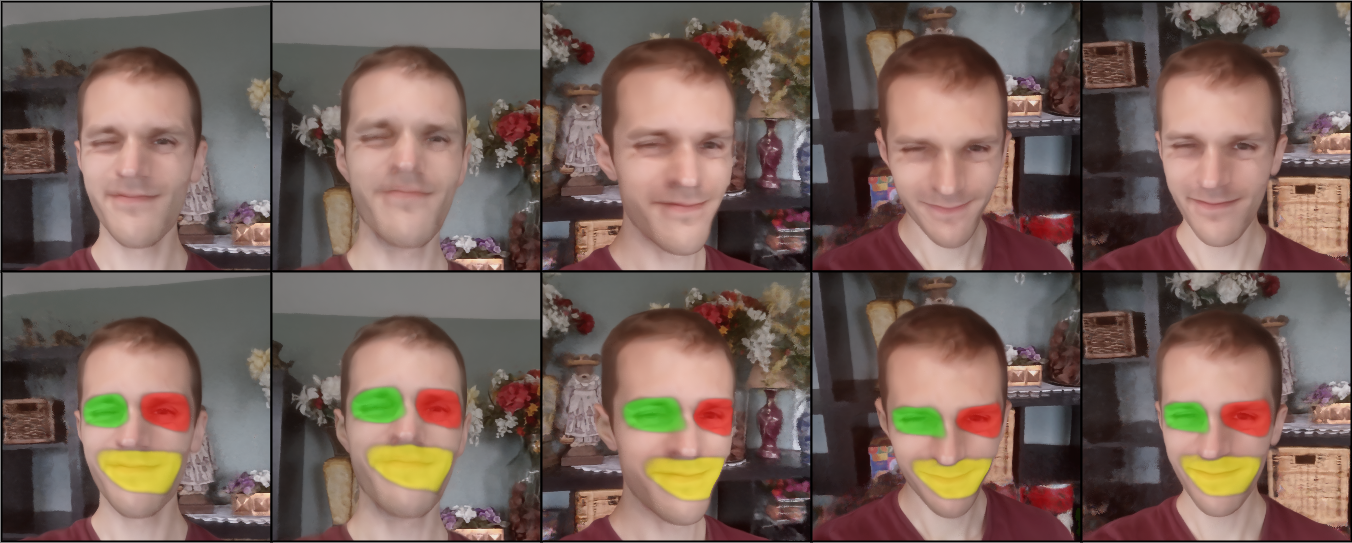
\includegraphics[width=\linewidth]{fig/\conerfdirname/assets/annotate/novel-views.png}
    \caption{unannotated views}
  \end{subfigure}
  \caption{{\bf Annotation example -- }
    We provide only a rough annotation for each attribute, which is enough for
    the method to discover the mask for each attribute across all views
    automatically.
    Bottom row shows masks overlaid on the image.
  }
  \label{fig:conerf-annotate}
\end{figure}

    \paragraph{Qualitative highlights}
      % \ky{%
      We first show qualitative examples of novel attribute and view synthesis
      on the real dataset in \cref{fig:conerf-novel_view}.
      Our method allows for controlling the selected attribute without
      changing other aspects of the image---our control is disentangled.
      This disentanglement allows our method to generate images with attribute
      combinations that were not seen at training time.
      % Our method allows to independently control multiple attributes without
      % the risk of entangling them with each other. In the case of
      % HyperNeRF{+}$\pi$, a simple regression strategy is unable to
      % disentangle the motions that happen within the scene which results in
      % uncontrollable rendering ({\it e.g.,} opening mouth triggered by
      % closing the eyes). 
      On the contrary, as there is no incentive for the learned embeddings of
      HyperNeRF to be disentangled, the simple regression strategy of
      HyperNeRF{+}$\pi$ results in entangled control, where when one tries to
      close/open the mouth it ends up affecting the eyes.
      % \KY{This might need rewrite after Fig3 is finalized}.
      The same phenomenon happens also for Ours{-}$\MaskNet$.
      % is unable to produce a distentangled representation as evidenced by
      % issues like the mouth opening when only the attribute responsible for
      % one of the eyes is modified.
      Moreover, due to the complexity of motions in the scene,
      HyperNeRF{+}$\pi$ fails completely to render novel views of the toy car,
      whereas our method, with only four annotated frames, successfully
      provides both controllability and high-quality renderings.
      % }%
      Please also see \SupplementaryMaterial for more qualitative results,
      including a video demonstration.

      Note that in all of these sequences, we provide highly sparse
      annotations and yet our method learns how each attribute should
      influence the appearance of the scene.
      In \cref{fig:conerf-annotate}, we show an example annotation and how the
      method finds the mask for unannotated views.

      \begin{figure}
  \centering
  \includegraphics[width=0.8\linewidth]{fig/\conerfdirname/assets/kubric3d/synthetic.pdf}
  \caption{{\bf Novel view and novel attribute synthesis on synthetic data -- }
    We show examples of novel view and novel attribute synthesis on synthetic
    data.
    The scene is composed of three objects, where the color of each object is
    their attribute.
    Our method provides control over the color of each object independently,
    whereas both HyperNeRF{+}$\pi$ and Ours{-}$\MaskNet$ fail to deliver
    controllability and results in all three objects having the same attribute
    in the rendered scene.
  }
  \label{fig:conerf-kubric3d}
\end{figure}
      \begin{figure}
  \centering
  \includegraphics[width=0.8\linewidth]{fig/\conerfdirname/assets/kubric3d/synthetic.pdf}
  \caption{{\bf Novel view and novel attribute synthesis on synthetic data -- }
    We show examples of novel view and novel attribute synthesis on synthetic
    data.
    The scene is composed of three objects, where the color of each object is
    their attribute.
    Our method provides control over the color of each object independently,
    whereas both HyperNeRF{+}$\pi$ and Ours{-}$\MaskNet$ fail to deliver
    controllability and results in all three objects having the same attribute
    in the rendered scene.
  }
  \label{fig:conerf-kubric3d}
\end{figure}
    \paragraph{Quantitative results on synthetic dataset}
      To complete the qualitative evaluation of our method, we provide results
      using synthetic dataset with available ground truth.
      We measure Peak Signal-to-Noise Ratio (PSNR), Multi-scale Structural
      Similarity (MS-SSIM)~\cite{wang2003multiscale}, and Learned Perceptual
      Image Patch Similarity (LPIPS)~\cite{zhang2018unreasonable} and report
      them in~\cref{tab:conerf-kubric3d}.
      With only 5\% of the annotations, our method provides the best
      novel-view and novel-attribute synthesis results, as reconfirmed by the
      qualitative examples in~\cref{tab:conerf-kubric3d}.
      As shown, neither HyperNeRF{+}$\pi$ nor Ours{-}$\MaskNet$ is able to
      provide good results in this case, as without disentangled control of
      each attribute, the novel attribute and view settings of each test frame
      cannot be synthesized properly.

    \paragraph{Interpolation task}
      To further verify that our rendering quality does not degrade with the
      introduction of controllability, we evaluate our method on a frame
      interpolation task without any attribute control.
      Unsurprisingly, as shown in~\cref{tab:conerf-sota}, all methods that
      support dynamic scenes work similarly, including ours for interpolation.
      Note that for the interpolation task, we interpolate every other frame,
      in order to minimize the chance of attributes affecting the evaluation.
      Here, we are purely interested in the rendering quality from a novel
      view.

      \begin{table}
  \centering
  \begin{tabular}{@{}lccc@{}}
    \toprule
    Method                     & PSNR $\uparrow$ & MS-SSIM $\uparrow$ & LPIPS $\downarrow$ \\
    \midrule
    NeRF                       & 28.795          & 0.951              & 0.210              \\
    NeRF + Latent              & 32.653          & 0.981              & 0.182              \\
    NeRFies                    & 32.274          & 0.981              & 0.180              \\
    HyperNeRF                  & 32.520          & 0.981              & 0.169              \\
    \midrule
    \textbf{Ours}{-}$\MaskNet$ & 32.061          & 0.979              & 0.167              \\
    \textbf{Ours}              & 32.342          & 0.981              & 0.168              \\

    \bottomrule
  \end{tabular}
  \caption{
    \textbf{Quantitative results (interpolation) -- }
    We report results in terms of PSNR, MS-SSIM, and LPIPS for the
    interpolation task.
    These results are obtained for interpolated view synthesis only, not for
    novel attribute rendering.
    Our method provides similar performance in terms of rendering quality, but
    with controllability.
  } % \caption
  \label{tab:conerf-sota}
\end{table}

      \begin{figure}
  \centering
  \includegraphics[width=0.8\linewidth, trim=0 320 0 0, clip]{fig/\conerfdirname/assets/face.pdf}
  \caption{
    {\bf 2D image generation example -- }
    Our framework also generalizes to direct generation of 2D images.
    Here we show novel attribute synthesis for a webcam video of a person
    making expressions.
    Each individual part of the scene is correctly controlled according to the
    attribute values.
  }
  % }
  \label{fig:conerf-2d-interpolation}
\end{figure}
  \subsection{Direct 2D rendering}
    To verify how our approach generalizes beyond NeRF models and volume
    rendering, we apply our method to videos taken from a single view point,
    creating a 2D rendering task.
    We show in~\cref{fig:conerf-2d-interpolation} a proof-of-concept for
    employing our approach outside of NeRF applications to allow controllable
    neural generative models.

  \subsection{Ablation study}
    \begin{table}
  \centering
  \normalsize
  \setlength{\tabcolsep}{2pt}
  \begin{tabular}{@{}lccc ccc@{}}
    \toprule
          & \multicolumn{3}{c}{Real (interpolation)} & \multicolumn{3}{c}{Synthetic (novel view \& attr.)}                                                                                  \\
    \cmidrule(lr){2-4}
    \cmidrule(lr){5-7}
    Model & PSNR $\uparrow$ & MS-SSIM $\uparrow$ & LPIPS $\downarrow$ & PSNR
    $\uparrow$ & MS-SSIM $\uparrow$ & LPIPS $\downarrow$ \\ \midrule Base
    ($\loss{recon}$) & 32.457 & 0.981 & 0.168 & 24.407 & 0.718 & 0.173 \\
    $+\loss{enc}$ & 32.478 & 0.982 & 0.167 & 27.018 & 0.871 & 0.164 \\ $+
    \loss{enc} +\loss{attr}$ & 32.254 & 0.981 & 0.167 & 27.322 & 0.873 & 0.147
    \\ $+ \loss{enc} + \loss{attr} +\loss{mask}$ & 32.342 & 0.981 & 0.168 &
    \textbf{32.394} & \textbf{0.972} & \textbf{0.139}\\
    \bottomrule\end{tabular} \caption{ \textbf{{Effect of loss functions --}}
    We report the rendering quality of our method as we procedurally introduce
    the loss terms.
    % < \resizebox 
    For controlled rendering with novel views and attributes (synthetic data),
    each loss term adds to the rendering quality, with the $\loss{mask}$ being
    critical.
    For the novel view rendering on real data, addition of loss functions for
    controllability do not have a significant effect on the rendering
    quality---they do no harm.
  } % \caption
  \label{tab:conerf-ablations}
\end{table}
    \paragraph{Loss functions}
      In~\cref{tab:conerf-ablations}, we show how each loss term affects the
      network's performance, contributing to performance improvements.
      When rendering novel views with novel attributes, the full formulation
      is a must, as without all loss terms the performance drops
      significantly---for example, results without $\loss{mask}$ is similar to
      Ours-$\MaskNet$ results in~\cref{tab:conerf-kubric3d} and
      \cref{fig:conerf-kubric3d}.
      In the case of the interpolation task, the additional loss functions for
      controllability have no significant effect on the rendering quality.
      In other words, our controllability losses \textbf{do not interfere}
      with the rendering quality, other than imbuing the framework with
      controllability.
      \vspace{-0.2em}

      \begin{figure}
  \centering
  \includegraphics[width=\linewidth]{fig/\conerfdirname/assets/annotations-differences.pdf}
  \caption{{\bf Effect of annotation quality -- }
    Our method is moderately robust to the quality of annotations.
    We visualize the results for two expressions: frowning and smiling, while
    keeping both eyes in a neutral position.
    Even with wildly varying annotations as shown, the reconstructions are
    reasonably controlled, with the exception of the top row, where we show a
    case where the annotations is too restrictive, resulting in the annotation
    being ignored for one eye.
    We show in bottom row also an interesting case, where the mask is large
    enough to start capturing the correlation among mouth expressions and the
    eye.
  }
  \label{fig:conerf-ablation_annotate}
\end{figure}
    \paragraph{Quality of few shot supervision}
      We test how sensitive our method is against the quality of annotation
      supervision.
      In~\cref{fig:conerf-ablation_annotate} we demonstrate how each
      annotation leads to the final rendering quality.
      Our framework is robust to a moderate degree to the inaccuracies in the
      annotations.
      However, when they are too restrictive, the mask may collapse, as shown
      on the top row.
      Too large of a mask could also lead to moderate entanglement of
      attributes, as shown in the bottom row.
      Still, in all cases, our method provides a reasonable control over what
      is annotated.

      % not using primes (not canonicalized parameters)
\begin{figure}
  \centering
  \begin{subfigure}[t]{0.38\linewidth}
    \centering
    \includegraphics[width=\linewidth]{fig/\conerfdirname/assets/beta-importance-annotations.pdf}
    \caption{annotated samples}
  \end{subfigure}
  \hfill{}
  \begin{subfigure}[t]{0.595\linewidth}
    \centering
    \includegraphics[width=\linewidth]{fig/\conerfdirname/assets/beta-importance-preds.pdf}
    \caption{renderings}
  \end{subfigure}
  \caption{{\bf Example with unannotated attributes --}
    We show an example of how our method performs when a part of the image
    changes appearance, but is not annotated.
    With the annotations in (a), we synthesize the scene with novel view and
    attributes in (b), where the two rows are with different $\bbeta$
    configurations.
    We denote the attribute configuration on the top of each column in (b).
    As shown, the change that is not annotated is simply encoded in the
    per-image encoding $\bbeta$.
  }
  \label{fig:conerf-ablation_unannotated}
\end{figure}
    \paragraph{Unannotated attributes}
      A natural question to ask is then what happens with the unannotated
      changes that may exist in the scene.
      In~\cref{fig:conerf-ablation_unannotated} we show how the method
      performs when annotating only parts of the appearance change within the
      scene.
      The unannotated changes of the scene get encoded as $\bbeta$, as in the
      case of HyperNeRF~\cite{park2021hypernerf}.

% \clearpage
\section{Conclusions}
  \label{sec:lumigauss-conclusions}

  We present \lumigauss---the method capable of decoupling environment
  lighting and albedo of objects from images \textit{in-the-wild}.
  To this end, we apply 2DGS~\cite{huang20242d} to reconstruct the object's
  surface accurately and then use our proposed training components that
  correctly disentangle light properties from the rendered colors.
  As we show in the experiments, our approach achieves better reconstruction
  results than the baselines.
  We also present that one of our contributions---modeling shadows via
  leveraging Spherical Harmonics properties---provides shadows of high
  fidelity that react appropriately to changing environment light.
  \lumigauss is a novel approach in the direction of inverting the rendering process from images \textit{in-the-wild}, reconstructing high-quality scene properties without sacrificing the fidelity of the output.
\section{Acknowledgements}
  \label{sec:conerf-ack}
  We thank Thabo Beeler, JP Lewis, and Mark J.
  Matthews for their fruitful discussions, and Daniel Rebain for helping with
  processing the synthetic dataset.
  The work was partly supported by National Sciences and Engineering Research
  Council of Canada (NSERC), Compute Canada, and Microsoft Mixed Reality \& AI
  Lab.
  This research was funded by Foundation for Polish Science (grant no
  POIR.04.04.00-00-14DE/18-00 carried out within the Team-Net program
  co-financed by the European Union under the European Regional Development
  Fund), National Science Centre, Poland (grant no 2020/39/B/ST6/01511), and
  by Microsoft Research through EMEA PhD Scholarship Programme.
  The authors have applied a CC BY license to any Author Accepted Manuscript
  (AAM) version arising from this submission, in accordance with the grants’
  open access conditions.


% --- repeat the title (AT: haven't found a more elegant way to do this...)
{
\vspace{2.0em}
\centering
\Large
\textbf{CoNeRF: Controllable Neural Radiance Fields} \\
\vspace{0.5em}
 Supplementary Material \\ \vspace{1.0em} }

 \section{Potential social impact} Our motivation for this work was to enable
 the creation of 3D avatars that could be used as communication devices in the
 remote working era.
  As our approach stems from blendshapes~\cite{lewis2014practice}, these
  avatars are easily adjustable via texture coloring and may be used for
  entertainment.
  We note, however, that the potential misuse of our work includes using it as
  deep fakes.
  We highly discourage such usage.
  One of our future directions includes detecting fake images generated by our
  method.
  At the same time, we highlight the importance of \blendfields---in the
  presence of closed technologies~\cite{ma2021pixel,cao2022authentic}, it is
  crucial to democratize techniques for personalized avatar creation.
  We achieve that by limiting the required data volume to train a single
  model.
  As history shows, when given an open, readily available technology for
  generative modeling of images~\cite{rombach2022high}, users can scrutinize
  it with unprecedented thoroughness, thus raising the general awareness of
  potential misuses.

\section{Concurrent Works}
  Gao~\etal~\cite{gao2022reconstructing} and Xu~\etal~\cite{xu2022manvatar}
  also use an interpolation between known expressions to combine multiple
  neural radiance fields trained for those expressions.
  However, their approach interpolates between grids of latent
  vectors~\cite{mueller2022instant} globally.
  The interpolation weights are taken from blendshape coefficients.

  Zielonka~\etal~\cite{zielonka2022instant} use a parametric head model to
  canonicalize 3D points similarly to our ends.
  However, instead of building a tetrahedral cage around the head, they
  smoothly assign each face triangle to 3D points.
  Then they canonicalize points using transformations that each of the
  assigned triangles undergoes for a given expression.
  They concatenate 3D points with the expression code from
  FLAME~\cite{li2017flame} to model expression-dependent effects.

  \begin{table}[!t]
  \centering
  \resizebox{\linewidth}{!}{
    \begin{tabular}{ccccccc}
      \toprule
      \multirow{2}[2]{*}{\# expr.} & \multicolumn{3}{c}{Casual Expressions} & \multicolumn{3}{c}{Novel Pose Synthesis}                                                                                                                                                  \\
      \cmidrule{2-7}
                                   & PSNR $\uparrow$                        & SSIM $\uparrow$                          & LPIPS $\downarrow$                & PSNR $\uparrow$                    & SSIM $\uparrow$                   & LPIPS $\downarrow$                \\
      \midrule
      $\nExpr{=}1$                 & 27.5834                                & 0.9028                                   & 0.0834                            & 28.7589                            & 0.9147                            & 0.0806                            \\
      $\nExpr{=}2$                 & 27.6783                                & 0.9026                                   & 0.0856                            & 29.2859                            & 0.9186                            & 0.0803                            \\
      $\nExpr{=}3$                 & 27.9137                                & 0.9054                                   & 0.0819                            & 29.8551                            & 0.9279                            & 0.0728                            \\
      $\nExpr{=}4$                 & 27.8140                                & 0.9055                                   & 0.0815                            & \cellcolor{secondbestcolor}30.1543 & \cellcolor{secondbestcolor}0.9336 & \cellcolor{secondbestcolor}0.0701 \\
      $\nExpr{=}5$                 & 28.0254                                & 0.9110                                   & \cellcolor{firstbestcolor}0.0778  & \cellcolor{firstbestcolor}30.4721  & \cellcolor{firstbestcolor}0.9372  & \cellcolor{firstbestcolor}0.0688  \\
      \midrule
      $\nExpr{=}6$                 & 28.0517                                & 0.9091                                   & \cellcolor{secondbestcolor}0.0813 & --                                 & --                                & --                                \\
      $\nExpr{=}7$                 & \cellcolor{secondbestcolor}28.2004     & \cellcolor{secondbestcolor}0.9115        & 0.0823                            & --                                 & --                                & --                                \\
      $\nExpr{=}8$                 & \cellcolor{firstbestcolor}28.2542      & \cellcolor{firstbestcolor}0.9124         & 0.0830                            & --                                 & --                                & --                                \\
      \bottomrule
    \end{tabular}
  }
  \caption{\textbf{Number of training expressions} -- {
      We ablate over the number of training expressions.
      We evaluate the model on the captures from the Multiface
      dataset~\cite{wuu2022multiface}.
      We run the model for each possible expression combination for a given
      $\nExpr$ and average the results.
      The best results are colored in \mycoloredbox{firstbestcolor} and the
      second best in \mycoloredbox{secondbestcolor}.
      Increasing the number of available training expressions consistently
      improves the results.
      However, using $\nExpr{=}5$ expressions saturates the quality and using
      $\nExpr{>}5$ brings diminishing improvements.
      We do not report ``Novel Pose Synthesis'' for $\nExpr{>}5$ as we use
      validation expressions and poses to train those models (refer
      to~\cref{subsec:blendfields-realistic-human-captures} for more details).
      % As $\nExpr{=}5$ already consists of extreme expressions, increasing its
      % number further does not improve the results consistently. 
    }
  }
  \label{tab:blendfields-ablation-num-expressions-fix}

\end{table}

\section{Additional results}
  \subsection{Ablating number of expressions}
    We ablate over the number of used expressions during the training.
    To evaluate the effect of the number of expressions, we add consecutive
    frames to the training set (starting from a single, neutral one), \ie, the
    training set has $\iExpr{<}\nExpr$ expressions.
    We train \blendfields for such a set for each subject separately.
    We then average the results for a given $\iExpr$ across subjects.
    We present the results in~\cref{tab:ablation-num-expressions-fix}.
    When selecting the training expressions, we aim to choose those that show
    all wrinkles when combined.
    We can see from~\cref{fig:blendfields-qualitative-ablation-expressions}
    that if removed, \eg, the expressions with eyebrows raised, then the model
    cannot render wrinkles on the forehead.
    In summary, increasing the number of expressions improves the quality
    results with diminishing returns when $\nExpr{>}5$, while $\nExpr{=}5$
    provides a sufficient trade-off between the data capture cost and the
    quality.
    % Moreover, we posit that $\nExpr{=}5$ is enough to capture most facial
    % details and get consistent, high-quality results.

    \begin{figure}[t]
  % \vspace{-2em}
  \centering
  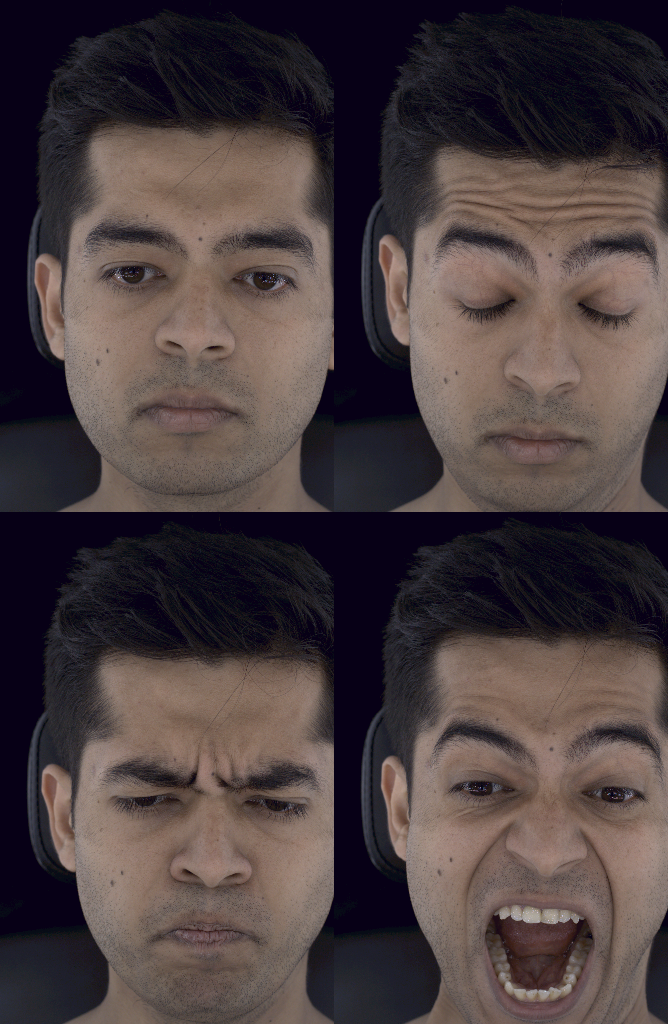
\includegraphics[width=\linewidth,trim={0 2em 0 2em}, clip]{assets/\blendfieldsdirname/rebuttal/frames.png}
  \caption{\textbf{Training frames} -- In~\cref{sec:blendfields-experiments}, we show results for the \blendfields trained on $\nExpr{=}5$ expressions.
    The images represent these expressions for one of the subjects.
    For each subject, we selected similar expressions to show all possible
    wrinkles when combined.
    Please note that we also include a ``neutral'' expression (the first from
    the left)---it is necessary to enable the learning of a face without any
    wrinkles.
    % model to learn 
  }
  \label{fig:blendfields-supplementary-training-frames}
\end{figure}
  \subsection{Training frames}
    We present in~\cref{fig:blendfields-supplementary-training-frames} example
    training frames for one of the subjects.
    Each frame is a multi-view frame captured with ${\approx} 35$ cameras (the
    number of available cameras varied slightly between subjects).

    \begin{table}[!t]
  \centering
  \resizebox{\linewidth}{!}{
    \begin{tabular}{lcccccc}
      \toprule
      \multirow{2}[2]{*}{Method}                         & \multicolumn{3}{c}{Casual Expressions} & \multicolumn{3}{c}{Novel Pose Synthesis}                                                                                                                                                  \\
      \cmidrule(lr){2-4}\cmidrule(lr){5-7}
                                                         & PSNR $\uparrow$                        & SSIM $\uparrow$                          & LPIPS $\downarrow$                & PSNR $\uparrow$                    & SSIM $\uparrow$                   & LPIPS $\downarrow$                \\
      \midrule
      NeRF \cite{mildenhall2020nerf}                     & 22.0060                                & 0.6556                                   & 0.3222                            & 23.8077                            & 0.7448                            & 0.2779                            \\
      Conditioned NeRF \cite{mildenhall2020nerf}         & 21.0846                                & 0.6280                                   & 0.3042                            & 22.9991                            & 0.7261                            & 0.2362                            \\
      NeRFies \cite{park2021nerfies}                     & 20.7004                                & 0.6076                                   & 0.3579                            & 23.0123                            & 0.7253                            & 0.2840                            \\
      HyperNeRF-AP \cite{park2021hypernerf}              & 20.8105                                & 0.6214                                   & 0.3504                            & 22.8193                            & 0.7185                            & 0.2689                            \\
      HyperNeRF-DS \cite{park2021hypernerf}              & 20.8847                                & 0.6111                                   & 0.3656                            & 23.0075                            & 0.7259                            & 0.2729                            \\
      \midrule
      VolTeMorph$_1$ \cite{garbin2024voltemorph}         & 21.3265                                & 0.7091                                   & 0.2706                            & 22.3007                            & 0.7795                            & \cellcolor{secondbestcolor}0.2281 \\
      VolTeMorph$_\text{avg}$\cite{garbin2022voltemorph} & \cellcolor{secondbestcolor}22.0759     & \cellcolor{secondbestcolor}0.7755        & \cellcolor{secondbestcolor}0.2615 & \cellcolor{secondbestcolor}23.8974 & \cellcolor{secondbestcolor}0.8458 & 0.2302                            \\
      \midrule
      \textbf{\methodname{}}                             & \cellcolor{firstbestcolor}22.8982      & \cellcolor{firstbestcolor}0.7954         & \cellcolor{firstbestcolor}0.2256  & \cellcolor{firstbestcolor}24.4432  & \cellcolor{firstbestcolor}0.8477  & \cellcolor{firstbestcolor}0.2052  \\
      \bottomrule
    \end{tabular}
  }
  \caption{\textbf{Quantitative results without masking} --
    Similarly to \cref{tab:blendfields-quantitative-results}, we compare \blendfields to other related approaches.
    However, we calculate the results over the whole image space, without
    removing the background.
    \blendfields and VolTeMorph~\cite{garbin2024voltemorph} model the background as a separate NeRF-based~\cite{mildenhall2020nerf} network.
    The points that do not fall into the tetrahedral mesh are assigned to the
    background.
    As the network overfits to sparse training views, it poorly extrapolates
    to novel expressions (as the new head pose or expression may reveal some
    unknown parts of the background) and views.
    At the same time, all other baselines do not have any mechanism to
    disambiguate the background and the foreground.
  }
  % }
  \label{tab:blendfields-quantitative-results-without-masking}
\end{table}
  \subsection{Quantitative results with background}
    We compare \blendfields and the baselines similarly
    to~\cref{subsec:realistic-human-captures}.
    However, in this experiment, we deliberately include the background in
    metric calculation.
    We show the results in
    \cref{tab:blendfields-quantitative-results-without-masking}.
    In all the cases, \blendfields performs best even though the method was
    not designed to model the background accurately.
    Additionally, as HyperNeRF~\cite{park2021hypernerf},
    NeRFies~\cite{park2021nerfies}, and NeRF~\cite{mildenhall2020nerf} do not
    have any mechanism to disambiguate between the foreground and the
    background, the metrics are significantly worse when including the latter.

  \subsection{Additional qualitative results}

    We show in~\cref{fig:qualitative-other-baselines} results of baselines
    that do not rely on parametric models of the face~\cite{li2017flame}.
    Compared to \blendfields, they cannot render high-fidelity faces.
    The issue comes from the assumed data sparsity---those approaches rely on
    the interpolation in the training data.
    As we assume access to just a few frames, there is no continuity in the
    training data that would guide them to interpolate between known
    expressions.
    \blendfields presents superior results given novel expressions even with such a sparse dataset.
    results.

    \clearpage
    
\renewcommand{\imagewidth}{3.3cm}
\renewcommand{\imageheight}{4.0263671874999996cm}
\renewcommand{\smallimagewidth}{0.8cm}
\renewcommand{\expressionsep}{0em}

\newcommand{\firstindex}{0189}
\newcommand{\secondindex}{0091}
\newcommand{\thirdindex}{0505}
\newcommand{\fourthindex}{0852}

\newcommand{\supimageoneindex}[2]{
  \includegraphics[width=\imagewidth, trim={0 0 0 0}, clip]{assets/\blendfieldsdirname/supplementary/expressions/#1_2183941_selected_rom_#2_\firstindex.png}
}
\newcommand{\supimagetwoindex}[2]{
  \includegraphics[width=\imagewidth, trim={0 0 0 0}, clip]{assets/\blendfieldsdirname/supplementary/expressions/#1_5372021_selected_rom_#2_\secondindex.png}
}
\newcommand{\supimagethreeindex}[2]{
  \includegraphics[width=\imagewidth, trim={0 0 0 0}, clip]{assets/\blendfieldsdirname/supplementary/expressions/#1_6795937_selected_rom_#2_\thirdindex.png}
}
\newcommand{\supimagefourindex}[2]{
  \includegraphics[width=\imagewidth, trim={0 0 0 0}, clip]{assets/\blendfieldsdirname/supplementary/expressions/#1_7889059_selected_rom_#2_\fourthindex.png}
}

\renewcommand{\versionone}{
  \begin{tikzpicture}[
      >=stealth',
      overlay/.style={
          anchor=south west,
          draw=black,
          rectangle,
          line width=0.8pt,
          outer sep=0,
          inner sep=0,
        },
    ]
    \matrix[
      matrix of nodes,
      column sep=0pt,
      row sep=0pt,
      ampersand replacement=\&,
      inner sep=0,
      outer sep=0,
      draw=black,
      rectangle,
      line width=0.5pt
    ] (gt) {
      \supimageoneindex{gt}{0}   \\
      \supimagetwoindex{gt}{0}   \\
      \supimagethreeindex{gt}{0} \\
      \supimagefourindex{gt}{0}  \\
    };

    \matrix[
      matrix of nodes,
      column sep=0pt,
      row sep=0pt,
      ampersand replacement=\&,
      inner sep=0,
      outer sep=0,
      right=0pt of gt-1-1.east,
      draw=black,
      rectangle,
      line width=0.5pt
    ] (k1) {
      \supimageoneindex{bv_aux}{0} \&
      \supimageoneindex{bv_aux}{0-1} \&
      \supimageoneindex{bv_aux}{0-1-2} \&
      \supimageoneindex{bv_aux}{0-1-2-3} \&
      \supimageoneindex{bv_aux}{0-1-2-3-4} \\
    };

    \matrix[
      matrix of nodes,
      column sep=0pt,
      row sep=0pt,
      ampersand replacement=\&,
      inner sep=0,
      outer sep=0,
      right=0pt of gt-2-1.east,
      draw=black,
      rectangle,
      line width=0.5pt
    ] (k2) {
      \supimagetwoindex{bv_aux}{0} \&
      \supimagetwoindex{bv_aux}{0-1} \&
      \supimagetwoindex{bv_aux}{0-1-2} \&
      \supimagetwoindex{bv_aux}{0-1-2-3} \&
      \supimagetwoindex{bv_aux}{0-1-2-3-4} \\
    };

    \matrix[
      matrix of nodes,
      column sep=0pt,
      row sep=0pt,
      ampersand replacement=\&,
      inner sep=0,
      outer sep=0,
      right=0pt of gt-3-1.east,
      draw=black,
      rectangle,
      line width=0.5pt
    ] (k3) {
      \supimagethreeindex{bv_aux}{0} \&
      \supimagethreeindex{bv_aux}{0-1} \&
      \supimagethreeindex{bv_aux}{0-1-2} \&
      \supimagethreeindex{bv_aux}{0-1-2-3} \&
      \supimagethreeindex{bv_aux}{0-1-2-3-4} \\
    };

    \matrix[
      matrix of nodes,
      column sep=0pt,
      row sep=0pt,
      ampersand replacement=\&,
      inner sep=0,
      outer sep=0,
      right=0pt of gt-4-1.east,
      draw=black,
      rectangle,
      line width=0.5pt
    ] (k4) {
      \supimagefourindex{bv_aux}{0} \&
      \supimagefourindex{bv_aux}{0-1} \&
      \supimagefourindex{bv_aux}{0-1-2} \&
      \supimagefourindex{bv_aux}{0-1-2-3} \&
      \supimagefourindex{bv_aux}{0-1-2-3-4} \\
    };

    \node[above=0em of gt-1-1.north, align=center, anchor=south]{Ground Truth};
    \node[above=0em of k1-1-1.north, align=center, anchor=south]{$K={1}$};
    \node[above=0em of k1-1-2.north, align=center, anchor=south]{$K={2}$};
    \node[above=0em of k1-1-3.north, align=center, anchor=south]{$K={3}$};
    \node[above=0em of k1-1-4.north, align=center, anchor=south]{$K={4}$};
    \node[above=0em of k1-1-5.north, align=center, anchor=south]{$K={5}$};

    \node[left=0em of gt-1-1.west, align=center, anchor=east]{\rotatebox{90}{\textsc{Subject} 2183941}};
    \node[above=0em of gt-2-1.west, align=center, anchor=east]{\rotatebox{90}{\textsc{Subject} 5372021}};
    \node[above=0em of gt-3-1.west, align=center, anchor=east]{\rotatebox{90}{\textsc{Subject} 6795937}};
    \node[above=0em of gt-4-1.west, align=center, anchor=east]{\rotatebox{90}{\textsc{Subject} 7889059}};
  \end{tikzpicture}
}

\begin{figure*}[htb]
  \centering
  \resizebox{\linewidth}{!}{
    \versionone
  }
  \caption{\textbf{Qualitative ablation over the number of training expressions} -- {
      We show qualitatively how the number of training expressions $\nExpr$
      affects the rendering quality.
      The first row shows the ground truth images.
      All other consecutive rows show the images rendered with \blendfields
      while increasing the number of training expressions.
      The last row, $\nExpr{=}5$ corresponds to the results presented in the
      main part of the article.
      The subject's naming follows the convention introduced in the Multiface
      repository~\cite{wuu2022multiface}.
      Please refer to~\cref{tab:blendfields-ablation-num-expressions-fix} for
      quantitative results.
    }}
  \label{fig:blendfields-qualitative-ablation-expressions}
\end{figure*}

    
\renewcommand{\imagewidth}{2.7cm}
\renewcommand{\imageheight}{4.0263671874999996cm}
\renewcommand{\smallimagewidth}{0.8cm}
\renewcommand{\expressionsep}{0em}

\renewcommand{\firstindex}{0580}
\renewcommand{\secondindex}{0378}
\renewcommand{\thirdindex}{0226}
\renewcommand{\fourthindex}{0720}

\renewcommand{\supimageoneindex}[1]{
  \includegraphics[width=\imagewidth, trim={0 0 0 0}, clip]{assets/\blendfieldsdirname/supplementary/baselines/#1_2183941_selected_rom_\firstindex.png}
}
\renewcommand{\supimagetwoindex}[1]{
  \includegraphics[width=\imagewidth, trim={0 0 0 0}, clip]{assets/\blendfieldsdirname/supplementary/baselines/#1_5372021_selected_rom_\secondindex.png}
}
\renewcommand{\supimagethreeindex}[1]{
  \includegraphics[width=\imagewidth, trim={0 0 0 0}, clip]{assets/\blendfieldsdirname/supplementary/baselines/#1_6795937_selected_rom_\thirdindex.png}
}
\renewcommand{\supimagefourindex}[1]{
  \includegraphics[width=\imagewidth, trim={0 0 0 0}, clip]{assets/\blendfieldsdirname/supplementary/baselines/#1_7889059_selected_rom_\fourthindex.png}
}

\renewcommand{\versionone}{
  \tikzsetnextfilename{blendfields_other_baselines}
  \begin{tikzpicture}[
      >=stealth',
      overlay/.style={
          anchor=south west,
          line width=0,
          outer sep=0,
          inner sep=0,
        },
    ]
    \matrix[
      matrix of nodes,
      column sep=0pt,
      row sep=0pt,
      ampersand replacement=\&,
      inner sep=0,
      outer sep=0,
      line width=0
    ] (gt) {
      \supimageoneindex{gt}   \\
      \supimagetwoindex{gt}   \\
      \supimagethreeindex{gt} \\
      \supimagefourindex{gt}  \\
    };

    \matrix[
      matrix of nodes,
      column sep=0pt,
      row sep=0pt,
      ampersand replacement=\&,
      inner sep=0,
      outer sep=0,
      right=0pt of gt-1-1.east,
      line width=0,
    ] (k1) {
      \supimageoneindex{bv_aux} \&
      \supimageoneindex{nerf}   \&
      \supimageoneindex{dnerf} \&
      \supimageoneindex{nerfies} \&
      \supimageoneindex{hypernerf_static}    \&
      \supimageoneindex{hypernerf_dynamic} \\
    };

    \matrix[
      matrix of nodes,
      column sep=0pt,
      row sep=0pt,
      ampersand replacement=\&,
      inner sep=0,
      outer sep=0,
      right=0pt of gt-2-1.east,
      line width=0,
    ] (k2) {
      \supimagetwoindex{bv_aux} \&
      \supimagetwoindex{nerf}   \&
      \supimagetwoindex{dnerf} \&
      \supimagetwoindex{nerfies} \&
      \supimagetwoindex{hypernerf_static}    \&
      \supimagetwoindex{hypernerf_dynamic} \\
    };

    \matrix[
      matrix of nodes,
      column sep=0pt,
      row sep=0pt,
      ampersand replacement=\&,
      inner sep=0,
      outer sep=0,
      right=0pt of gt-3-1.east,
      line width=0
    ] (k3) {
      \supimagethreeindex{bv_aux} \&
      \supimagethreeindex{nerf}   \&
      \supimagethreeindex{dnerf} \&
      \supimagethreeindex{nerfies} \&
      \supimagethreeindex{hypernerf_static}    \&
      \supimagethreeindex{hypernerf_dynamic} \\
    };

    \matrix[
      matrix of nodes,
      column sep=0pt,
      row sep=0pt,
      ampersand replacement=\&,
      inner sep=0,
      outer sep=0,
      right=0pt of gt-4-1.east,
      line width=0
    ] (k4) {
      \supimagefourindex{bv_aux} \&
      \supimagefourindex{nerf}   \&
      \supimagefourindex{dnerf} \&
      \supimagefourindex{nerfies} \&
      \supimagefourindex{hypernerf_static}    \&
      \supimagefourindex{hypernerf_dynamic} \\
    };

    \node[above=0em of gt-1-1.north, align=center, anchor=south]{Ground Truth};
    \node[above=0em of k1-1-1.north, align=center, anchor=south]{\textbf{\methodname{}}};
    \node[above=0em of k1-1-2.north, align=center, anchor=south]{NeRF};
    \node[above=0em of k1-1-3.north, align=center, anchor=south]{NeRF+expr};
    \node[above=0em of k1-1-4.north, align=center, anchor=south]{NeRFies};
    \node[above=0em of k1-1-5.north, align=center, anchor=south]{HyperNeRF-AP};
    \node[above=0em of k1-1-6.north, align=center, anchor=south]{HyperNeRF-DS};

    \node[left=0em of gt-1-1.west, align=center, anchor=east]{\rotatebox{90}{\textsc{Subject} 2183941}};
    \node[above=0em of gt-2-1.west, align=center, anchor=east]{\rotatebox{90}{\textsc{Subject} 5372021}};
    \node[above=0em of gt-3-1.west, align=center, anchor=east]{\rotatebox{90}{\textsc{Subject} 6795937}};
    \node[above=0em of gt-4-1.west, align=center, anchor=east]{\rotatebox{90}{\textsc{Subject} 7889059}};
  \end{tikzpicture}
}

\begin{figure*}[htb]
  \centering
  \resizebox{\linewidth}{!}{\versionone}
  \caption{\textbf{Comparison to strictly data-driven approaches} --
    We compare \blendfields to other baselines that do not rely on mesh-driven rendering: NeRF~\cite{mildenhall2020nerf}, NeRF conditioned on the expression code (NeRF+expr)~\cite{mildenhall2020nerf}, NeRFies~\cite{park2021nerfies}, and HyperNeRF-AP/DS~\cite{park2021hypernerf}.
    As a static model, NeRF converges to an average face from available
    ($\nExpr{=}5$) expressions.
    All other baselines exhibit severe artifacts compared to \blendfields.
    Those baselines rely on the data continuity in the training set (\eg, from
    a video), and cannot generalize to any other expression.
  }
  \label{fig:blendfields-qualitative-other-baselines}
\end{figure*}


\chapter{\blendfields: Few-Shot Example-Driven Facial Modeling}
\label{chap:blendfields}
% \newcommand{\blendfieldsdirname}{4_blendfields}

% 
\newcommand{\imagewidth}{2.3cm}
\newcommand{\imageheight}{3.5263671874999996cm}
\newcommand{\smallimagewidth}{0.8cm}
\newcommand{\smallimageheight}{1.2265625cm}
\newcommand{\borderthickness}{0.41pt}
\def\myshift#1{\raisebox{0.5ex}}
\renewcommand{\teasernobox}{
  \begin{subfigure}[b]{\linewidth}
    \centering
    \resizebox{\linewidth}{!}{
      \begin{tikzpicture}[
          >=stealth',
          overlay/.style={
              anchor=south west,
              draw=black,
              rectangle,
              line width=0.8pt,
              outer sep=0,
              inner sep=0,
            },
        ]
        \small
        \matrix[matrix of nodes, column sep=1pt, row sep=1pt, ampersand replacement=\&, inner sep=0, outer sep=0] (training) {
          \includegraphics[height=\imageheight]{assets/\blendfieldsdirname/teaser2/voltemorph/0000_mix.png} \&
          \includegraphics[height=\imageheight]{assets/\blendfieldsdirname/teaser2/voltemorph/0001_mix.png} \&
          \includegraphics[height=\imageheight]{assets/\blendfieldsdirname/teaser2/voltemorph/0003_mix.png} \&
          \includegraphics[height=\imageheight]{assets/\blendfieldsdirname/teaser2/voltemorph/0004_mix.png} \&
          \includegraphics[height=\imageheight]{assets/\blendfieldsdirname/teaser2/voltemorph/0007_mix.png} \\
          \includegraphics[height=\imageheight]{assets/\blendfieldsdirname/teaser2/ours/0000_mix.png} \&
          \includegraphics[height=\imageheight]{assets/\blendfieldsdirname/teaser2/ours/0001_mix.png} \&
          \includegraphics[height=\imageheight]{assets/\blendfieldsdirname/teaser2/ours/0003_mix.png} \&
          \includegraphics[height=\imageheight]{assets/\blendfieldsdirname/teaser2/ours/0004_mix.png} \&
          \includegraphics[height=\imageheight]{assets/\blendfieldsdirname/teaser2/ours/0007_mix.png}       \\
        };
        \node[above right=\borderthickness and \borderthickness of training-2-1.south west, overlay]{
          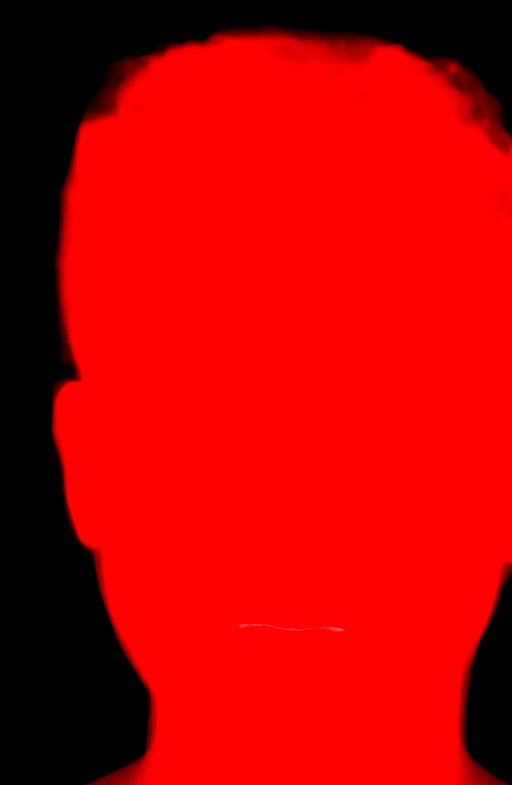
\includegraphics[height=\smallimageheight]{assets/\blendfieldsdirname/teaser2/colorsv2/0000.png}
        };
        \node[above right=\borderthickness and \borderthickness of training-2-2.south west, overlay]{
          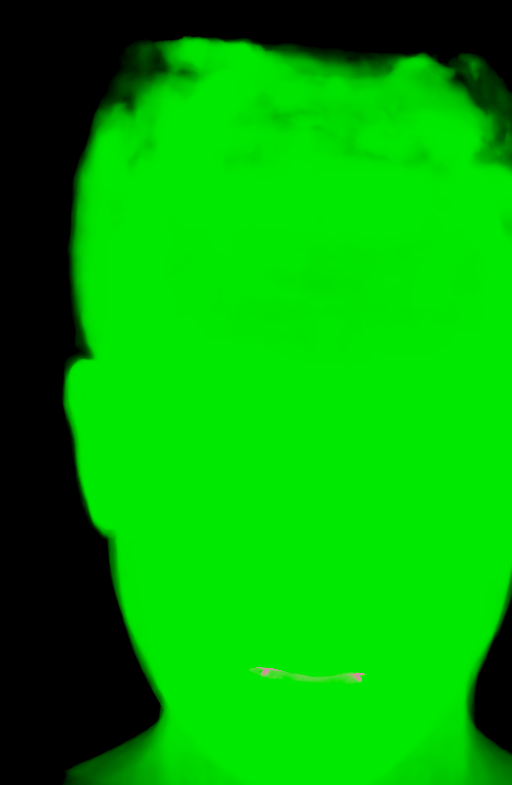
\includegraphics[height=\smallimageheight]{assets/\blendfieldsdirname/teaser2/colorsv2/0001.png}
        };
        \node[above right=\borderthickness and \borderthickness of training-2-3.south west, overlay]{
          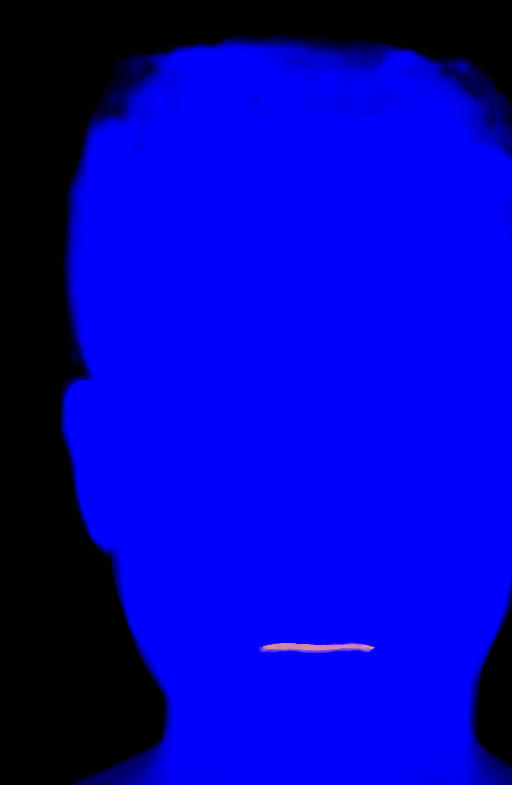
\includegraphics[height=\smallimageheight]{assets/\blendfieldsdirname/teaser2/colorsv2/0002.png}
        };
        \node[above right=\borderthickness and \borderthickness of training-2-4.south west, overlay]{
          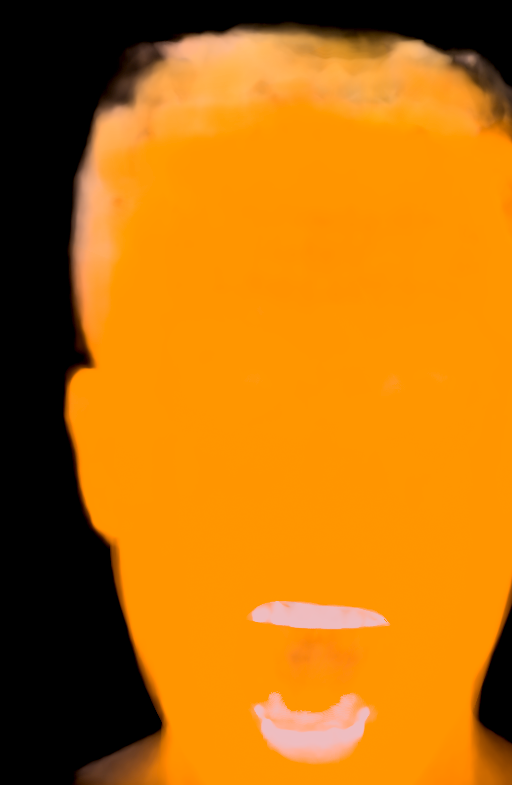
\includegraphics[height=\smallimageheight]{assets/\blendfieldsdirname/teaser2/colorsv2/0003.png}
        };
        \node[above right=\borderthickness and \borderthickness of training-2-5.south west, overlay]{
          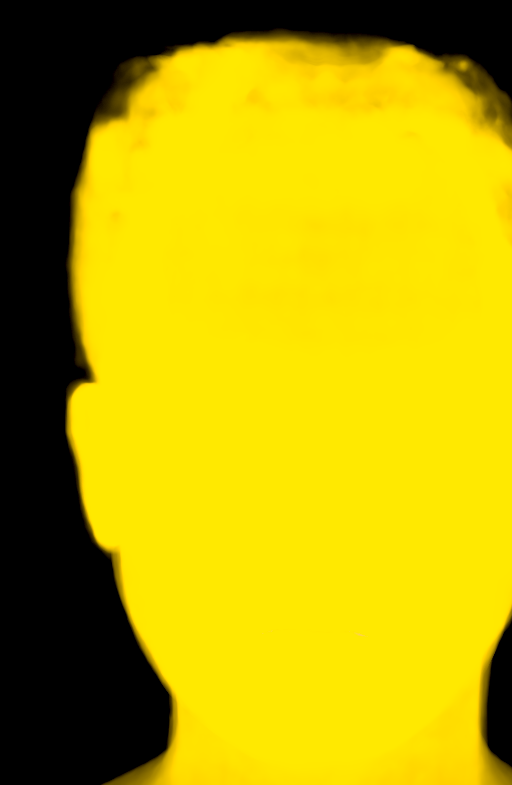
\includegraphics[height=\smallimageheight]{assets/\blendfieldsdirname/teaser2/colorsv2/0004.png}
        };

        \matrix[matrix of nodes, column sep=1pt, row sep=1pt, ampersand replacement=\&, right=1em of training, inner sep=0, outer sep=0] (final) {
          \includegraphics[height=\imageheight]{assets/\blendfieldsdirname/teaser2/voltemorph/final_markings.png} \\
          \includegraphics[height=\imageheight]{assets/\blendfieldsdirname/teaser2/ours/final_markings.png}       \\
        };
        \node[above right=\borderthickness and \borderthickness of final-2-1.south west, overlay]{
          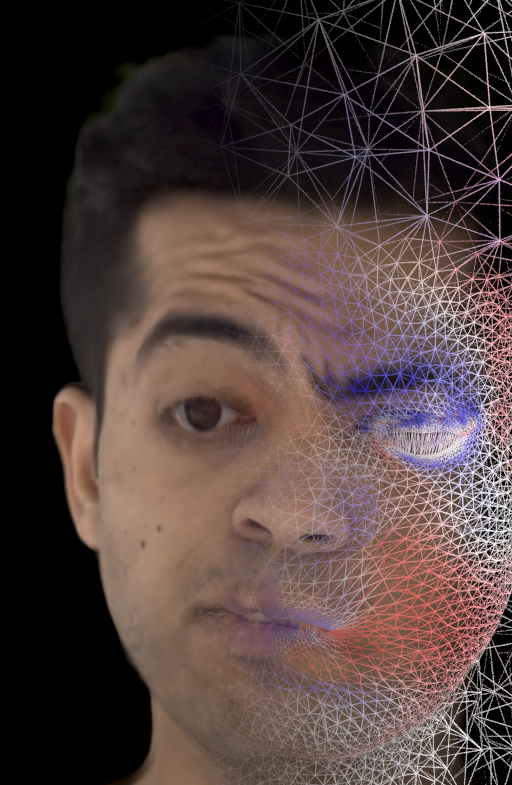
\includegraphics[height=\smallimageheight]{assets/\blendfieldsdirname/teaser2/colorsv2/final.png}
        };
        \node[above right=\borderthickness and \borderthickness of final-1-1.south west, overlay]{
          
\includegraphics[height=\smallimageheight]{assets/\blendfieldsdirname/teaser/colors/voltemorph.png}
        };

        % \node[below=0.25em of final-1-2] {\textbf{Ours}}; \node[below=0.25em
        % of final-1-1] {VolTeMorph \cite{garbin2022voltemorph}};
        % \node[left=0.75em of training-1-1.west, rotate=90, anchor=center]
        % {VolTeMorph \cite{garbin2022voltemorph}};
        \node[left=0.75em of training-1-1.west, rotate=90, anchor=center] {VolTeMorph};
        \node[left=0.75em of training-2-1.west, rotate=90, anchor=center] {\textbf{Ours}};
        % \draw[-] ($(training-1-1.south west)+(0.5em,-0.3em)$) -- node[below]
        % {Rendered training expressions} ($(training-1-5.south
        % east)+(-0.5em,-0.3em)$);
        \node[below=0.25em of training.south] {Rendered training expressions};
        \node[below left=0.25em and -2.5em of final-2-1.south] {Novel expression};

        \draw[densely dotted, line width=0.1em] ($(training-1-5.north east)+(0.5em,0.0em)$) -- ($(training-2-5.south east)+(0.5em,0.0em)$);

        % \matrix[matrix of nodes, inner sep=0, outer sep=0, column sep=0cm,
        % row sep=0cm, ampersand replacement=\&, right=1em of final]
        % (voltemorph) {

        % }; \draw[->,postaction={decorate,decoration={text along path,text
        % align=center,}}] (training-1-5.east) to [out=30,in=150]
        % (final-1-1.west);
      \end{tikzpicture}
    }
    % \includegraphics[width=\linewidth, height=8em]{example-image-a}
  \end{subfigure}
}

\newcommand{\blendfieldsteaserfigure}{
  \begin{figure}
    \centering
    \teasernobox
    \caption{
      \textbf{Teaser} --
      Given five multi-view frames of different expressions, our approach generates a model capable of capturing the fine-grained details of a novel expression beyond the resolution of the underlying face model~\cite{garbin2024voltemorph} (top right corner).
      This is achieved by \textit{blending} the radiance fields computed for
      individual expressions, where the blending coefficients are modulated
      accordingly to \textit{local} volumetric changes.
      These volumetric changes are measured as the difference in the
      tetrahedral volume of a mesh that deforms with the expression
      (\mycoloredbox{seismicred} increase, \mycoloredbox{seismicblue}
      decrease, and \mycoloredbox{seismicgray} no change in volume).
      Such an approach allows \textit{\blendfields} to render sharp,
      expression-dependent details of the face without increasing the
      resolution of the mesh (bottom right corner).
      \label{fig:blendfields-teaser}
    }
  \end{figure}

}
 \blendfieldsteaserfigure

% % \begin{document} \maketitle
% \section{Abstract}
  Decoupling lighting from geometry using unconstrained photo collections is
  notoriously challenging.
  Solving it would benefit many users as creating complex 3D assets takes days
  of manual labor.
  Many previous works have attempted to address this issue, often at the
  expense of output fidelity, which questions the practicality of such
  methods.
  We introduce \lumigauss---a technique that tackles 3D reconstruction of
  scenes and environmental lighting through 2D Gaussian Splatting.
  Our approach yields high-quality scene reconstructions and enables realistic
  lighting synthesis under novel environment maps.
  We also propose a method for enhancing the quality of shadows, common in
  outdoor scenes, by exploiting spherical harmonics properties.
  Our approach facilitates seamless integration with game engines and enables
  the use of fast precomputed radiance transfer.
  We validate our method on the NeRF-OSR dataset, demonstrating superior
  performance over baseline methods.
  Moreover, \lumigauss can synthesize realistic images for unseen environment
  maps.

% \section{Introduction}
  \label{sec:blendfields-intro}

  % --- neural rendering and importance in digital doubles

  Recent advances in neural rendering of 3D scenes~\cite{tewari2022advances}
  offer 3D reconstructions of unprecedented quality~\cite{mildenhall2020nerf}
  with an ever-increasing degree of control ~\cite{kania2022conerf,
  liu2021editing}.
  Human faces are of particular interest to the research
  community~\cite{athar2022rignerf, gafni2021dynamic, garbin2024voltemorph,
  gao2022reconstructing} due to their application in creating realistic
  digital doubles~\cite{ma2021pixel, tewari2022advances, zhang2022avatargen,
  zhi2022dualspace}.

  % --- parametric models cause lack of details
  To render facial expressions not observed during training, current
  solutions~\cite{athar2022rignerf, gafni2021dynamic, garbin2024voltemorph,
  gao2022reconstructing} rely on \textit{parametric} face
  models~\cite{blanz1999morphable}.
  These allow radiance fields~\cite{mildenhall2020nerf} to be controlled by
  facial parameters estimated by off-the-shelf face
  trackers~\cite{li2017flame}.
  However, parametric models primarily capture smooth deformations and lead to
  digital doubles that lack realism because fine-grained and
  expression-dependent phenomena like wrinkles are not faithfully reproduced.
  % \mkc{while this is true, even if wrinkles were modelled by the 3dmm, they
  % would not appear,as nerfs do not model illumination and wrinkles are only
  % visible thanis to shadows} --- how this problem is addressed for now (DATA)
  % \at{

  Authentic Volumetric Avatars (AVA)~\cite{cao2022authentic} overcomes this
  issue by learning from a large multi-view dataset of synchronized and
  calibrated images captured under controlled lighting.
  Their dataset covers a series of dynamic facial expressions and multiple
  subjects.
  However, this dataset remains unavailable to the public and is expensive to
  reproduce.
  Additionally, training models from such a large amount of data requires
  significant compute resources.
  To democratize digital face avatars, more efficient solutions in terms of
  hardware, data, and compute are necessary.

  % --- What we do (high level) \at{
  We address the efficiency concerns by building on the recent works in Neural
  Radiance Fields~\cite{garbin2024voltemorph,xu2022deforming,yuan2022nerf}.
  % VolTeMorph~\cite{garbin2022voltemorph}.
  In particular, we extend VolTeMorph~\cite{garbin2024voltemorph} to render
  facial details learned from images of a sparse set of expressions.
  To achieve this, we draw inspiration from blend-shape
  correctives~\cite{lewis2014practice}, which are often used in computer
  graphics as a data-driven way to correct potential mismatches between a
  simplified model and the complex phenomena it aims to represent.
  In our setting, this mismatch is caused by the low-frequency deformations
  that the tetrahedral mesh from VolTeMorph~\cite{garbin2024voltemorph},
  designed for real-time performance, can capture, and the high-frequency
  nature of expression \mbox{wrinkles}.

  % --- what we do (low level) \at{
  We train multiple radiance fields, one for each of the $\nExpr$ sparse
  expressions present in the input data, and blend them to correct the
  low-frequency estimate provided by VolTeMorph~\cite{garbin2024voltemorph};
  see \cref{fig:blendfields-teaser}.
  % Hence, 
  We call our method \blendfields since it resembles the way blend shapes are
  employed in 3DMMs~\cite{blanz1999morphable}.
  To keep $\nExpr$ small (\ie, to maintain a few-shot regime), we perform
  local blending to exploit the known correlation between wrinkles and changes
  in local differential properties~\cite{irving2004invertible, raman2022mesh}.
  Using the dynamic geometry of~\cite{garbin2024voltemorph}, local changes in
  differential properties can be easily extracted by analyzing the tetrahedral
  representation underlying the corrective blendfields of our model.
  % underlying used to train and drive the }

  % --- contributions \at{
  \paragraph{Contributions}
    We outline the main qualitative differences between our approach and
    related works in \cref{tab:blendfields-ava-ours-comparison}, and our
    empirical evaluations confirm these advantages.
    In summary, we:
    \begin{itemize}
      \item extend VolTeMorph~\cite{garbin2024voltemorph} to enable modeling of high-frequency information, such as expression wrinkles in a few-shot setting;
      \item introduce correctives~\cite{blanz1999morphable} to neural field representations and activate them according to local deformations~\cite{raman2022mesh};
      \item
            make this topic more accessible
            with an alternative to techniques that are data and compute-intensive~\cite{cao2022authentic};
      \item show that our model generalizes beyond facial modeling, for example, in the modeling of wrinkles on a deformable object made of rubber.
    \end{itemize}
    \begin{table*}[!t]
  \centering
  \resizebox{\linewidth}{!}{
    \begin{tabular}{lccccccc|c}
      \toprule
                                 & NeRF~\cite{mildenhall2020nerf} & NeRFies~\cite{park2021nerfies} & HyperNeRF~\cite{park2021hypernerf} & NeRFace~\cite{gafni2021dynamic} & NHA~\cite{grassal2022neural} & AVA \cite{cao2022authentic} & VolTeMorph~\cite{garbin2024voltemorph} & \textbf{Ours} \\
      \midrule
      Applicability beyond faces & \cmark                         & \cmark                         & \cmark                             & \xmark                          & \xmark                       & \xmark                      & \cmark                                 & \cmark        \\
      Interpretable control      & \xmark                         & \xmark                         & \xmark                             & \cmark                          & \cmark                       &
      \xmark                     & \cmark                         & \cmark                                                                                                                                                                                                                      \\ Data efficiency & \xmark & \cmark & \cmark &
      \xmark                     & \cmark                         & \xmark                         & \cmark                             & \cmark                                                                                                                                                \\ Expression-dependent
      changes                    & \xmark                         & \xmark                         & \cmark                             & \cmark                          & \cmark                       & \cmark                      & \xmark                                 &
      \cmark                                                                                                                                                                                                                                                                                    \\ Generalizability to unknown expressions & \xmark & \xmark &
      \xmark                     & \cmark                         & \cmark                         & \xmark                             & \cmark                          & \cmark                                                                                                              \\
      \bottomrule\end{tabular} }
  \caption{\textbf{Comparison} -- We compare
    several methods to our approach.
    Other methods fall short in data efficiency and applicability.
    For example, AVA~\cite{cao2022authentic} requires 3.1 million training
    images while VolTeMorph \cite{garbin2024voltemorph} cannot model
    expression-dependent wrinkles realistically.
  }
  \label{tab:blendfields-ava-ours-comparison}
\end{table*}
% \section{Related works}
  \label{sec:conerf-related}
  Neural Radiance Fields~\cite{mildenhall2020nerf} provide high-quality
  renderings of scenes from novel views with just a few exemplar images
  captured by a handheld device.
  Various extensions have been suggested to date.
  These include ones that focus on improving the quality of
  results~\cite{martin2021nerf, park2020deformable, park2021hypernerf,
  zhang2020nerf++}, ones that allow a single model to be used for multiple
  scenes~\cite{schwarz2020graf, trevithick2020grf}, and some considering
  controllability of the rendering output at a coarse
  level~\cite{guo2020object, yu2021unsupervised, liu2021editing,
  yang2021learning, xie2021fig, zhang2021nerfactor}, as we detail next.

  In more detail, existing works enable only compositional control of object
  location~\cite{yang2021learning,yu2021unsupervised}, and recent extensions
  also allow for finer-grain reproduction of global illumination
  effects~\cite{guo2020object}.
  NeRFactor~\cite{zhang2021nerfactor} shows one can model albedos and BRDFs,
  and shadows, which can be used to, \eg, edit material, but the manipulation
  they support is limited to what is modeled through the rendering equation.
  CodeNeRF~\cite{jang2021codenerf} and EditNeRF~\cite{liu2021editing} showed
  that one can edit NeRF models by modifying the shape and appearance
  encoding, but they require a curated dataset of objects viewed under
  different views and colors.
  HyperNeRF~\cite{park2021hypernerf}, on the other hand can adapt to unseen
  changes specific to the scene, but learns an arbitrary attribute (ambient)
  space that cannot be supervised, and, as we show in
  \cref{sec:conerf-results}, cannot be easily related to specific local
  attribute within the scene for controllability.

  \paragraph{Explicit supervision}
    One can also condition NeRF representations~\cite{gafni2021dynamic} with
    face attribute predicted by pre-trained face tracking networks, such as
    Face2Face~\cite{thies2016face2face}.
    Similarly, for human bodies, A-NeRF~\cite{su2021anerf} and
    NARF~\cite{noguchi2021neural} use the SMPL~\cite{loper2015smpl} model to
    generate interpretable pose parameters, and
    Neural~Actor~\cite{liu2021neural} further includes normal and texture maps
    for more detailed rendering.
    While these models result in controllable NeRF, they are limited to
    domain-specific control and the availability of a heavily engineered
    control model.

  \paragraph{Controllable neural implicits}
    Controllability of neural 3D \textit{implicit} representations has also
    been addressed by the research community.
    Many works have limited focus on learning \textit{human} neural implicit
    representations while enabling the control via SMPL
    parameters~\cite{loper2015smpl}, or linear blend skinning
    weights~\cite{zheng2021pamir, he2021arch++, saito2021scanimate,
    mihajlovic2021leap, ma2021scale, deng2020nasa, alldieck2021imghum,
    zins2021data}.
    Some initial attempts at learned disentangled of shape and poses have also
    been made in A-SDF~\cite{mu2021sdf}, allowing behavior control of the
    output geometry~(\eg doors open vs.
    closed) while maintaining the general shape.
    However, the approach is limited to controlling $\text{SE}(3)$
    articulation of objects, and requires dense 3D supervision.
  \subsection{Neural Radiance Field (NeRF)}
    For completeness, we briefly discuss NeRF before diving into the details
    of our method.
    A Neural Radiance Field captures a volumetric representation of a specific
    scene within the weights of a neural network.
    As input, it receives a sample position~$\bx$ and a view direction~$\bv$
    and outputs the density of the scene $\sigma$ at position~$\bx$ as well as
    the color~$\bc$ at position~$\bx$ as seen from view direction~$\bv$.
    One then renders image pixels~$\bC$ via volume
    rendering~\cite{kajiya1984ray}.
    In more detail, $\bx$ is defined by observing rays~$\br(t)$ as
    \mbox{$\bx=\br(t)$}, where $t$ parameterizes at which point of the ray you
    are computing for.
    One then renders the color of each pixel $\bC(\br)$ by computing
    \begin{equation}
      \bC\left(\br\right) = \int_{t_n}^{t_f} T(t) \sigma\left(\br(t)\right) \bc\left(\br(t), \bv\right) dt
      \;,
      \label{eq:conerf-volume_render}
    \end{equation}
    where $\bv$ is the viewing angle of the ray $\br$, $t_n$ and $t_f$ are the near and far planes of the rendering volume, and
    \begin{equation}
      T(t) = \exp \left ( - \int_{t_n}^t \sigma({\bf r}(s)) ds \right ) \;,
      \end{equation} is the accumulated transmittance.
    Integration in \cref{eq:conerf-volume_render} is typically done via
    numerical integration~\cite{mildenhall2020nerf}.

  \subsection{HyperNeRF}
    Note that in its original formulation~\cref{eq:conerf-volume_render} is
    only able to model \textit{static} scenes.
    Various recent works~\cite{park2020deformable, park2021hypernerf,
    tretschk2021non} have been proposed to explicitly account for possible
    appearance changes in a scene (for example, temporal changes in a video).
    To achieve this, they introduce the notion of \textit{canonical} \textit{hyperspace} -- more formally given a 3D query point $\bx$ and the collection $\pars$ of all parameters that describe the model, they define:
    \begin{align}
      \Canonicalizer(\bx)         & \equiv \Canonicalizer(\bx \given \bbeta, \pars ), \quad                 & \text{Canonicalizer} \label{eq:conerf-canonicalizer} \\
      \bbeta(\bx)                 & \equiv \hypermap (\bx \given \bbeta, \pars ), \quad                     & \text{Hyper~Map} \label{eq:conerf-hypermap}          \\
      \bc(\point), \sigma(\point) & = \Representation(\Canonicalizer(\bx), \bbeta(\bx) \given \pars). \quad & \text{Hyper~NeRF}
      \label{eq:conerf-hypernerf}
    \end{align}
    where the location is canonicalized via a canonicalizer $\Canonicalizer$, and the appearances, represented by $\bbeta$, are mapped to a hyperspace via $\hypermap$, which are then utilized by another neural network $\Representation$ to retrieve the color $\bc$ and the density $\sigma$ at the query location.
    Note throughout this paper we denote $\latent$ to indicates a latent code,
    while $\latent(\point)$ to indicate the corresponding field generated by
    the hypermap lifting.
    With this latent lifting, these methods render the scene via
    \cref{eq:conerf-volume_render}.
    Note that the original NeRF model can be thought of the case where
    $\Canonicalizer$ and $\hypermap$ are identity mappings.


% \begin{figure}
  \centering
  \begin{subfigure}[b]{0.39\linewidth}
    \centering
    \includegraphics[width=\linewidth]{fig/\conerfdirname/assets/implicit.pdf}
    \vspace{0.0em}
    \caption{Neural radiance field with lifting~\cite{park2021hypernerf}}
    \label{fig:conerf-implicit}
  \end{subfigure}
  \hfill
  \begin{subfigure}[b]{0.60\linewidth}
    \centering
    \includegraphics[width=\linewidth]{fig/\conerfdirname/assets/lac.pdf}
    \caption{Controllable neural radiance field (our method)}
    \label{fig:conerf-laced-implicit}
  \end{subfigure}
  \vspace{-0.7em}
  \caption{{\bf Framework -- }
    We depict in (a) the HyperNeRF~\cite{park2021hypernerf} formulation, and
    (b) our Controllable-NeRF~(CoNeRF).
    In (a), both point coordinates $\mathbf{x}$ and latent representation
    $\boldsymbol{\beta}$ are respectively processed by a canonicalizer
    $\Canonicalizer$ and a hyper map $\hypermap$, which are then turned into
    radiance and density field values by $\Representation$.
    In (b), we introduce regressors $\Attribute$ and $\MaskNet$ that regress
    the attribute and the corresponding mask that enable few-shot
    attribute-based control of the NeRF model.
    See~\cref{sec:conerf-inference} for details.
  }
  \label{fig:conerf-pipeline}
\end{figure}
\section{Controllable NeRF (CoNeRF)}
  Given a collection of $\nImages$ color images $\images \in [0,1]^{\width \times \height \times 3}$, we train our controllable neural radiance field model by an auto-decoding optimization~\cite{park2019deepsdf} whose losses can be grouped into two main subsets:
  \begin{align}
    \argmin_{\allpars=\pars, \latents}
    \underbrace{\loss{rep}(\allpars \given \images)}_\text{\cref{sec:conerf-autodecode}}{+}
    \underbrace{\loss{ctrl}(\allpars \given
      \{\Mask^\gt_{\iImage, \iAttribute} \}, \{\attribute^\gt_{\iImage,\iAttribute}\} )}_\text{\cref{sec:conerf-control}}
    .
  \end{align}
  The first group consists of the classical HyperNeRF~\cite{park2021hypernerf} auto-decoder losses, attempting to optimize neural network parameters $\pars$ jointly with latent codes $\latents$ to \textit{reproduce} the corresponding input images $\images$:
  \begin{align}
    \loss{rep}(\cdot) =
    \loss{recon}(\pars, \latents \given \images) +
    \loss{enc}(\latents)
    .
    \label{eq:conerf-loss_render}
  \end{align}
  The latter allow us to inject \textit{explicit control} into the representation, and are our core contribution:
  \begin{align}
    \loss{ctrl}(\cdot)
     & = \loss{mask}(\pars, \latents \given \{\Mask^\gt_{\iImage, \iAttribute} \})     & \text{g.t. masks}      \\
     & + \loss{attr}(\pars, \latents \given \{\attribute^\gt_{\iImage,\iAttribute}\}). & \text{g.t. attributes}
    \label{eq:loss_control}
  \end{align}
  As mentioned earlier in \cref{sec:conerf-intro}, we aim for a neural 3D
  appearance model that is controlled by a collection of attributes
  $\attributes {=} \{\attribute_\iAttribute\}$, and we expect each image to be
  a manifestation of a different value of attributes, that is, each image
  $\image_\iImage$, and hence each latent code $\latent_\iImage$, will have a
  corresponding attribute~$\attributes_\iImage$.
  The learnable connection between latent codes $\latent$ and the attributes
  $\attributes$, which we represent via regressors, is detailed
  in~\cref{sec:conerf-inference}.

  \subsection{Reconstruction losses}
    \label{sec:conerf-autodecode}
    The primary loss guiding the training of the NeRF model is the
    reconstruction loss, which simply aims to reconstruct observations
    $\images$.
    As in other neural radiance field models~\cite{mildenhall2020nerf, martin2021nerfw, park2020deformable, park2021hypernerf} we simply minimize the L2 photometric reconstruction error with respect to ground truth images:
    \begin{equation}
      \loss{recon}(\cdot) = \sum_\iImage \expect_{\ray \sim \image_\iImage} \left[ \left\|\bC(\ray \given \latent_\iImage, \pars)-\bC^\text{gt}(\ray) \right\|_2^2 \right]
      .
      \label{eq:conerf-recon}
    \end{equation}
    As is typical in auto-decoders, and following~\cite{park2019deepsdf}, we impose a zero-mean Gaussian prior on the latent codes~$\latents$:
    \begin{equation}
      \loss{enc}(\cdot) = \sum_\iImage \left\| \latent_\iImage \right\|^2_2
      .
      \label{eq:conerf-latent_prior}
    \end{equation}

  \subsection{Control losses}
    \label{sec:conerf-control}
    The user defines a \textit{discrete} set of $\nAttributes$ number of
    attributes that they seek to control, that are \textit{sparsely}
    supervised across frames---we only supervise attributes \textit{when} we
    have an annotation, and let others be discovered on their own throughout
    the training process, as guided by~\cref{eq:conerf-loss_render}.
    More specifically, for a particular image $\image_\iImage$, and a particular attribute $\attribute_\iAttribute$, the user specifies the quantities:
    \begin{itemize}
      \item $\attribute_{\iImage, \iAttribute} \in [-1,1]$: specifying the value for the $\iAttribute$-th attribute in the $\iImage$-th image; see the \textit{sliders} in~\cref{fig:conerf-teaser};
      \item $\Mask_{\iImage, \iAttribute} \in [0,1]^{\width \times \height}$: roughly specifying the image region that is controlled by the $\iAttribute$-th attribute in the $\iImage$-th image; see the \textit{masks} in~\cref{fig:conerf-teaser}.
    \end{itemize}
    To formalize sparse supervision, we employ an indicator function
    $\indicator_{\iImage, \iAttribute}$, where $\indicator_{\iImage,
    \iAttribute}=1$ if an annotation for attribute $\iAttribute$ for image
    $\iImage$ is provided, otherwise $\indicator_{\iImage, \iAttribute}=0$.
    We then write the loss for \textit{attribute} supervision as:
    \begin{equation}
      \loss{attr}(\cdot) =
      \sum_\iImage \sum_\iAttribute
      \indicator_{\iImage, \iAttribute}
      |\attribute_{\iImage,\iAttribute} - \attribute^\gt_{\iImage,\iAttribute}|^2
      .
    \end{equation}

    For the mask few-shot supervision, \
    we employ the volume rendering in~\cref{eq:conerf-volren} to project the 3D volumetric neural mask field $\mask_\iAttribute(\bx)$ into image space, and then supervise it as:
    \newcommand{\crossentropy}[2]{\text{CE}\left(#1,#2\right)}
    \begin{equation}
      \loss{mask}(\cdot) \!= \!\!\sum_{\iImage, \iAttribute}
      \indicator_{\iImage, \iAttribute} \:
      \expect_\ray
      \left[
        \crossentropy
        {\Mask(\ray \given \latent_\iImage, \pars)}
        {\Mask^\gt_{\iImage, \iAttribute}(\ray)}
        \right]
      ,
      \label{eq:conerf-mask}
    \end{equation}
    where $\crossentropy{\cdot}{\cdot}$ denotes cross entropy, and the field $\sigma(\bx)$ in~\cref{eq:conerf-volren} is learned by minimizing~\cref{eq:conerf-recon}.
    Importantly, as we do not wish for~\cref{eq:conerf-mask} to interfere with
    the training of the underlying 3D representation learned through
    \cref{eq:conerf-recon}, we \textit{stop gradients}
    in~\cref{eq:conerf-mask} w.r.t. $\sigma(\bx)$.
    Furthermore, in practice, because the attribute mask vs.
    background distribution can be highly imbalanced depending on which attribute the user is trying to control (\eg an eye only covers a very small portion of an image), we employ a \textit{focal loss}~\cite{lin2017focal} in place of the standard cross entropy loss.

  \subsection{Controlling and rendering images}
    \label{sec:conerf-inference}
    In what follows, we drop the image subscript $\iImage$ to simplify
    notation without any loss of generality.
    Given a $B$-dimensional latent code $\latent$ representing the 3D scene behind an image, we derive a mapping to our $A$ attributes via a neural map $\Attribute$ with learnable parameters $\pars$:
    \begin{equation}
      \{ \attribute_\iAttribute \} = \AttributeNet(\latent \given \pars), \quad
      \AttributeNet : \real^\latentDim \rightarrow [0,1]^\nAttributes
      ,
    \end{equation}
    where these correspond to the \textit{sliders} in~\cref{fig:conerf-teaser}.
    In the same spirit of~\cref{eq:conerf-hypermap}, to allow for complex
    topological changes that may not be represented by the change in a single
    scalar value alone, we lift the attributes to a hyperspace.
    In addition, since each attribute governs different aspects of the scene, we employ \textit{per-attribute} learnable hypermaps $\{\hypermap_\iAttribute\}$, which we write:
    \begin{align}
      \attribute_\iAttribute(\point) & = \hypermap_\iAttribute(\point, \attribute_\iAttribute \given \pars) \quad \hypermap_\iAttribute: \real^3 \times \real \rightarrow \real^\hyperAttributeDim
      .
    \end{align}
    Note that while $\attribute_\iAttribute$ is a scalar \textit{value},
    $\attribute_\iAttribute(\point)$ is a \textit{field} that can be queried
    at any point $\point$ in space.
    These fields are concatenated to form
    $\attributes(\point)=\{\attribute_\iAttribute(\point)\}$.

    We then provide all this information to generate an \textit{attribute
    masking field} via a network $\MaskNet(\cdot \given \pars)$.
    This field determines which attribute \textit{attends} to which position in space~$\point$:
    \begin{align}
      \label{eq:conerf-mask_c}
      \mask_0(\point) & \oplus \mask(\point) = \MaskNet(\Canonicalizer(\point), \bbeta(\point), \attributes(\point) \given \pars),                   \\
      \MaskNet        & : \real^3 \times \real^\latentDim \times \real^{\nAttributes \times \hyperAttributeDim} \rightarrow \real^{\nAttributes+1}_+
      ,
    \end{align}
    where $\oplus$ is a concatenation operator, $\mask(\point){=}\{\mask_\iAttribute(\point)\}$, and the additional mask $\mask_0(\point)$ denotes space that is not affected by \textit{any} attribute.
    Note that because the mask location should be affected by both the
    particular attribute of interest (\eg, the selected eye status) and the
    global appearance of the scene (\eg, head movement), $\MaskNet$ takes both
    $\bbeta(\point)$ and $\attributes(\point)$ as input in addition to
    $\Canonicalizer(\point)$.
    In addition, because the mask is modeling the attention related to attributes, collectively, these masks satisfy the partition of unity property:
    \begin{align}
      \mask_0(\point) + \Sigma_\iAttribute [\mask_\iAttribute(\point)] = 1 \quad \forall \point \in \real^3
      .
    \end{align}
    Finally, in a similar spirit to~\cref{eq:conerf-hypernerf}, all of this information is processed by a neural network that produces the desired radiance and density fields used in volume rendering:
    \begin{equation}
      \begin{rcases}
        \bc(\point) \\
        \sigma(\point)
      \end{rcases} \!\!=\! \Representation(\Canonicalizer(\point),
      \underbrace{\mask(\point) \odot \attributes(\point)}_\text{attribute controls},
      \underbrace{\mask_0(\point) \cdot \latent(\point)}_\text{everything else}
      \given \pars)
      .
      \label{eq:conerf-representation}
    \end{equation}
    In particular, note that $\mask(\point){=}0$ implies
    $\mask_0(\point){=}1$, hence our solution has the capability of reverting
    to classical HyperNeRF~\cref{eq:conerf-hypernerf}, where all change in the
    scene is globally encoded in $\bbeta(\point)$.
    Finally, these fields can be used to render the mask in image space, following a process analogous to volume rendering of radiance:
    \begin{equation}
      \Mask(\ray\given\allpars) \!=\!\!
      \int_{t_n}^{t_f} \!\!\!\!
      T(t) \cdot \sigma(\br(t)) \cdot [\mask_0(\ray(t)) \oplus \mask(\ray(t))]
      \, dt .
      \label{eq:conerf-volren}
    \end{equation}
    We depict our inference flow in~\cref{fig:conerf-pipeline}~(b).

  \subsection{Implementation details}
    We implement our method for NeRF based on the JAX \cite{jax2018github}
    implementation of HyperNeRF~\cite{park2021hypernerf}.
    We use both the scheduled windowed positional encoding and weight
    initialization of \cite{park2020deformable}, as well as the coarse-to-fine
    training strategy~\cite{park2021hypernerf}.

    Besides the newly added networks, we follow the same architecture as
    HyperNeRF.
    For the attribute network $\Attribute$ we use a six-layer multi-layer
    perceptron (MLP) with 32 neurons at each layer, with a skip connection at
    the fifth layer, following \cite{park2020deformable,park2021hypernerf}.
    For the lifting network $\hypermap_\iAttribute$, we use the same
    architecture as $\hypermap$, except for the input and output dimension
    sizes.
    For the masking network $\MaskNet$ we use a four-layer MLP with 128
    neurons at each layer, followed by an additional 64 neuron layer with a
    skip connection.
    The network $\Representation$ also shares the same architecture as
    HyperNeRF, but with a different input dimension size to accommodate for
    the changes our method introduces.

    \paragraph{2D implementation}
      To show that our idea is not limited to neural radiance fields, we also
      test a 2D version of our framework that can be used to directly
      represent images, without going through volume rendering.
      We use the same architecture and training procedure as in the NeRF case,
      with the exception that we do not predict the density $\sigma$, and we
      also do not have the notion of depth---each ray is directly the pixel.
      We center crop each video and resize each frame to be $128\times128$.

    \paragraph{Hyperparameters}
      We train all our NeRF models with $480\times270$ images and with 128
      samples per ray.
      We train for 250k iterations with a batch size of 512 rays.
      During training, we maintain that 10\% of rays are sampled from
      annotated images.
      We set $\loss{attr}=10^{-1}$, $\loss{mask}=10^{-2}$ and
      $\loss{enc}=10^{-4}$.
      For the number of hyper dimensions we set $\hyperAttributeDim = 8$.
      For the 2D implementation experiments, we sample 64 random images from
      the scene and further subsample 1024 pixels from each of them.
      For all experiments we use Adam~\cite{kingma2014adam} with learning rate
      $10^{-4}$ exponentially decaying to $10^{-5}$ in 250k iterations.
      We provide additional details in the supplementary material.
      Training a single model takes around 12 hours on an NVIDIA V100 GPU.

% % \renewcommand{\imagewidth}{2.3cm}
\renewcommand{\imageheight}{4.5263671874999996cm}
\renewcommand{\smallimagewidth}{0.8cm}

\newcommand{\imageoneindex}[2]{
  \includegraphics[height=\imageheight, trim={0.7cm 1.8cm 0.7cm 0}, clip]{assets/\blendfieldsdirname/qualitative/extrapolation/#1_6795937_extrapolation_#2.png}
}
\newcommand{\imagetwoindex}[2]{
  \includegraphics[height=\imageheight, trim={1.4cm 1.8cm 0 0}, clip]{assets/\blendfieldsdirname/qualitative/extrapolation/#1_7889059_extrapolation_#2.png}
}
\renewcommand{\versionone}{
  \tikzsetnextfilename{blendfields_qualitative_comparison_extrapolation}
  \begin{tikzpicture}[
      >=stealth',
      overlay/.style={
          anchor=south west,
          draw=black,
          rectangle,
          line width=0.8pt,
          outer sep=0,
          inner sep=0,
        },
    ]
    \matrix[
      matrix of nodes,
      column sep=0pt,
      row sep=0pt,
      ampersand replacement=\&,
      inner sep=0,
      outer sep=0
    ] (nerf) {
      \imageoneindex{nerf}{0000} \\
      % \imageoneindex{nerf}{0002} \\
      \imageoneindex{nerf}{0004} \\

      \imagetwoindex{nerf}{0000} \\
      % \imagetwoindex{nerf}{0002} \\
      \imagetwoindex{nerf}{0004} \\
    };

    \matrix[
      matrix of nodes,
      column sep=0pt,
      row sep=0pt,
      ampersand replacement=\&,
      inner sep=0,
      outer sep=0,
      right=1pt of nerf
    ] (dnerf) {
      \imageoneindex{dnerf}{0000} \\
      % \imageoneindex{dnerf}{0002} \\
      \imageoneindex{dnerf}{0004} \\

      \imagetwoindex{dnerf}{0000} \\
      % \imagetwoindex{dnerf}{0002} \\
      \imagetwoindex{dnerf}{0004} \\
    };

    \matrix[
      matrix of nodes,
      column sep=0pt,
      row sep=0pt,
      ampersand replacement=\&,
      inner sep=0,
      outer sep=0,
      right=1pt of dnerf
    ] (nerfies) {
      \imageoneindex{nerfies}{0000} \\
      % \imageoneindex{nerfies}{0002} \\
      \imageoneindex{nerfies}{0004} \\

      \imagetwoindex{nerfies}{0000} \\
      % \imagetwoindex{nerfies}{0002} \\
      \imagetwoindex{nerfies}{0004} \\
    };

    \matrix[
      matrix of nodes,
      column sep=0pt,
      row sep=0pt,
      ampersand replacement=\&,
      inner sep=0,
      outer sep=0,
      right=1pt of nerfies
    ] (hypernerfstatic) {
      \imageoneindex{hypernerf_static}{0000} \\
      % \imageoneindex{hypernerf_static}{0002} \\
      \imageoneindex{hypernerf_static}{0004} \\

      \imagetwoindex{hypernerf_static}{0000} \\
      % \imagetwoindex{hypernerf_static}{0002} \\
      \imagetwoindex{hypernerf_static}{0004} \\
    };

    \matrix[
      matrix of nodes,
      column sep=0pt,
      row sep=0pt,
      ampersand replacement=\&,
      inner sep=0,
      outer sep=0,
      right=1pt of hypernerfstatic
    ] (hypernerfdynamic) {
      \imageoneindex{hypernerf_dynamic}{0000} \\
      % \imageoneindex{hypernerf_dynamic}{0002} \\
      \imageoneindex{hypernerf_dynamic}{0004} \\

      \imagetwoindex{hypernerf_dynamic}{0000} \\
      % \imagetwoindex{hypernerf_dynamic}{0002} \\
      \imagetwoindex{hypernerf_dynamic}{0004} \\
    };

    \matrix[
      matrix of nodes,
      column sep=0pt,
      row sep=0pt,
      ampersand replacement=\&,
      inner sep=0,
      outer sep=0,
      right=1pt of hypernerfdynamic
    ] (voltemorphstatic) {
      \imageoneindex{voltemorph_static}{0000} \\
      % \imageoneindex{voltemorph_static}{0002} \\
      \imageoneindex{voltemorph_static}{0004} \\

      \imagetwoindex{voltemorph_static}{0000} \\
      % \imagetwoindex{voltemorph_static}{0002} \\
      \imagetwoindex{voltemorph_static}{0004} \\
    };

    \matrix[
      matrix of nodes,
      column sep=0pt,
      row sep=0pt,
      ampersand replacement=\&,
      inner sep=0,
      outer sep=0,
      right=1pt of voltemorphstatic
    ] (voltemorph) {
      \imageoneindex{voltemorph}{0000} \\
      % \imageoneindex{voltemorph}{0002} \\
      \imageoneindex{voltemorph}{0004} \\

      \imagetwoindex{voltemorph}{0000} \\
      % \imagetwoindex{voltemorph}{0002} \\
      \imagetwoindex{voltemorph}{0004} \\
    };

    \matrix[
      matrix of nodes,
      column sep=0pt,
      row sep=0pt,
      ampersand replacement=\&,
      inner sep=0,
      outer sep=0,
      right=1pt of voltemorph
    ] (ours) {
      \imageoneindex{blendvolumes_aux}{0000} \\
      % \imageoneindex{blendvolumes_aux}{0002} \\
      \imageoneindex{blendvolumes_aux}{0004} \\

      \imagetwoindex{blendvolumes_aux}{0000} \\
      % \imagetwoindex{blendvolumes_aux}{0002} \\
      \imagetwoindex{blendvolumes_aux}{0004} \\
    };
    \node[above=0.2em of nerf-1-1.north, align=center, anchor=south]{NeRF};
    \node[above=0.2em of dnerf-1-1.north, align=center, anchor=south]{Conditioned NeRF};
    \node[above=0.2em of nerfies-1-1.north, align=center, anchor=south]{NeRFies};
    \node[above=0.0em of hypernerfstatic-1-1.north, align=center, anchor=south]{HyperNeRF-AP};
    \node[above=0.0em of hypernerfdynamic-1-1.north, align=center, anchor=south]{HyperNeRF-DS};
    \node[above=0.0em of voltemorphstatic-1-1.north, align=center, anchor=south]{VolTeMorph$^\dagger$};
    \node[above=0.0em of voltemorph-1-1.north, align=center, anchor=south]{VolTeMorph};
    \node[above=0.2em of ours-1-1.north, align=center, anchor=south]{\textbf{Ours}};

    \node[left=0em of nerf-1-1.west, align=center, anchor=east]{\rotatebox{90}{Neutral}};
    \node[left=0em of nerf-3-1.west, align=center, anchor=east]{\rotatebox{90}{Neutral}};

    \node[left=0em of nerf-2-1.west, align=center, anchor=east]{\rotatebox{90}{Frowned and Smile}};
    \node[left=0em of nerf-4-1.west, align=center, anchor=east]{\rotatebox{90}{Eyes Squint, Lips Moved Left}};
  \end{tikzpicture}
}

\begin{figure*}[htb]
  \centering
  \resizebox{\linewidth}{!}{
    \versionone
  }
  % \includegraphics[height=0.75\textheight, width=\linewidth]{example-image-a}
  \caption{\textbf{Novel expression synthesis} --
    We compare qualitatively \blendfields with selected baselines (horizontal) across two selected subjects (vertical).
    As clearly seen, our approach renders the most realistic frames given any
    of the expressions.
    VolTeMorph, while being capable of rendering already realistic, controlled
    images, it cannot capture expression-dependent details.
    In contrast, \blendfields captures these details and generalizes outside
    of the distribution.
    Please refer to the \supplementary{} for animated sequences and results
    for other methods.
  }
  \label{fig:blendfields-qualitative-comparison}
\end{figure*}
% !TEX program = xelatex

%%%%%%%%%%%%%%%%%%%%%%%%%%%%%%%%%%%%%%%%%%%%%%%%%%%%%%%%%%%%%%%%%%%%%%%%%%%
% Wybierz rodzaj pracy dyplomowej oraz wydział
% Pick thesis type and faculty
%%%%%%%%%%%%%%%%%%%%%%%%%%%%%%%%%%%%%%%%%%%%%%%%%%%%%%%%%%%%%%%%%%%%%%%%%%%
\documentclass{diploma} 
\instytut{Faculty of Electronics and Information Technology}
\dyscyplina{Information and Communication Technology}
\title{Renderowanie Ludzi z Kilku Próbek z Użyciem Częściowej Informacji}
\engtitle{Few-Shot Human Neural Rendering with Partial Information}
\album{KD-277}
\author{mgr inż. Kacper Kania}
\promotor{prof. dr hab. inż. Tomasz Trzciński}
\promotorpomocniczy{dr hab. inż. Marek Kowalski}
\date{2025}
\longdate{2025-01-01}


%\grantlicense{TRUE} % [TRUE|FALSE]

%%%%%%%%%%%%%%%%%%%%%%%%%%%%%%%%%%%%%%%%%%%%%%%%%%%%%%%%%%%%%%%%%%%%%%%%%%%
% Streszczenie pracy i abstract.
% In case of thesis in English swap the order - English version goes first.

%%%%%%%%%%%%%%%%%%%%%%%%%%%%%%%%%%%%%%%%%%%%%%%%%%%%%%%%%%%%%%%%%%%%%%%%%%%
\streszczeniepracy{
To jest streszczenie. To jest trochę za krótkie, jako że powinno zająć całą stronę.
\lipsum[1-4]
} % koniec streszczenia

\slowakluczowe{A, B, C}

\thesisabstract{
This is abstract. This one is a little too short as it should occupy the whole page.

\lipsum[1-4]
} % end of abstract





\thesiskeywords{X, Y, Z}

%%%%%%%%%%%%%%%%%%%%%%%%%%%%%%%%%%%%%%%%%%%%%%%%%%%%%%%%%%%%%%%%%%%%%%%%%%%
% Tu zaczyna się dokument
% Here is the beginning of the document
%%%%%%%%%%%%%%%%%%%%%%%%%%%%%%%%%%%%%%%%%%%%%%%%%%%%%%%%%%%%%%%%%%%%%%%%%%%
\begin{document}
    % Headers
    \frontpages


    % Właściwa treść jest w pliku tekst/main.tex
    % Real contents is in tekst/main.tex
    % \input{tekst/main}

    % % Bibliografia - musi być
    % % Bibliography - must exist
    % \bibliografia

    % % Strony końcowe - można zakomentować, jeśli zbędne
    % % Additional pages - comment out if not needed
    
    % % Wykaz symboli i skrótów - patrz opis w tekście przykładowym
    \acronymslist
    % % % Spis rysunków
    % \listoffigures
    % % % Spis tabel
    % \listoftables
    % % % Załączniki (plik appendices.tex)
    % \easyappendices
\end{document}
%%%%%%%%%%%%%%%%%%%%%%%%%%%%%%%%%%%%%%%%%%%%%%%%%%%%%%%%%%%%%%%%%%%%%%%%%%%



\begin{table*}[!t]
  \centering
  \resizebox{\linewidth}{!}{
    \begin{tabular}{lccccccccc}
      \toprule
      \multirow{3}[3]{*}{Parameter}    & \multicolumn{6}{c}{Real Data}          & \multicolumn{3}{c}{Synthetic Data}                                                                                                                                                                                                                                                                            \\
      \cmidrule(lr){2-7}\cmidrule(lr){8-10}
                                       & \multicolumn{3}{c}{Casual Expressions} & \multicolumn{3}{c}{Novel Pose Synthesis} & \multicolumn{3}{c}{Novel Pose Synthesis}                                                                                                                                                                                                                           \\
      \cmidrule(lr){2-4}\cmidrule(lr){5-7}\cmidrule(lr){8-10}
                                       & PSNR $\uparrow$                        & SSIM $\uparrow$                          & LPIPS $\downarrow$                       & PSNR $\uparrow$                    & SSIM $\uparrow$                   & LPIPS $\downarrow$                & PSNR $\uparrow$                    & SSIM $\uparrow$                   & LPIPS $\downarrow$                \\
      \midrule
      $|\neighbourhood(\vertex)| = 1$  & 27.5620                                & 0.9043                                   & 0.0893                                   & 29.7269                            & 0.9306                            & 0.0815                            & 32.2371                            & \cellcolor{secondbestcolor}0.9882 & 0.0234                            \\
      $|\neighbourhood(\vertex)| = 5$  & 27.5880                                & \cellcolor{secondbestcolor}0.9054        & 0.0864                                   & \cellcolor{firstbestcolor}29.7548  & \cellcolor{secondbestcolor}0.9312 & 0.0789                            & 32.2900                            & \cellcolor{secondbestcolor}0.9882 & 0.0231                            \\
      $|\neighbourhood(\vertex)| = 10$ & \cellcolor{secondbestcolor}27.5933     & \cellcolor{secondbestcolor}0.9054        & \cellcolor{secondbestcolor}0.0859        & \cellcolor{secondbestcolor}29.7456 & \cellcolor{secondbestcolor}0.9312 & \cellcolor{secondbestcolor}0.0785 & \cellcolor{secondbestcolor}32.3324 & \cellcolor{secondbestcolor}0.9882 & \cellcolor{secondbestcolor}0.0230 \\
      $|\neighbourhood(\vertex)| = 20$ & \cellcolor{firstbestcolor}27.5977      & \cellcolor{firstbestcolor}0.9056         & \cellcolor{firstbestcolor}0.0854         & 29.7372                            & 0.9311                            & \cellcolor{firstbestcolor}0.0782  & \cellcolor{firstbestcolor}32.7949  & \cellcolor{firstbestcolor}0.9887  & \cellcolor{firstbestcolor}0.0221  \\
      \midrule
      Without smoothing                & \cellcolor{secondbestcolor}27.2535     & \cellcolor{secondbestcolor}0.8959        & \cellcolor{secondbestcolor}0.0939        & \cellcolor{secondbestcolor}29.3726 & \cellcolor{secondbestcolor}0.9233 & \cellcolor{secondbestcolor}0.0846 & \cellcolor{secondbestcolor}32.2452 & \cellcolor{secondbestcolor}0.9876 & \cellcolor{secondbestcolor}0.0238 \\
      With smoothing                   & \cellcolor{firstbestcolor}27.5977      & \cellcolor{firstbestcolor}0.9056         & \cellcolor{firstbestcolor}0.0854         & \cellcolor{firstbestcolor}29.7372  & \cellcolor{firstbestcolor}0.9311  & \cellcolor{firstbestcolor}0.0782  & \cellcolor{firstbestcolor}32.7949  & \cellcolor{firstbestcolor}0.9887  & \cellcolor{firstbestcolor}0.0221  \\
      \bottomrule
    \end{tabular}
  }
  \caption{\textbf{Ablation study} -- {
  First, we check the effect of the neighborhood size $|\neighbourhood(\vertex)|$ on the results.
  Below that, we compare the effect of smoothing.
  % We highlight ablations results as its the only benchmark where the
  % deformable model is fit reliably. 
  The best results are colored in \mycoloredbox{firstbestcolor} and the second
  best in \mycoloredbox{secondbestcolor}.
  For the real dataset, changing the neighborhood size gives inconsistent
  results, while smoothing improves the rendering quality.
  In the synthetic scenario, setting $|\neighbourhood(\vertex)|{=}20$ and the
  Laplacian smoothing consistently gives the best results.
  The discrepancy between real and synthetic datasets is caused by inaccurate
  face tracking for the former.
  We describe this issue in detail in~\cref{subsec:blendfields-failures}.
  }
  }
  \label{tab:blendfields-ablation-study}
\end{table*}

\renewcommand{\imagewidth}{2.3cm}
\renewcommand{\imageheight}{4.0cm}
\renewcommand{\smallimagewidth}{0.8cm}
\newcommand{\borderwidth}{2.0pt}
\newcommand{\spacingbetweencols}{2.0pt}

\newcommand{\imageindex}[2]{
  \includegraphics[height=\imageheight, trim={4.6cm 1.5cm 4.6cm 1.5cm}, clip]{assets/\blendfieldsdirname/synthetics/#1_synthetic_#2}
}
\renewcommand{\versionone}{
  \begin{tikzpicture}[
      >=stealth',
      overlay/.style={
          anchor=south west,
          draw=black,
          rectangle,
          line width=0.8pt,
          outer sep=0,
          inner sep=0,
        },
    ]
    \matrix[
      matrix of nodes,
      column sep=0pt,
      row sep=0pt,
      ampersand replacement=\&,
      inner sep=0,
      outer sep=0,
      % draw=black, rectangle, line width=\borderwidth
    ] (main) {
      \imageindex{gt}{0000} \\
      \imageindex{gt}{0002} \\
    };
    \matrix[
      matrix of nodes,
      column sep=0pt,
      row sep=0pt,
      ampersand replacement=\&,
      inner sep=0,
      outer sep=0,
      % draw=red, rectangle, line width=\borderwidth,
      right=\spacingbetweencols of main
    ] (voltemorph) {
      \imageindex{voltemorph_static}{0000} \&
      \imageindex{voltemorph}{0000} \\
      \imageindex{voltemorph_static}{0002} \&
      \imageindex{voltemorph}{0002} \\
    };
    \matrix[
      matrix of nodes,
      column sep=0pt,
      row sep=0pt,
      ampersand replacement=\&,
      inner sep=0,
      outer sep=0,
      % draw=OliveGreen, rectangle, line width=\borderwidth,
      right=\spacingbetweencols of voltemorph
    ] (blendvolumes) {
      \imageindex{blendvolumes_aux}{0000} \\
      \imageindex{blendvolumes_aux}{0002} \\
    };

    \node[above=0.2em of main-1-1.north, align=center, anchor=south]{Ground Truth};
    \node[above=0.0em of voltemorph-1-1.north, align=center, anchor=south]{VolTeMorph$_1$};
    \node[above=0.0em of voltemorph-1-2.north, align=center, anchor=south]{VolTeMorph$_\text{avg}$};
    \node[above=0.1em of blendvolumes-1-1.north, align=center, anchor=south]{\textbf{Ours}};

    \node[left=0.1em of main-1-1.west, align=center, anchor=east]{\rotatebox{90}{Canonical}};
    \node[left=0.1em of main-2-1.west, align=center, anchor=east]{\rotatebox{90}{Twisted}};
  \end{tikzpicture}
}
\begin{figure}[t]
  \centering
  \resizebox{\linewidth}{!}{\versionone}
  \caption{\textbf{Qualitative results on synthetic dataset} --  For a simple dataset, baselines cannot model high-frequency, pose-dependent details.
    VolTeMorph$_1$ renders wrinkles for the straight pose as well, as it is
    trained for the twisted cylinder only, while VolTeMorph$_\text{avg}$
    averages out the texture.
  }
  \label{fig:blendfields-synthetic-qualitative}
\end{figure}

\section{Experiments}
  \label{sec:blendfields-experiments}

  We evaluate all methods on data of four subjects from the publicly available
  Multiface dataset~\cite{wuu2022multiface}.
  We track the face for eight manually-selected ''extreme'' expressions.
  We then select $\nExpr{=}5$ expressions the combinations of which show as
  many wrinkles as possible.
  Each subject was captured with $\approx\!
    \!38$ cameras which gives~$\approx\!\!190$ training images per subject
  \footnote{To train \blendfields for a single subject we use $\approx0.006\%$ of the dataset used by AVA~\cite{cao2022authentic}.}.
  We use Peak Signal To Noise Ratio (PSNR)~\cite{avcibas2002statistical},
  Structural Similarity Index (SSIM)~\cite{wang2003multiscale} and Learned
  Perceptual Image Patch Similarity (LPIPS)~\cite{zhang2018perceptual} to
  measure the performance of the models.
  Each of the rendered images has a resolution of $334{\times}512$ pixels.

  As baselines, we use the following approaches: the original, static
  NeRF~\cite{mildenhall2020nerf}, NeRF conditioned on an expression code
  concatenated with input points~$\pos$, NeRFies~\cite{park2021nerfies},
  HyperNeRF\footnote{We use two architectures proposed by
  Park~\etal~\cite{park2021hypernerf}.
  }~\cite{park2021hypernerf}, and VolTeMorph~\cite{garbin2024voltemorph}.
  We replace the learnable code in NeRFies and HyperNeRF with the expression
  code $\expression$ from the parametric model.
  Since VolTeMorph can be trained on multiple frames, which should lead to
  averaging of the output colors, we split it into two regimes: one trained on
  the most extreme expression\footnote{We manually select one frame that has
  the most visible wrinkles.
  } (VolTeMorph$_1$) and the another trained on all available expressions (VolTeMorph$_\text{avg}$)\footnote{We do not compare to NeRFace~\cite{gafni2021dynamic} and NHA~\cite{grassal2022neural} as VolTeMorph~\cite{garbin2024voltemorph} performs better quantitatively than these methods.}.
  We use both of these baselines as VolTeMorph was originally designed for a
  single-frame scenario.
  By using two versions, we show that it is not trivial to extend it to
  multiple expressions.

  \subsection{Realistic Human Captures}
    \label{subsec:blendfields-realistic-human-captures}
    \noindent\textbf{Novel expression synthesis.}
    We extract eight multi-view frames from the Multiface
    dataset~\cite{wuu2022multiface}, each of a different expression.
    Five of these expressions serve as training data, and the rest are used
    for evaluation.
    After training, we can extrapolate from the training expressions by
    modifying the expression vector~$\expression$.
    We use the remaining three expressions: moving mouth left and right, and
    puffing cheeks, to evaluate the capability of the models to reconstruct
    other expressions.
    % the sentence below was originally before the one above
    In~\cref{fig:blendfields-qualitative-comparison} we show that \blendfields
    is the only method capable of rendering convincing wrinkles dynamically,
    depending on the input expression.
    % In that scenario, 
    \blendfields performs favorably compared to the baselines~(see \cref{tab:blendfields-quantitative-results}).

    \noindent\textbf{Casual expressions.}
    The Multiface dataset contains sequences where the subject follows a
    script of expressions to show during the capture.
    Each of these captures contains between 1000 and 2000 frames.
    This experiment tests whether a model can interpolate between the training
    expressions smoothly and generalize beyond the training data.
    Quantitative results are shown in
    \cref{tab:blendfields-quantitative-results}.
    Our approach performs best all the settings.
    See animations in the \supplementary{} for a comparison of rendered frames
    across all methods.

  \subsection{Modeling Objects Beyond Faces}
    We show that our method can be applied beyond face modeling.
    We prepare two datasets containing 96 views per frame of bending and
    twisting cylinders made of a rubber-like material (24 and 72 temporal
    frames, respectively).
    When bent or twisted, the cylinders reveal pose-dependent details.
    The expression vector $\expression$ now encodes time: 0 if the cylinder is
    in the canonical pose, 1 if it is posed, and any values between $[0, 1]$
    for the transitioning stage.
    We select expressions $\{0, 0.5, 1.0\}$ as a training set (for
    VolTeMorph$_1$ we use $1.0$ only).
    For evaluation, we take every fourth frame from the full sequence using
    cameras from the bottom and both sides of the object.
    We take the mesh directly from Houdini~\cite{xu2014houdini}, which we use
    for wrinkle simulation, and render the images in
    Blender~\cite{blender2022}.
    We show quantitative results
    in~\cref{tab:blendfields-quantitative-results} for the bending cylinder,
    and a comparison of the inferred images
    in~\cref{fig:blendfields-synthetic-qualitative} for the twisted
    one\footnote{Our motivation is that it is easier to show pose-dependent
    deformations on twisting as it affects the object globally, while the
    bending cannot be modeled by all the baselines due to the non-stationary
    effects.
    }. \blendfields accurately captures the transition from the rest configuration to the deformed state of the cylinder, rendering high-frequency details where required.
    All other approaches struggle with interpolation between states.
    VolTeMorph$_1$ (trained on a single extreme pose) renders wrinkles even
    when the cylinder is not twisted.

  \subsection{Ablations}
    We check how the neighborhood size~$|\neighbourhood(\vertex)|$ and the
    application of the smoothing influence the performance of our method.
    We show the results in~\cref{tab:blendfields-ablation-study}.
    \blendfields works best in most cases when considering a relatively wide neighborhood for the tetrahedral features\footnote{Larger neighborhood sizes caused out-of-memory errors on our NVIDIA 2080Ti GPU.}.
    Laplacian smoothing consistently improves the quality across all the
    datasets~(see~\cref{fig:blendfields-laplacian-smoothing}).
    We additionally present in the \supplementary{} how the number of
    expressions used for training affects the results.

  \subsection{Failure Cases}
    \label{subsec:blendfields-failures}
    \newcommand{\leftimageheight}{4.5cm}
\newcommand{\rightimageheight}{4.5cm}

\renewcommand{\versionone}{
  \begin{tikzpicture}[
      >=stealth',
      overlay/.style={
          anchor=south west,
          draw=black,
          rectangle,
          line width=0.8pt,
          outer sep=0,
          inner sep=0,
        },
    ]
    \matrix[
      matrix of nodes,
      column sep=2pt,
      row sep=0pt,
      ampersand replacement=\&,
      inner sep=0,
      outer sep=0,
    ] (main) {
      \includegraphics[height=\leftimageheight]{assets/\blendfieldsdirname/failures/convergence.png} \&
      \includegraphics[height=\rightimageheight]{assets/\blendfieldsdirname/failures/tracking.png} \\
    };
    \node[above=0.0em of main-1-1.north, align=center, anchor=south]{Low contrast};
    \node[above=0.0em of main-1-2.north, align=center, anchor=south]{Inaccurate off-the-shelf tracker};
  \end{tikzpicture}
}
\begin{figure}[t]
  \centering
  \resizebox{0.7\linewidth}{!}{\versionone}
  \caption{\textbf{Failure cases} -- {
      We show failure cases for our proposed approach.
      \textit{Left:}
      In the presence of wrinkles in low-contrast images, \blendfields takes
      longer to converge to make wrinkles visible.
      We show the ground truth on the top, and rendering after training
      $7{\times}10^5$ steps on the bottom.
      In contrast, we rendered images
      in~\cref{fig:blendfields-synthetic-qualitative} after $2{\times}10^5$
      steps.
      \textit{Right:} \blendfields inherits issues from VolTeMorph~\cite{garbin2024voltemorph}, which relies on the initial fit of the face mesh.
      If the fit is inaccurate, artifacts appear in the final render.
    }}
  \label{fig:blendfields-failure-cases}
\end{figure}
    While \blendfields offers significant advantages for rendering realistic
    and dynamic high-frequency details, it falls short in some scenarios
    (see~\cref{fig:blendfields-failure-cases}).
    One of the issues arises when the contrast between wrinkles and the
    subject's skin color is low.
    In those instances, we observe a much longer time to convergence.
    Moreover, as we build \blendfields on VolTeMorph, we also inherit some of
    its problems.
    Namely, the method heavily relies on the initial fit of the parametric
    model---any inaccuracy leads to ghosting artifacts or details on the face
    that jump between frames.

% \section{Conclusions}
  \label{sec:blendfields-conclusion}
  We present a general approach, \blendfields, for rendering high-frequency
  expression-dependent details using NeRFs.
  \blendfields draws inspiration from classical computer graphics by blending expressions from the training data to render expressions unseen during training.
  We show that \blendfields renders images in a controllable and interpretable
  manner for novel expressions and can be applied to render human avatars
  learned from publicly available datasets.
  We additionally discuss the potential misuse of our work in the
  \supplementary{}.


% \section{Acknowledgements}
  \label{sec:conerf-ack}
  We thank Thabo Beeler, JP Lewis, and Mark J.
  Matthews for their fruitful discussions, and Daniel Rebain for helping with
  processing the synthetic dataset.
  The work was partly supported by National Sciences and Engineering Research
  Council of Canada (NSERC), Compute Canada, and Microsoft Mixed Reality \& AI
  Lab.
  This research was funded by Foundation for Polish Science (grant no
  POIR.04.04.00-00-14DE/18-00 carried out within the Team-Net program
  co-financed by the European Union under the European Regional Development
  Fund), National Science Centre, Poland (grant no 2020/39/B/ST6/01511), and
  by Microsoft Research through EMEA PhD Scholarship Programme.
  The authors have applied a CC BY license to any Author Accepted Manuscript
  (AAM) version arising from this submission, in accordance with the grants’
  open access conditions.


% \clearpage 

% % --- repeat the title (AT: haven't found a more elegant way to do this...)
{
\vspace{2.0em}
\centering
\Large
\textbf{CoNeRF: Controllable Neural Radiance Fields} \\
\vspace{0.5em}
 Supplementary Material \\ \vspace{1.0em} }

 \section{Potential social impact} Our motivation for this work was to enable
 the creation of 3D avatars that could be used as communication devices in the
 remote working era.
  As our approach stems from blendshapes~\cite{lewis2014practice}, these
  avatars are easily adjustable via texture coloring and may be used for
  entertainment.
  We note, however, that the potential misuse of our work includes using it as
  deep fakes.
  We highly discourage such usage.
  One of our future directions includes detecting fake images generated by our
  method.
  At the same time, we highlight the importance of \blendfields---in the
  presence of closed technologies~\cite{ma2021pixel,cao2022authentic}, it is
  crucial to democratize techniques for personalized avatar creation.
  We achieve that by limiting the required data volume to train a single
  model.
  As history shows, when given an open, readily available technology for
  generative modeling of images~\cite{rombach2022high}, users can scrutinize
  it with unprecedented thoroughness, thus raising the general awareness of
  potential misuses.

\section{Concurrent Works}
  Gao~\etal~\cite{gao2022reconstructing} and Xu~\etal~\cite{xu2022manvatar}
  also use an interpolation between known expressions to combine multiple
  neural radiance fields trained for those expressions.
  However, their approach interpolates between grids of latent
  vectors~\cite{mueller2022instant} globally.
  The interpolation weights are taken from blendshape coefficients.

  Zielonka~\etal~\cite{zielonka2022instant} use a parametric head model to
  canonicalize 3D points similarly to our ends.
  However, instead of building a tetrahedral cage around the head, they
  smoothly assign each face triangle to 3D points.
  Then they canonicalize points using transformations that each of the
  assigned triangles undergoes for a given expression.
  They concatenate 3D points with the expression code from
  FLAME~\cite{li2017flame} to model expression-dependent effects.

  \begin{table}[!t]
  \centering
  \resizebox{\linewidth}{!}{
    \begin{tabular}{ccccccc}
      \toprule
      \multirow{2}[2]{*}{\# expr.} & \multicolumn{3}{c}{Casual Expressions} & \multicolumn{3}{c}{Novel Pose Synthesis}                                                                                                                                                  \\
      \cmidrule{2-7}
                                   & PSNR $\uparrow$                        & SSIM $\uparrow$                          & LPIPS $\downarrow$                & PSNR $\uparrow$                    & SSIM $\uparrow$                   & LPIPS $\downarrow$                \\
      \midrule
      $\nExpr{=}1$                 & 27.5834                                & 0.9028                                   & 0.0834                            & 28.7589                            & 0.9147                            & 0.0806                            \\
      $\nExpr{=}2$                 & 27.6783                                & 0.9026                                   & 0.0856                            & 29.2859                            & 0.9186                            & 0.0803                            \\
      $\nExpr{=}3$                 & 27.9137                                & 0.9054                                   & 0.0819                            & 29.8551                            & 0.9279                            & 0.0728                            \\
      $\nExpr{=}4$                 & 27.8140                                & 0.9055                                   & 0.0815                            & \cellcolor{secondbestcolor}30.1543 & \cellcolor{secondbestcolor}0.9336 & \cellcolor{secondbestcolor}0.0701 \\
      $\nExpr{=}5$                 & 28.0254                                & 0.9110                                   & \cellcolor{firstbestcolor}0.0778  & \cellcolor{firstbestcolor}30.4721  & \cellcolor{firstbestcolor}0.9372  & \cellcolor{firstbestcolor}0.0688  \\
      \midrule
      $\nExpr{=}6$                 & 28.0517                                & 0.9091                                   & \cellcolor{secondbestcolor}0.0813 & --                                 & --                                & --                                \\
      $\nExpr{=}7$                 & \cellcolor{secondbestcolor}28.2004     & \cellcolor{secondbestcolor}0.9115        & 0.0823                            & --                                 & --                                & --                                \\
      $\nExpr{=}8$                 & \cellcolor{firstbestcolor}28.2542      & \cellcolor{firstbestcolor}0.9124         & 0.0830                            & --                                 & --                                & --                                \\
      \bottomrule
    \end{tabular}
  }
  \caption{\textbf{Number of training expressions} -- {
      We ablate over the number of training expressions.
      We evaluate the model on the captures from the Multiface
      dataset~\cite{wuu2022multiface}.
      We run the model for each possible expression combination for a given
      $\nExpr$ and average the results.
      The best results are colored in \mycoloredbox{firstbestcolor} and the
      second best in \mycoloredbox{secondbestcolor}.
      Increasing the number of available training expressions consistently
      improves the results.
      However, using $\nExpr{=}5$ expressions saturates the quality and using
      $\nExpr{>}5$ brings diminishing improvements.
      We do not report ``Novel Pose Synthesis'' for $\nExpr{>}5$ as we use
      validation expressions and poses to train those models (refer
      to~\cref{subsec:blendfields-realistic-human-captures} for more details).
      % As $\nExpr{=}5$ already consists of extreme expressions, increasing its
      % number further does not improve the results consistently. 
    }
  }
  \label{tab:blendfields-ablation-num-expressions-fix}

\end{table}

\section{Additional results}
  \subsection{Ablating number of expressions}
    We ablate over the number of used expressions during the training.
    To evaluate the effect of the number of expressions, we add consecutive
    frames to the training set (starting from a single, neutral one), \ie, the
    training set has $\iExpr{<}\nExpr$ expressions.
    We train \blendfields for such a set for each subject separately.
    We then average the results for a given $\iExpr$ across subjects.
    We present the results in~\cref{tab:ablation-num-expressions-fix}.
    When selecting the training expressions, we aim to choose those that show
    all wrinkles when combined.
    We can see from~\cref{fig:blendfields-qualitative-ablation-expressions}
    that if removed, \eg, the expressions with eyebrows raised, then the model
    cannot render wrinkles on the forehead.
    In summary, increasing the number of expressions improves the quality
    results with diminishing returns when $\nExpr{>}5$, while $\nExpr{=}5$
    provides a sufficient trade-off between the data capture cost and the
    quality.
    % Moreover, we posit that $\nExpr{=}5$ is enough to capture most facial
    % details and get consistent, high-quality results.

    \begin{figure}[t]
  % \vspace{-2em}
  \centering
  \includegraphics[width=\linewidth,trim={0 2em 0 2em}, clip]{assets/\blendfieldsdirname/rebuttal/frames.png}
  \caption{\textbf{Training frames} -- In~\cref{sec:blendfields-experiments}, we show results for the \blendfields trained on $\nExpr{=}5$ expressions.
    The images represent these expressions for one of the subjects.
    For each subject, we selected similar expressions to show all possible
    wrinkles when combined.
    Please note that we also include a ``neutral'' expression (the first from
    the left)---it is necessary to enable the learning of a face without any
    wrinkles.
    % model to learn 
  }
  \label{fig:blendfields-supplementary-training-frames}
\end{figure}
  \subsection{Training frames}
    We present in~\cref{fig:blendfields-supplementary-training-frames} example
    training frames for one of the subjects.
    Each frame is a multi-view frame captured with ${\approx} 35$ cameras (the
    number of available cameras varied slightly between subjects).

    \begin{table}[!t]
  \centering
  \resizebox{\linewidth}{!}{
    \begin{tabular}{lcccccc}
      \toprule
      \multirow{2}[2]{*}{Method}                         & \multicolumn{3}{c}{Casual Expressions} & \multicolumn{3}{c}{Novel Pose Synthesis}                                                                                                                                                  \\
      \cmidrule(lr){2-4}\cmidrule(lr){5-7}
                                                         & PSNR $\uparrow$                        & SSIM $\uparrow$                          & LPIPS $\downarrow$                & PSNR $\uparrow$                    & SSIM $\uparrow$                   & LPIPS $\downarrow$                \\
      \midrule
      NeRF \cite{mildenhall2020nerf}                     & 22.0060                                & 0.6556                                   & 0.3222                            & 23.8077                            & 0.7448                            & 0.2779                            \\
      Conditioned NeRF \cite{mildenhall2020nerf}         & 21.0846                                & 0.6280                                   & 0.3042                            & 22.9991                            & 0.7261                            & 0.2362                            \\
      NeRFies \cite{park2021nerfies}                     & 20.7004                                & 0.6076                                   & 0.3579                            & 23.0123                            & 0.7253                            & 0.2840                            \\
      HyperNeRF-AP \cite{park2021hypernerf}              & 20.8105                                & 0.6214                                   & 0.3504                            & 22.8193                            & 0.7185                            & 0.2689                            \\
      HyperNeRF-DS \cite{park2021hypernerf}              & 20.8847                                & 0.6111                                   & 0.3656                            & 23.0075                            & 0.7259                            & 0.2729                            \\
      \midrule
      VolTeMorph$_1$ \cite{garbin2024voltemorph}         & 21.3265                                & 0.7091                                   & 0.2706                            & 22.3007                            & 0.7795                            & \cellcolor{secondbestcolor}0.2281 \\
      VolTeMorph$_\text{avg}$\cite{garbin2022voltemorph} & \cellcolor{secondbestcolor}22.0759     & \cellcolor{secondbestcolor}0.7755        & \cellcolor{secondbestcolor}0.2615 & \cellcolor{secondbestcolor}23.8974 & \cellcolor{secondbestcolor}0.8458 & 0.2302                            \\
      \midrule
      \textbf{\methodname{}}                             & \cellcolor{firstbestcolor}22.8982      & \cellcolor{firstbestcolor}0.7954         & \cellcolor{firstbestcolor}0.2256  & \cellcolor{firstbestcolor}24.4432  & \cellcolor{firstbestcolor}0.8477  & \cellcolor{firstbestcolor}0.2052  \\
      \bottomrule
    \end{tabular}
  }
  \caption{\textbf{Quantitative results without masking} --
    Similarly to \cref{tab:blendfields-quantitative-results}, we compare \blendfields to other related approaches.
    However, we calculate the results over the whole image space, without
    removing the background.
    \blendfields and VolTeMorph~\cite{garbin2024voltemorph} model the background as a separate NeRF-based~\cite{mildenhall2020nerf} network.
    The points that do not fall into the tetrahedral mesh are assigned to the
    background.
    As the network overfits to sparse training views, it poorly extrapolates
    to novel expressions (as the new head pose or expression may reveal some
    unknown parts of the background) and views.
    At the same time, all other baselines do not have any mechanism to
    disambiguate the background and the foreground.
  }
  % }
  \label{tab:blendfields-quantitative-results-without-masking}
\end{table}
  \subsection{Quantitative results with background}
    We compare \blendfields and the baselines similarly
    to~\cref{subsec:realistic-human-captures}.
    However, in this experiment, we deliberately include the background in
    metric calculation.
    We show the results in
    \cref{tab:blendfields-quantitative-results-without-masking}.
    In all the cases, \blendfields performs best even though the method was
    not designed to model the background accurately.
    Additionally, as HyperNeRF~\cite{park2021hypernerf},
    NeRFies~\cite{park2021nerfies}, and NeRF~\cite{mildenhall2020nerf} do not
    have any mechanism to disambiguate between the foreground and the
    background, the metrics are significantly worse when including the latter.

  \subsection{Additional qualitative results}

    We show in~\cref{fig:qualitative-other-baselines} results of baselines
    that do not rely on parametric models of the face~\cite{li2017flame}.
    Compared to \blendfields, they cannot render high-fidelity faces.
    The issue comes from the assumed data sparsity---those approaches rely on
    the interpolation in the training data.
    As we assume access to just a few frames, there is no continuity in the
    training data that would guide them to interpolate between known
    expressions.
    \blendfields presents superior results given novel expressions even with such a sparse dataset.
    results.

    \clearpage
    
\renewcommand{\imagewidth}{3.3cm}
\renewcommand{\imageheight}{4.0263671874999996cm}
\renewcommand{\smallimagewidth}{0.8cm}
\renewcommand{\expressionsep}{0em}

\newcommand{\firstindex}{0189}
\newcommand{\secondindex}{0091}
\newcommand{\thirdindex}{0505}
\newcommand{\fourthindex}{0852}

\newcommand{\supimageoneindex}[2]{
  \includegraphics[width=\imagewidth, trim={0 0 0 0}, clip]{assets/\blendfieldsdirname/supplementary/expressions/#1_2183941_selected_rom_#2_\firstindex.png}
}
\newcommand{\supimagetwoindex}[2]{
  \includegraphics[width=\imagewidth, trim={0 0 0 0}, clip]{assets/\blendfieldsdirname/supplementary/expressions/#1_5372021_selected_rom_#2_\secondindex.png}
}
\newcommand{\supimagethreeindex}[2]{
  \includegraphics[width=\imagewidth, trim={0 0 0 0}, clip]{assets/\blendfieldsdirname/supplementary/expressions/#1_6795937_selected_rom_#2_\thirdindex.png}
}
\newcommand{\supimagefourindex}[2]{
  \includegraphics[width=\imagewidth, trim={0 0 0 0}, clip]{assets/\blendfieldsdirname/supplementary/expressions/#1_7889059_selected_rom_#2_\fourthindex.png}
}

\renewcommand{\versionone}{
  \begin{tikzpicture}[
      >=stealth',
      overlay/.style={
          anchor=south west,
          draw=black,
          rectangle,
          line width=0.8pt,
          outer sep=0,
          inner sep=0,
        },
    ]
    \matrix[
      matrix of nodes,
      column sep=0pt,
      row sep=0pt,
      ampersand replacement=\&,
      inner sep=0,
      outer sep=0,
      draw=black,
      rectangle,
      line width=0.5pt
    ] (gt) {
      \supimageoneindex{gt}{0}   \\
      \supimagetwoindex{gt}{0}   \\
      \supimagethreeindex{gt}{0} \\
      \supimagefourindex{gt}{0}  \\
    };

    \matrix[
      matrix of nodes,
      column sep=0pt,
      row sep=0pt,
      ampersand replacement=\&,
      inner sep=0,
      outer sep=0,
      right=0pt of gt-1-1.east,
      draw=black,
      rectangle,
      line width=0.5pt
    ] (k1) {
      \supimageoneindex{bv_aux}{0} \&
      \supimageoneindex{bv_aux}{0-1} \&
      \supimageoneindex{bv_aux}{0-1-2} \&
      \supimageoneindex{bv_aux}{0-1-2-3} \&
      \supimageoneindex{bv_aux}{0-1-2-3-4} \\
    };

    \matrix[
      matrix of nodes,
      column sep=0pt,
      row sep=0pt,
      ampersand replacement=\&,
      inner sep=0,
      outer sep=0,
      right=0pt of gt-2-1.east,
      draw=black,
      rectangle,
      line width=0.5pt
    ] (k2) {
      \supimagetwoindex{bv_aux}{0} \&
      \supimagetwoindex{bv_aux}{0-1} \&
      \supimagetwoindex{bv_aux}{0-1-2} \&
      \supimagetwoindex{bv_aux}{0-1-2-3} \&
      \supimagetwoindex{bv_aux}{0-1-2-3-4} \\
    };

    \matrix[
      matrix of nodes,
      column sep=0pt,
      row sep=0pt,
      ampersand replacement=\&,
      inner sep=0,
      outer sep=0,
      right=0pt of gt-3-1.east,
      draw=black,
      rectangle,
      line width=0.5pt
    ] (k3) {
      \supimagethreeindex{bv_aux}{0} \&
      \supimagethreeindex{bv_aux}{0-1} \&
      \supimagethreeindex{bv_aux}{0-1-2} \&
      \supimagethreeindex{bv_aux}{0-1-2-3} \&
      \supimagethreeindex{bv_aux}{0-1-2-3-4} \\
    };

    \matrix[
      matrix of nodes,
      column sep=0pt,
      row sep=0pt,
      ampersand replacement=\&,
      inner sep=0,
      outer sep=0,
      right=0pt of gt-4-1.east,
      draw=black,
      rectangle,
      line width=0.5pt
    ] (k4) {
      \supimagefourindex{bv_aux}{0} \&
      \supimagefourindex{bv_aux}{0-1} \&
      \supimagefourindex{bv_aux}{0-1-2} \&
      \supimagefourindex{bv_aux}{0-1-2-3} \&
      \supimagefourindex{bv_aux}{0-1-2-3-4} \\
    };

    \node[above=0em of gt-1-1.north, align=center, anchor=south]{Ground Truth};
    \node[above=0em of k1-1-1.north, align=center, anchor=south]{$K={1}$};
    \node[above=0em of k1-1-2.north, align=center, anchor=south]{$K={2}$};
    \node[above=0em of k1-1-3.north, align=center, anchor=south]{$K={3}$};
    \node[above=0em of k1-1-4.north, align=center, anchor=south]{$K={4}$};
    \node[above=0em of k1-1-5.north, align=center, anchor=south]{$K={5}$};

    \node[left=0em of gt-1-1.west, align=center, anchor=east]{\rotatebox{90}{\textsc{Subject} 2183941}};
    \node[above=0em of gt-2-1.west, align=center, anchor=east]{\rotatebox{90}{\textsc{Subject} 5372021}};
    \node[above=0em of gt-3-1.west, align=center, anchor=east]{\rotatebox{90}{\textsc{Subject} 6795937}};
    \node[above=0em of gt-4-1.west, align=center, anchor=east]{\rotatebox{90}{\textsc{Subject} 7889059}};
  \end{tikzpicture}
}

\begin{figure*}[htb]
  \centering
  \resizebox{\linewidth}{!}{
    \versionone
  }
  \caption{\textbf{Qualitative ablation over the number of training expressions} -- {
      We show qualitatively how the number of training expressions $\nExpr$
      affects the rendering quality.
      The first row shows the ground truth images.
      All other consecutive rows show the images rendered with \blendfields
      while increasing the number of training expressions.
      The last row, $\nExpr{=}5$ corresponds to the results presented in the
      main part of the article.
      The subject's naming follows the convention introduced in the Multiface
      repository~\cite{wuu2022multiface}.
      Please refer to~\cref{tab:blendfields-ablation-num-expressions-fix} for
      quantitative results.
    }}
  \label{fig:blendfields-qualitative-ablation-expressions}
\end{figure*}

    
\renewcommand{\imagewidth}{2.7cm}
\renewcommand{\imageheight}{4.0263671874999996cm}
\renewcommand{\smallimagewidth}{0.8cm}
\renewcommand{\expressionsep}{0em}

\renewcommand{\firstindex}{0580}
\renewcommand{\secondindex}{0378}
\renewcommand{\thirdindex}{0226}
\renewcommand{\fourthindex}{0720}

\renewcommand{\supimageoneindex}[1]{
  \includegraphics[width=\imagewidth, trim={0 0 0 0}, clip]{assets/\blendfieldsdirname/supplementary/baselines/#1_2183941_selected_rom_\firstindex.png}
}
\renewcommand{\supimagetwoindex}[1]{
  \includegraphics[width=\imagewidth, trim={0 0 0 0}, clip]{assets/\blendfieldsdirname/supplementary/baselines/#1_5372021_selected_rom_\secondindex.png}
}
\renewcommand{\supimagethreeindex}[1]{
  \includegraphics[width=\imagewidth, trim={0 0 0 0}, clip]{assets/\blendfieldsdirname/supplementary/baselines/#1_6795937_selected_rom_\thirdindex.png}
}
\renewcommand{\supimagefourindex}[1]{
  \includegraphics[width=\imagewidth, trim={0 0 0 0}, clip]{assets/\blendfieldsdirname/supplementary/baselines/#1_7889059_selected_rom_\fourthindex.png}
}

\renewcommand{\versionone}{
  \tikzsetnextfilename{blendfields_other_baselines}
  \begin{tikzpicture}[
      >=stealth',
      overlay/.style={
          anchor=south west,
          line width=0,
          outer sep=0,
          inner sep=0,
        },
    ]
    \matrix[
      matrix of nodes,
      column sep=0pt,
      row sep=0pt,
      ampersand replacement=\&,
      inner sep=0,
      outer sep=0,
      line width=0
    ] (gt) {
      \supimageoneindex{gt}   \\
      \supimagetwoindex{gt}   \\
      \supimagethreeindex{gt} \\
      \supimagefourindex{gt}  \\
    };

    \matrix[
      matrix of nodes,
      column sep=0pt,
      row sep=0pt,
      ampersand replacement=\&,
      inner sep=0,
      outer sep=0,
      right=0pt of gt-1-1.east,
      line width=0,
    ] (k1) {
      \supimageoneindex{bv_aux} \&
      \supimageoneindex{nerf}   \&
      \supimageoneindex{dnerf} \&
      \supimageoneindex{nerfies} \&
      \supimageoneindex{hypernerf_static}    \&
      \supimageoneindex{hypernerf_dynamic} \\
    };

    \matrix[
      matrix of nodes,
      column sep=0pt,
      row sep=0pt,
      ampersand replacement=\&,
      inner sep=0,
      outer sep=0,
      right=0pt of gt-2-1.east,
      line width=0,
    ] (k2) {
      \supimagetwoindex{bv_aux} \&
      \supimagetwoindex{nerf}   \&
      \supimagetwoindex{dnerf} \&
      \supimagetwoindex{nerfies} \&
      \supimagetwoindex{hypernerf_static}    \&
      \supimagetwoindex{hypernerf_dynamic} \\
    };

    \matrix[
      matrix of nodes,
      column sep=0pt,
      row sep=0pt,
      ampersand replacement=\&,
      inner sep=0,
      outer sep=0,
      right=0pt of gt-3-1.east,
      line width=0
    ] (k3) {
      \supimagethreeindex{bv_aux} \&
      \supimagethreeindex{nerf}   \&
      \supimagethreeindex{dnerf} \&
      \supimagethreeindex{nerfies} \&
      \supimagethreeindex{hypernerf_static}    \&
      \supimagethreeindex{hypernerf_dynamic} \\
    };

    \matrix[
      matrix of nodes,
      column sep=0pt,
      row sep=0pt,
      ampersand replacement=\&,
      inner sep=0,
      outer sep=0,
      right=0pt of gt-4-1.east,
      line width=0
    ] (k4) {
      \supimagefourindex{bv_aux} \&
      \supimagefourindex{nerf}   \&
      \supimagefourindex{dnerf} \&
      \supimagefourindex{nerfies} \&
      \supimagefourindex{hypernerf_static}    \&
      \supimagefourindex{hypernerf_dynamic} \\
    };

    \node[above=0em of gt-1-1.north, align=center, anchor=south]{Ground Truth};
    \node[above=0em of k1-1-1.north, align=center, anchor=south]{\textbf{\methodname{}}};
    \node[above=0em of k1-1-2.north, align=center, anchor=south]{NeRF};
    \node[above=0em of k1-1-3.north, align=center, anchor=south]{NeRF+expr};
    \node[above=0em of k1-1-4.north, align=center, anchor=south]{NeRFies};
    \node[above=0em of k1-1-5.north, align=center, anchor=south]{HyperNeRF-AP};
    \node[above=0em of k1-1-6.north, align=center, anchor=south]{HyperNeRF-DS};

    \node[left=0em of gt-1-1.west, align=center, anchor=east]{\rotatebox{90}{\textsc{Subject} 2183941}};
    \node[above=0em of gt-2-1.west, align=center, anchor=east]{\rotatebox{90}{\textsc{Subject} 5372021}};
    \node[above=0em of gt-3-1.west, align=center, anchor=east]{\rotatebox{90}{\textsc{Subject} 6795937}};
    \node[above=0em of gt-4-1.west, align=center, anchor=east]{\rotatebox{90}{\textsc{Subject} 7889059}};
  \end{tikzpicture}
}

\begin{figure*}[htb]
  \centering
  \resizebox{\linewidth}{!}{\versionone}
  \caption{\textbf{Comparison to strictly data-driven approaches} --
    We compare \blendfields to other baselines that do not rely on mesh-driven rendering: NeRF~\cite{mildenhall2020nerf}, NeRF conditioned on the expression code (NeRF+expr)~\cite{mildenhall2020nerf}, NeRFies~\cite{park2021nerfies}, and HyperNeRF-AP/DS~\cite{park2021hypernerf}.
    As a static model, NeRF converges to an average face from available
    ($\nExpr{=}5$) expressions.
    All other baselines exhibit severe artifacts compared to \blendfields.
    Those baselines rely on the data continuity in the training set (\eg, from
    a video), and cannot generalize to any other expression.
  }
  \label{fig:blendfields-qualitative-other-baselines}
\end{figure*}



\chapter{\lumigauss: Relightable Gaussian Splatting in the Wild}
\newcommand{\lumigaussdirname}{5_lumigauss}
\newcommand{\lumigaussassets}{assets/\lumigaussdirname/}

\label{chap:lumigauss}
\newcommand{\teasernobox}{
  \begingroup
  \begin{subfigure}[b]{0.170\linewidth}
    \centering
    \includegraphics[width=\linewidth]{fig/\conerfdirname/assets/teaser/annotations.pdf}
    \subcaption{annotations}
  \end{subfigure}
  \hfill{}
  \begin{subfigure}[b]{0.42\linewidth}
    \centering
    \includegraphics[width=\linewidth]{fig/\conerfdirname/assets/teaser/central.png}
    \subcaption{novel views}
  \end{subfigure}
  \hfill{}
  \begin{subfigure}[b]{0.374\linewidth}
    \centering
    \includegraphics[width=\linewidth]{fig/\conerfdirname/assets/teaser/attributes.pdf}
    \subcaption{novel attributes}
  \end{subfigure}
  \endgroup
}

\fboxsep=0pt % padding thickness
\fboxrule=0.4pt % border thickness
\newcommand{\conerfteaserfigure}{
  \begin{figure}
    \centering
    \teasernobox
    \caption{
      {\bf Teaser --}
      We train a controllable neural radiance field from multiple views of a
      dynamic 3D scene, under varying poses and attributes; in this example
      eye being open/closed and mouth smiling/frowning.
      Given only six annotations (a), our method provides full control over
      the scene appearance, allowing us to synthesize (b) novel views and (c)
      novel attributes, including attribute combinations that were
      \textit{never seen} in the training data~(green box).
    }
    \label{fig:conerf-teaser}
  \end{figure}

}


\lumigaussteaserfigure

% \section{Abstract}
  Decoupling lighting from geometry using unconstrained photo collections is
  notoriously challenging.
  Solving it would benefit many users as creating complex 3D assets takes days
  of manual labor.
  Many previous works have attempted to address this issue, often at the
  expense of output fidelity, which questions the practicality of such
  methods.
  We introduce \lumigauss---a technique that tackles 3D reconstruction of
  scenes and environmental lighting through 2D Gaussian Splatting.
  Our approach yields high-quality scene reconstructions and enables realistic
  lighting synthesis under novel environment maps.
  We also propose a method for enhancing the quality of shadows, common in
  outdoor scenes, by exploiting spherical harmonics properties.
  Our approach facilitates seamless integration with game engines and enables
  the use of fast precomputed radiance transfer.
  We validate our method on the NeRF-OSR dataset, demonstrating superior
  performance over baseline methods.
  Moreover, \lumigauss can synthesize realistic images for unseen environment
  maps.


% \section{Introduction}
  \label{sec:blendfields-intro}

  % --- neural rendering and importance in digital doubles

  Recent advances in neural rendering of 3D scenes~\cite{tewari2022advances}
  offer 3D reconstructions of unprecedented quality~\cite{mildenhall2020nerf}
  with an ever-increasing degree of control ~\cite{kania2022conerf,
  liu2021editing}.
  Human faces are of particular interest to the research
  community~\cite{athar2022rignerf, gafni2021dynamic, garbin2024voltemorph,
  gao2022reconstructing} due to their application in creating realistic
  digital doubles~\cite{ma2021pixel, tewari2022advances, zhang2022avatargen,
  zhi2022dualspace}.

  % --- parametric models cause lack of details
  To render facial expressions not observed during training, current
  solutions~\cite{athar2022rignerf, gafni2021dynamic, garbin2024voltemorph,
  gao2022reconstructing} rely on \textit{parametric} face
  models~\cite{blanz1999morphable}.
  These allow radiance fields~\cite{mildenhall2020nerf} to be controlled by
  facial parameters estimated by off-the-shelf face
  trackers~\cite{li2017flame}.
  However, parametric models primarily capture smooth deformations and lead to
  digital doubles that lack realism because fine-grained and
  expression-dependent phenomena like wrinkles are not faithfully reproduced.
  % \mkc{while this is true, even if wrinkles were modelled by the 3dmm, they
  % would not appear,as nerfs do not model illumination and wrinkles are only
  % visible thanis to shadows} --- how this problem is addressed for now (DATA)
  % \at{

  Authentic Volumetric Avatars (AVA)~\cite{cao2022authentic} overcomes this
  issue by learning from a large multi-view dataset of synchronized and
  calibrated images captured under controlled lighting.
  Their dataset covers a series of dynamic facial expressions and multiple
  subjects.
  However, this dataset remains unavailable to the public and is expensive to
  reproduce.
  Additionally, training models from such a large amount of data requires
  significant compute resources.
  To democratize digital face avatars, more efficient solutions in terms of
  hardware, data, and compute are necessary.

  % --- What we do (high level) \at{
  We address the efficiency concerns by building on the recent works in Neural
  Radiance Fields~\cite{garbin2024voltemorph,xu2022deforming,yuan2022nerf}.
  % VolTeMorph~\cite{garbin2022voltemorph}.
  In particular, we extend VolTeMorph~\cite{garbin2024voltemorph} to render
  facial details learned from images of a sparse set of expressions.
  To achieve this, we draw inspiration from blend-shape
  correctives~\cite{lewis2014practice}, which are often used in computer
  graphics as a data-driven way to correct potential mismatches between a
  simplified model and the complex phenomena it aims to represent.
  In our setting, this mismatch is caused by the low-frequency deformations
  that the tetrahedral mesh from VolTeMorph~\cite{garbin2024voltemorph},
  designed for real-time performance, can capture, and the high-frequency
  nature of expression \mbox{wrinkles}.

  % --- what we do (low level) \at{
  We train multiple radiance fields, one for each of the $\nExpr$ sparse
  expressions present in the input data, and blend them to correct the
  low-frequency estimate provided by VolTeMorph~\cite{garbin2024voltemorph};
  see \cref{fig:blendfields-teaser}.
  % Hence, 
  We call our method \blendfields since it resembles the way blend shapes are
  employed in 3DMMs~\cite{blanz1999morphable}.
  To keep $\nExpr$ small (\ie, to maintain a few-shot regime), we perform
  local blending to exploit the known correlation between wrinkles and changes
  in local differential properties~\cite{irving2004invertible, raman2022mesh}.
  Using the dynamic geometry of~\cite{garbin2024voltemorph}, local changes in
  differential properties can be easily extracted by analyzing the tetrahedral
  representation underlying the corrective blendfields of our model.
  % underlying used to train and drive the }

  % --- contributions \at{
  \paragraph{Contributions}
    We outline the main qualitative differences between our approach and
    related works in \cref{tab:blendfields-ava-ours-comparison}, and our
    empirical evaluations confirm these advantages.
    In summary, we:
    \begin{itemize}
      \item extend VolTeMorph~\cite{garbin2024voltemorph} to enable modeling of high-frequency information, such as expression wrinkles in a few-shot setting;
      \item introduce correctives~\cite{blanz1999morphable} to neural field representations and activate them according to local deformations~\cite{raman2022mesh};
      \item
            make this topic more accessible
            with an alternative to techniques that are data and compute-intensive~\cite{cao2022authentic};
      \item show that our model generalizes beyond facial modeling, for example, in the modeling of wrinkles on a deformable object made of rubber.
    \end{itemize}
    \begin{table*}[!t]
  \centering
  \resizebox{\linewidth}{!}{
    \begin{tabular}{lccccccc|c}
      \toprule
                                 & NeRF~\cite{mildenhall2020nerf} & NeRFies~\cite{park2021nerfies} & HyperNeRF~\cite{park2021hypernerf} & NeRFace~\cite{gafni2021dynamic} & NHA~\cite{grassal2022neural} & AVA \cite{cao2022authentic} & VolTeMorph~\cite{garbin2024voltemorph} & \textbf{Ours} \\
      \midrule
      Applicability beyond faces & \cmark                         & \cmark                         & \cmark                             & \xmark                          & \xmark                       & \xmark                      & \cmark                                 & \cmark        \\
      Interpretable control      & \xmark                         & \xmark                         & \xmark                             & \cmark                          & \cmark                       &
      \xmark                     & \cmark                         & \cmark                                                                                                                                                                                                                      \\ Data efficiency & \xmark & \cmark & \cmark &
      \xmark                     & \cmark                         & \xmark                         & \cmark                             & \cmark                                                                                                                                                \\ Expression-dependent
      changes                    & \xmark                         & \xmark                         & \cmark                             & \cmark                          & \cmark                       & \cmark                      & \xmark                                 &
      \cmark                                                                                                                                                                                                                                                                                    \\ Generalizability to unknown expressions & \xmark & \xmark &
      \xmark                     & \cmark                         & \cmark                         & \xmark                             & \cmark                          & \cmark                                                                                                              \\
      \bottomrule\end{tabular} }
  \caption{\textbf{Comparison} -- We compare
    several methods to our approach.
    Other methods fall short in data efficiency and applicability.
    For example, AVA~\cite{cao2022authentic} requires 3.1 million training
    images while VolTeMorph \cite{garbin2024voltemorph} cannot model
    expression-dependent wrinkles realistically.
  }
  \label{tab:blendfields-ava-ours-comparison}
\end{table*}
% 
\section{Related Works}
  \label{sec:lumigauss-related_works}

  \paragraph{Relighting}
    Relighting outdoor scenes is a key challenge in computer graphics and
    VR/AR.
    Early works \cite{lalonde2009webcam, troccoli2005relighting,
    haber2009relighting, xing2013lighting, sunkavalli2007factored,
    duchene2015multi, barron2014shape} used training-free methods like
    statistical inference.
    Deep learning approaches, such as Yu~\etal~\cite{yu2020self} with a neural
    renderer, and Philip~\etal~\cite{philip2019multi} with proxy geometry,
    face limitations in reconstruction quality and viewpoint flexibility.

    NeRF-based methods~\cite{mildenhall2020nerf} enabled simultaneous
    viewpoint and lighting changes.
    However, methods like~\cite{zhang2021nerfactor, zeng2023nrhints,
    srinivasan2021nerv} handle a single illumination only or specific
    illumination setup during.
    Others are object-specific, such as for faces \cite{sun2021nelf}.
    Many unconstrained photo collection methods focus on appearance, not
    lighting, complicating integration with other graphical
    components~\cite{martin2021nerfw, chen2022hallucinated, yang2023crnerf,
    li2023msnerf}.

    NeRF-based approaches, such as \cite{pun2023lightsim} and \cite{urbanir},
    focus on inverse rendering for outdoor scenes, particularly in
    applications like autonomous driving.
    However, these methods are designed for single video sequences rather than
    unstructured photo collections.
    Rudnev~\etal~\cite{rudnev2022nerfosr} proposed a method for relighting
    landmarks from unconstrained photo collections, using NeRF with external
    lighting extraction.
    Similarly, \cite{li2022neulighting} compresses the per-image illumination
    into a disentangled latent vector.
    Wang~\etal~\cite{wang2023fegr} target static scenes and works with
    unconstrained photo collections but rely on costly mesh extraction.
    Some methods incorporate additional priors, environmental assumptions, or
    regularizations~\cite{solnerf, yang2023complementary}.
    Gardner~\etal~\cite{gardner2023neusky} leverage externally trained models
    to provide environmental lighting priors.
    Despite their potential, these methods cannot be used in real-time
    applications due to NeRF’s slow training and rendering times.

    In contrast, the TensoRF-based approach by
    Chang~\etal~\cite{chang2024srtensorf} aligns time information and sun
    direction with images for relighting, eliminating the need for external
    lighting models.
    While this method is faster than NeRF, it still lacks seamless integration
    with graphics engines and is unsuitable for synthetic light integration.

    Notable Gaussian Splatting works designed for unconstrained photo
    collections \cite{kerbl20233d, dahmani2024swagsplattingwildimages,
    zhang2024gaussian, xu2024wildgs, wang2024wegs} focused on appearance
    editing, not seamless graphical component integration.
    Relightable Gaussian approaches, like \cite{gao2023relightable,
    liang2024gs, shi2023gir}, tackle material decomposition but are not
    adapted to handle varying lighting conditions of \textit{in-the-wild}
    training setup.
    Radiance transfer properties, employed in a similar way to \lumigauss, are
    utilized in \cite{zhang2024prtgaussianefficientrelightingusing,
    saito2024relightable}.
    However, these methods rely on a burdensome dataset setup, restricting
    their applicability to specific use cases.

  \paragraph{Gaussian Splatting}
    Kerbl~\etal~\cite{kerbl20233d} introduced a notion of using learnable 3D
    Gaussian primitives from point clouds.
    Those Gaussians are parametrized with 3D covariance matrix $\Sigma_k$ and their location $\translation_k$:
    \begin{equation}
      \gaussians(\translation) = \exp(\frac{1}{2}(\translation - \translation_k)^\top\Sigma_k^{-1}(\translation - \translation_k)),
    \end{equation}
    where the covariance matrix is factorized into a scaling diagonal matrix $\scaling_k$ and a rotation matrix $\rotation_k$ as $\Sigma_k{=}\rotation_k\scaling_k\scaling_k^\top\rotation_k^\top$. An image is rendered with a splatting operator $\splatting(\cdot)$ which projects Gaussians into the camera coordinates with a world-to-camera matrix and then to image plane with a local affine transformation~\cite{zwicker2001ewa}:
    \begin{equation}
      \label{eq:lumigauss-splatting-op}
      \splatting(\camera_c\;|\;\gaussians) = \sum_{k=1}^K\radiance_k\opacity_k\gaussians_k\prod^{k-1}_{j=1}(1 - \opacity_j \gaussians_k).
    \end{equation}
    The operator produces an RGB image, given a calibrated camera matrix
    $\camera_c$ and their additional Gaussians' attributes: their colors
    $\radiance$ and opacities $\opacity$.
    Attributes are learned using a stochastic gradient descent.

    Huan~\etal~\cite{huang20242d} argues that 3DGS although producing
    high-quality images, the implicit surface representation is noisy,
    limiting its applicability in relighting scenarios.
    They propose using 2D Gaussians instead to create smooth, coherent meshes
    thanks to their exact 2D surfel projection.
    We leverage that representation in our \lumigauss---a relightable model
    that decouples albedo, environment light and shadows thanks to our
    proposed physical constraints.

% \begin{figure}
  \centering
  \begin{subfigure}[b]{0.39\linewidth}
    \centering
    \includegraphics[width=\linewidth]{fig/\conerfdirname/assets/implicit.pdf}
    \vspace{0.0em}
    \caption{Neural radiance field with lifting~\cite{park2021hypernerf}}
    \label{fig:conerf-implicit}
  \end{subfigure}
  \hfill
  \begin{subfigure}[b]{0.60\linewidth}
    \centering
    \includegraphics[width=\linewidth]{fig/\conerfdirname/assets/lac.pdf}
    \caption{Controllable neural radiance field (our method)}
    \label{fig:conerf-laced-implicit}
  \end{subfigure}
  \vspace{-0.7em}
  \caption{{\bf Framework -- }
    We depict in (a) the HyperNeRF~\cite{park2021hypernerf} formulation, and
    (b) our Controllable-NeRF~(CoNeRF).
    In (a), both point coordinates $\mathbf{x}$ and latent representation
    $\boldsymbol{\beta}$ are respectively processed by a canonicalizer
    $\Canonicalizer$ and a hyper map $\hypermap$, which are then turned into
    radiance and density field values by $\Representation$.
    In (b), we introduce regressors $\Attribute$ and $\MaskNet$ that regress
    the attribute and the corresponding mask that enable few-shot
    attribute-based control of the NeRF model.
    See~\cref{sec:conerf-inference} for details.
  }
  \label{fig:conerf-pipeline}
\end{figure}
\section{Controllable NeRF (CoNeRF)}
  Given a collection of $\nImages$ color images $\images \in [0,1]^{\width \times \height \times 3}$, we train our controllable neural radiance field model by an auto-decoding optimization~\cite{park2019deepsdf} whose losses can be grouped into two main subsets:
  \begin{align}
    \argmin_{\allpars=\pars, \latents}
    \underbrace{\loss{rep}(\allpars \given \images)}_\text{\cref{sec:conerf-autodecode}}{+}
    \underbrace{\loss{ctrl}(\allpars \given
      \{\Mask^\gt_{\iImage, \iAttribute} \}, \{\attribute^\gt_{\iImage,\iAttribute}\} )}_\text{\cref{sec:conerf-control}}
    .
  \end{align}
  The first group consists of the classical HyperNeRF~\cite{park2021hypernerf} auto-decoder losses, attempting to optimize neural network parameters $\pars$ jointly with latent codes $\latents$ to \textit{reproduce} the corresponding input images $\images$:
  \begin{align}
    \loss{rep}(\cdot) =
    \loss{recon}(\pars, \latents \given \images) +
    \loss{enc}(\latents)
    .
    \label{eq:conerf-loss_render}
  \end{align}
  The latter allow us to inject \textit{explicit control} into the representation, and are our core contribution:
  \begin{align}
    \loss{ctrl}(\cdot)
     & = \loss{mask}(\pars, \latents \given \{\Mask^\gt_{\iImage, \iAttribute} \})     & \text{g.t. masks}      \\
     & + \loss{attr}(\pars, \latents \given \{\attribute^\gt_{\iImage,\iAttribute}\}). & \text{g.t. attributes}
    \label{eq:loss_control}
  \end{align}
  As mentioned earlier in \cref{sec:conerf-intro}, we aim for a neural 3D
  appearance model that is controlled by a collection of attributes
  $\attributes {=} \{\attribute_\iAttribute\}$, and we expect each image to be
  a manifestation of a different value of attributes, that is, each image
  $\image_\iImage$, and hence each latent code $\latent_\iImage$, will have a
  corresponding attribute~$\attributes_\iImage$.
  The learnable connection between latent codes $\latent$ and the attributes
  $\attributes$, which we represent via regressors, is detailed
  in~\cref{sec:conerf-inference}.

  \subsection{Reconstruction losses}
    \label{sec:conerf-autodecode}
    The primary loss guiding the training of the NeRF model is the
    reconstruction loss, which simply aims to reconstruct observations
    $\images$.
    As in other neural radiance field models~\cite{mildenhall2020nerf, martin2021nerfw, park2020deformable, park2021hypernerf} we simply minimize the L2 photometric reconstruction error with respect to ground truth images:
    \begin{equation}
      \loss{recon}(\cdot) = \sum_\iImage \expect_{\ray \sim \image_\iImage} \left[ \left\|\bC(\ray \given \latent_\iImage, \pars)-\bC^\text{gt}(\ray) \right\|_2^2 \right]
      .
      \label{eq:conerf-recon}
    \end{equation}
    As is typical in auto-decoders, and following~\cite{park2019deepsdf}, we impose a zero-mean Gaussian prior on the latent codes~$\latents$:
    \begin{equation}
      \loss{enc}(\cdot) = \sum_\iImage \left\| \latent_\iImage \right\|^2_2
      .
      \label{eq:conerf-latent_prior}
    \end{equation}

  \subsection{Control losses}
    \label{sec:conerf-control}
    The user defines a \textit{discrete} set of $\nAttributes$ number of
    attributes that they seek to control, that are \textit{sparsely}
    supervised across frames---we only supervise attributes \textit{when} we
    have an annotation, and let others be discovered on their own throughout
    the training process, as guided by~\cref{eq:conerf-loss_render}.
    More specifically, for a particular image $\image_\iImage$, and a particular attribute $\attribute_\iAttribute$, the user specifies the quantities:
    \begin{itemize}
      \item $\attribute_{\iImage, \iAttribute} \in [-1,1]$: specifying the value for the $\iAttribute$-th attribute in the $\iImage$-th image; see the \textit{sliders} in~\cref{fig:conerf-teaser};
      \item $\Mask_{\iImage, \iAttribute} \in [0,1]^{\width \times \height}$: roughly specifying the image region that is controlled by the $\iAttribute$-th attribute in the $\iImage$-th image; see the \textit{masks} in~\cref{fig:conerf-teaser}.
    \end{itemize}
    To formalize sparse supervision, we employ an indicator function
    $\indicator_{\iImage, \iAttribute}$, where $\indicator_{\iImage,
    \iAttribute}=1$ if an annotation for attribute $\iAttribute$ for image
    $\iImage$ is provided, otherwise $\indicator_{\iImage, \iAttribute}=0$.
    We then write the loss for \textit{attribute} supervision as:
    \begin{equation}
      \loss{attr}(\cdot) =
      \sum_\iImage \sum_\iAttribute
      \indicator_{\iImage, \iAttribute}
      |\attribute_{\iImage,\iAttribute} - \attribute^\gt_{\iImage,\iAttribute}|^2
      .
    \end{equation}

    For the mask few-shot supervision, \
    we employ the volume rendering in~\cref{eq:conerf-volren} to project the 3D volumetric neural mask field $\mask_\iAttribute(\bx)$ into image space, and then supervise it as:
    \newcommand{\crossentropy}[2]{\text{CE}\left(#1,#2\right)}
    \begin{equation}
      \loss{mask}(\cdot) \!= \!\!\sum_{\iImage, \iAttribute}
      \indicator_{\iImage, \iAttribute} \:
      \expect_\ray
      \left[
        \crossentropy
        {\Mask(\ray \given \latent_\iImage, \pars)}
        {\Mask^\gt_{\iImage, \iAttribute}(\ray)}
        \right]
      ,
      \label{eq:conerf-mask}
    \end{equation}
    where $\crossentropy{\cdot}{\cdot}$ denotes cross entropy, and the field $\sigma(\bx)$ in~\cref{eq:conerf-volren} is learned by minimizing~\cref{eq:conerf-recon}.
    Importantly, as we do not wish for~\cref{eq:conerf-mask} to interfere with
    the training of the underlying 3D representation learned through
    \cref{eq:conerf-recon}, we \textit{stop gradients}
    in~\cref{eq:conerf-mask} w.r.t. $\sigma(\bx)$.
    Furthermore, in practice, because the attribute mask vs.
    background distribution can be highly imbalanced depending on which attribute the user is trying to control (\eg an eye only covers a very small portion of an image), we employ a \textit{focal loss}~\cite{lin2017focal} in place of the standard cross entropy loss.

  \subsection{Controlling and rendering images}
    \label{sec:conerf-inference}
    In what follows, we drop the image subscript $\iImage$ to simplify
    notation without any loss of generality.
    Given a $B$-dimensional latent code $\latent$ representing the 3D scene behind an image, we derive a mapping to our $A$ attributes via a neural map $\Attribute$ with learnable parameters $\pars$:
    \begin{equation}
      \{ \attribute_\iAttribute \} = \AttributeNet(\latent \given \pars), \quad
      \AttributeNet : \real^\latentDim \rightarrow [0,1]^\nAttributes
      ,
    \end{equation}
    where these correspond to the \textit{sliders} in~\cref{fig:conerf-teaser}.
    In the same spirit of~\cref{eq:conerf-hypermap}, to allow for complex
    topological changes that may not be represented by the change in a single
    scalar value alone, we lift the attributes to a hyperspace.
    In addition, since each attribute governs different aspects of the scene, we employ \textit{per-attribute} learnable hypermaps $\{\hypermap_\iAttribute\}$, which we write:
    \begin{align}
      \attribute_\iAttribute(\point) & = \hypermap_\iAttribute(\point, \attribute_\iAttribute \given \pars) \quad \hypermap_\iAttribute: \real^3 \times \real \rightarrow \real^\hyperAttributeDim
      .
    \end{align}
    Note that while $\attribute_\iAttribute$ is a scalar \textit{value},
    $\attribute_\iAttribute(\point)$ is a \textit{field} that can be queried
    at any point $\point$ in space.
    These fields are concatenated to form
    $\attributes(\point)=\{\attribute_\iAttribute(\point)\}$.

    We then provide all this information to generate an \textit{attribute
    masking field} via a network $\MaskNet(\cdot \given \pars)$.
    This field determines which attribute \textit{attends} to which position in space~$\point$:
    \begin{align}
      \label{eq:conerf-mask_c}
      \mask_0(\point) & \oplus \mask(\point) = \MaskNet(\Canonicalizer(\point), \bbeta(\point), \attributes(\point) \given \pars),                   \\
      \MaskNet        & : \real^3 \times \real^\latentDim \times \real^{\nAttributes \times \hyperAttributeDim} \rightarrow \real^{\nAttributes+1}_+
      ,
    \end{align}
    where $\oplus$ is a concatenation operator, $\mask(\point){=}\{\mask_\iAttribute(\point)\}$, and the additional mask $\mask_0(\point)$ denotes space that is not affected by \textit{any} attribute.
    Note that because the mask location should be affected by both the
    particular attribute of interest (\eg, the selected eye status) and the
    global appearance of the scene (\eg, head movement), $\MaskNet$ takes both
    $\bbeta(\point)$ and $\attributes(\point)$ as input in addition to
    $\Canonicalizer(\point)$.
    In addition, because the mask is modeling the attention related to attributes, collectively, these masks satisfy the partition of unity property:
    \begin{align}
      \mask_0(\point) + \Sigma_\iAttribute [\mask_\iAttribute(\point)] = 1 \quad \forall \point \in \real^3
      .
    \end{align}
    Finally, in a similar spirit to~\cref{eq:conerf-hypernerf}, all of this information is processed by a neural network that produces the desired radiance and density fields used in volume rendering:
    \begin{equation}
      \begin{rcases}
        \bc(\point) \\
        \sigma(\point)
      \end{rcases} \!\!=\! \Representation(\Canonicalizer(\point),
      \underbrace{\mask(\point) \odot \attributes(\point)}_\text{attribute controls},
      \underbrace{\mask_0(\point) \cdot \latent(\point)}_\text{everything else}
      \given \pars)
      .
      \label{eq:conerf-representation}
    \end{equation}
    In particular, note that $\mask(\point){=}0$ implies
    $\mask_0(\point){=}1$, hence our solution has the capability of reverting
    to classical HyperNeRF~\cref{eq:conerf-hypernerf}, where all change in the
    scene is globally encoded in $\bbeta(\point)$.
    Finally, these fields can be used to render the mask in image space, following a process analogous to volume rendering of radiance:
    \begin{equation}
      \Mask(\ray\given\allpars) \!=\!\!
      \int_{t_n}^{t_f} \!\!\!\!
      T(t) \cdot \sigma(\br(t)) \cdot [\mask_0(\ray(t)) \oplus \mask(\ray(t))]
      \, dt .
      \label{eq:conerf-volren}
    \end{equation}
    We depict our inference flow in~\cref{fig:conerf-pipeline}~(b).

  \subsection{Implementation details}
    We implement our method for NeRF based on the JAX \cite{jax2018github}
    implementation of HyperNeRF~\cite{park2021hypernerf}.
    We use both the scheduled windowed positional encoding and weight
    initialization of \cite{park2020deformable}, as well as the coarse-to-fine
    training strategy~\cite{park2021hypernerf}.

    Besides the newly added networks, we follow the same architecture as
    HyperNeRF.
    For the attribute network $\Attribute$ we use a six-layer multi-layer
    perceptron (MLP) with 32 neurons at each layer, with a skip connection at
    the fifth layer, following \cite{park2020deformable,park2021hypernerf}.
    For the lifting network $\hypermap_\iAttribute$, we use the same
    architecture as $\hypermap$, except for the input and output dimension
    sizes.
    For the masking network $\MaskNet$ we use a four-layer MLP with 128
    neurons at each layer, followed by an additional 64 neuron layer with a
    skip connection.
    The network $\Representation$ also shares the same architecture as
    HyperNeRF, but with a different input dimension size to accommodate for
    the changes our method introduces.

    \paragraph{2D implementation}
      To show that our idea is not limited to neural radiance fields, we also
      test a 2D version of our framework that can be used to directly
      represent images, without going through volume rendering.
      We use the same architecture and training procedure as in the NeRF case,
      with the exception that we do not predict the density $\sigma$, and we
      also do not have the notion of depth---each ray is directly the pixel.
      We center crop each video and resize each frame to be $128\times128$.

    \paragraph{Hyperparameters}
      We train all our NeRF models with $480\times270$ images and with 128
      samples per ray.
      We train for 250k iterations with a batch size of 512 rays.
      During training, we maintain that 10\% of rays are sampled from
      annotated images.
      We set $\loss{attr}=10^{-1}$, $\loss{mask}=10^{-2}$ and
      $\loss{enc}=10^{-4}$.
      For the number of hyper dimensions we set $\hyperAttributeDim = 8$.
      For the 2D implementation experiments, we sample 64 random images from
      the scene and further subsample 1024 pixels from each of them.
      For all experiments we use Adam~\cite{kingma2014adam} with learning rate
      $10^{-4}$ exponentially decaying to $10^{-5}$ in 250k iterations.
      We provide additional details in the supplementary material.
      Training a single model takes around 12 hours on an NVIDIA V100 GPU.

% % \renewcommand{\imagewidth}{2.3cm}
\renewcommand{\imageheight}{4.5263671874999996cm}
\renewcommand{\smallimagewidth}{0.8cm}

\newcommand{\imageoneindex}[2]{
  \includegraphics[height=\imageheight, trim={0.7cm 1.8cm 0.7cm 0}, clip]{assets/\blendfieldsdirname/qualitative/extrapolation/#1_6795937_extrapolation_#2.png}
}
\newcommand{\imagetwoindex}[2]{
  \includegraphics[height=\imageheight, trim={1.4cm 1.8cm 0 0}, clip]{assets/\blendfieldsdirname/qualitative/extrapolation/#1_7889059_extrapolation_#2.png}
}
\renewcommand{\versionone}{
  \tikzsetnextfilename{blendfields_qualitative_comparison_extrapolation}
  \begin{tikzpicture}[
      >=stealth',
      overlay/.style={
          anchor=south west,
          draw=black,
          rectangle,
          line width=0.8pt,
          outer sep=0,
          inner sep=0,
        },
    ]
    \matrix[
      matrix of nodes,
      column sep=0pt,
      row sep=0pt,
      ampersand replacement=\&,
      inner sep=0,
      outer sep=0
    ] (nerf) {
      \imageoneindex{nerf}{0000} \\
      % \imageoneindex{nerf}{0002} \\
      \imageoneindex{nerf}{0004} \\

      \imagetwoindex{nerf}{0000} \\
      % \imagetwoindex{nerf}{0002} \\
      \imagetwoindex{nerf}{0004} \\
    };

    \matrix[
      matrix of nodes,
      column sep=0pt,
      row sep=0pt,
      ampersand replacement=\&,
      inner sep=0,
      outer sep=0,
      right=1pt of nerf
    ] (dnerf) {
      \imageoneindex{dnerf}{0000} \\
      % \imageoneindex{dnerf}{0002} \\
      \imageoneindex{dnerf}{0004} \\

      \imagetwoindex{dnerf}{0000} \\
      % \imagetwoindex{dnerf}{0002} \\
      \imagetwoindex{dnerf}{0004} \\
    };

    \matrix[
      matrix of nodes,
      column sep=0pt,
      row sep=0pt,
      ampersand replacement=\&,
      inner sep=0,
      outer sep=0,
      right=1pt of dnerf
    ] (nerfies) {
      \imageoneindex{nerfies}{0000} \\
      % \imageoneindex{nerfies}{0002} \\
      \imageoneindex{nerfies}{0004} \\

      \imagetwoindex{nerfies}{0000} \\
      % \imagetwoindex{nerfies}{0002} \\
      \imagetwoindex{nerfies}{0004} \\
    };

    \matrix[
      matrix of nodes,
      column sep=0pt,
      row sep=0pt,
      ampersand replacement=\&,
      inner sep=0,
      outer sep=0,
      right=1pt of nerfies
    ] (hypernerfstatic) {
      \imageoneindex{hypernerf_static}{0000} \\
      % \imageoneindex{hypernerf_static}{0002} \\
      \imageoneindex{hypernerf_static}{0004} \\

      \imagetwoindex{hypernerf_static}{0000} \\
      % \imagetwoindex{hypernerf_static}{0002} \\
      \imagetwoindex{hypernerf_static}{0004} \\
    };

    \matrix[
      matrix of nodes,
      column sep=0pt,
      row sep=0pt,
      ampersand replacement=\&,
      inner sep=0,
      outer sep=0,
      right=1pt of hypernerfstatic
    ] (hypernerfdynamic) {
      \imageoneindex{hypernerf_dynamic}{0000} \\
      % \imageoneindex{hypernerf_dynamic}{0002} \\
      \imageoneindex{hypernerf_dynamic}{0004} \\

      \imagetwoindex{hypernerf_dynamic}{0000} \\
      % \imagetwoindex{hypernerf_dynamic}{0002} \\
      \imagetwoindex{hypernerf_dynamic}{0004} \\
    };

    \matrix[
      matrix of nodes,
      column sep=0pt,
      row sep=0pt,
      ampersand replacement=\&,
      inner sep=0,
      outer sep=0,
      right=1pt of hypernerfdynamic
    ] (voltemorphstatic) {
      \imageoneindex{voltemorph_static}{0000} \\
      % \imageoneindex{voltemorph_static}{0002} \\
      \imageoneindex{voltemorph_static}{0004} \\

      \imagetwoindex{voltemorph_static}{0000} \\
      % \imagetwoindex{voltemorph_static}{0002} \\
      \imagetwoindex{voltemorph_static}{0004} \\
    };

    \matrix[
      matrix of nodes,
      column sep=0pt,
      row sep=0pt,
      ampersand replacement=\&,
      inner sep=0,
      outer sep=0,
      right=1pt of voltemorphstatic
    ] (voltemorph) {
      \imageoneindex{voltemorph}{0000} \\
      % \imageoneindex{voltemorph}{0002} \\
      \imageoneindex{voltemorph}{0004} \\

      \imagetwoindex{voltemorph}{0000} \\
      % \imagetwoindex{voltemorph}{0002} \\
      \imagetwoindex{voltemorph}{0004} \\
    };

    \matrix[
      matrix of nodes,
      column sep=0pt,
      row sep=0pt,
      ampersand replacement=\&,
      inner sep=0,
      outer sep=0,
      right=1pt of voltemorph
    ] (ours) {
      \imageoneindex{blendvolumes_aux}{0000} \\
      % \imageoneindex{blendvolumes_aux}{0002} \\
      \imageoneindex{blendvolumes_aux}{0004} \\

      \imagetwoindex{blendvolumes_aux}{0000} \\
      % \imagetwoindex{blendvolumes_aux}{0002} \\
      \imagetwoindex{blendvolumes_aux}{0004} \\
    };
    \node[above=0.2em of nerf-1-1.north, align=center, anchor=south]{NeRF};
    \node[above=0.2em of dnerf-1-1.north, align=center, anchor=south]{Conditioned NeRF};
    \node[above=0.2em of nerfies-1-1.north, align=center, anchor=south]{NeRFies};
    \node[above=0.0em of hypernerfstatic-1-1.north, align=center, anchor=south]{HyperNeRF-AP};
    \node[above=0.0em of hypernerfdynamic-1-1.north, align=center, anchor=south]{HyperNeRF-DS};
    \node[above=0.0em of voltemorphstatic-1-1.north, align=center, anchor=south]{VolTeMorph$^\dagger$};
    \node[above=0.0em of voltemorph-1-1.north, align=center, anchor=south]{VolTeMorph};
    \node[above=0.2em of ours-1-1.north, align=center, anchor=south]{\textbf{Ours}};

    \node[left=0em of nerf-1-1.west, align=center, anchor=east]{\rotatebox{90}{Neutral}};
    \node[left=0em of nerf-3-1.west, align=center, anchor=east]{\rotatebox{90}{Neutral}};

    \node[left=0em of nerf-2-1.west, align=center, anchor=east]{\rotatebox{90}{Frowned and Smile}};
    \node[left=0em of nerf-4-1.west, align=center, anchor=east]{\rotatebox{90}{Eyes Squint, Lips Moved Left}};
  \end{tikzpicture}
}

\begin{figure*}[htb]
  \centering
  \resizebox{\linewidth}{!}{
    \versionone
  }
  % \includegraphics[height=0.75\textheight, width=\linewidth]{example-image-a}
  \caption{\textbf{Novel expression synthesis} --
    We compare qualitatively \blendfields with selected baselines (horizontal) across two selected subjects (vertical).
    As clearly seen, our approach renders the most realistic frames given any
    of the expressions.
    VolTeMorph, while being capable of rendering already realistic, controlled
    images, it cannot capture expression-dependent details.
    In contrast, \blendfields captures these details and generalizes outside
    of the distribution.
    Please refer to the \supplementary{} for animated sequences and results
    for other methods.
  }
  \label{fig:blendfields-qualitative-comparison}
\end{figure*}
% !TEX program = xelatex

%%%%%%%%%%%%%%%%%%%%%%%%%%%%%%%%%%%%%%%%%%%%%%%%%%%%%%%%%%%%%%%%%%%%%%%%%%%
% Wybierz rodzaj pracy dyplomowej oraz wydział
% Pick thesis type and faculty
%%%%%%%%%%%%%%%%%%%%%%%%%%%%%%%%%%%%%%%%%%%%%%%%%%%%%%%%%%%%%%%%%%%%%%%%%%%
\documentclass{diploma} 
\instytut{Faculty of Electronics and Information Technology}
\dyscyplina{Information and Communication Technology}
\title{Renderowanie Ludzi z Kilku Próbek z Użyciem Częściowej Informacji}
\engtitle{Few-Shot Human Neural Rendering with Partial Information}
\album{KD-277}
\author{mgr inż. Kacper Kania}
\promotor{prof. dr hab. inż. Tomasz Trzciński}
\promotorpomocniczy{dr hab. inż. Marek Kowalski}
\date{2025}
\longdate{2025-01-01}


%\grantlicense{TRUE} % [TRUE|FALSE]

%%%%%%%%%%%%%%%%%%%%%%%%%%%%%%%%%%%%%%%%%%%%%%%%%%%%%%%%%%%%%%%%%%%%%%%%%%%
% Streszczenie pracy i abstract.
% In case of thesis in English swap the order - English version goes first.

%%%%%%%%%%%%%%%%%%%%%%%%%%%%%%%%%%%%%%%%%%%%%%%%%%%%%%%%%%%%%%%%%%%%%%%%%%%
\streszczeniepracy{
To jest streszczenie. To jest trochę za krótkie, jako że powinno zająć całą stronę.
\lipsum[1-4]
} % koniec streszczenia

\slowakluczowe{A, B, C}

\thesisabstract{
This is abstract. This one is a little too short as it should occupy the whole page.

\lipsum[1-4]
} % end of abstract





\thesiskeywords{X, Y, Z}

%%%%%%%%%%%%%%%%%%%%%%%%%%%%%%%%%%%%%%%%%%%%%%%%%%%%%%%%%%%%%%%%%%%%%%%%%%%
% Tu zaczyna się dokument
% Here is the beginning of the document
%%%%%%%%%%%%%%%%%%%%%%%%%%%%%%%%%%%%%%%%%%%%%%%%%%%%%%%%%%%%%%%%%%%%%%%%%%%
\begin{document}
    % Headers
    \frontpages


    % Właściwa treść jest w pliku tekst/main.tex
    % Real contents is in tekst/main.tex
    % \input{tekst/main}

    % % Bibliografia - musi być
    % % Bibliography - must exist
    % \bibliografia

    % % Strony końcowe - można zakomentować, jeśli zbędne
    % % Additional pages - comment out if not needed
    
    % % Wykaz symboli i skrótów - patrz opis w tekście przykładowym
    \acronymslist
    % % % Spis rysunków
    % \listoffigures
    % % % Spis tabel
    % \listoftables
    % % % Załączniki (plik appendices.tex)
    % \easyappendices
\end{document}
%%%%%%%%%%%%%%%%%%%%%%%%%%%%%%%%%%%%%%%%%%%%%%%%%%%%%%%%%%%%%%%%%%%%%%%%%%%



\begin{table*}[!t]
  \centering
  \resizebox{\linewidth}{!}{
    \begin{tabular}{lccccccccc}
      \toprule
      \multirow{3}[3]{*}{Parameter}    & \multicolumn{6}{c}{Real Data}          & \multicolumn{3}{c}{Synthetic Data}                                                                                                                                                                                                                                                                            \\
      \cmidrule(lr){2-7}\cmidrule(lr){8-10}
                                       & \multicolumn{3}{c}{Casual Expressions} & \multicolumn{3}{c}{Novel Pose Synthesis} & \multicolumn{3}{c}{Novel Pose Synthesis}                                                                                                                                                                                                                           \\
      \cmidrule(lr){2-4}\cmidrule(lr){5-7}\cmidrule(lr){8-10}
                                       & PSNR $\uparrow$                        & SSIM $\uparrow$                          & LPIPS $\downarrow$                       & PSNR $\uparrow$                    & SSIM $\uparrow$                   & LPIPS $\downarrow$                & PSNR $\uparrow$                    & SSIM $\uparrow$                   & LPIPS $\downarrow$                \\
      \midrule
      $|\neighbourhood(\vertex)| = 1$  & 27.5620                                & 0.9043                                   & 0.0893                                   & 29.7269                            & 0.9306                            & 0.0815                            & 32.2371                            & \cellcolor{secondbestcolor}0.9882 & 0.0234                            \\
      $|\neighbourhood(\vertex)| = 5$  & 27.5880                                & \cellcolor{secondbestcolor}0.9054        & 0.0864                                   & \cellcolor{firstbestcolor}29.7548  & \cellcolor{secondbestcolor}0.9312 & 0.0789                            & 32.2900                            & \cellcolor{secondbestcolor}0.9882 & 0.0231                            \\
      $|\neighbourhood(\vertex)| = 10$ & \cellcolor{secondbestcolor}27.5933     & \cellcolor{secondbestcolor}0.9054        & \cellcolor{secondbestcolor}0.0859        & \cellcolor{secondbestcolor}29.7456 & \cellcolor{secondbestcolor}0.9312 & \cellcolor{secondbestcolor}0.0785 & \cellcolor{secondbestcolor}32.3324 & \cellcolor{secondbestcolor}0.9882 & \cellcolor{secondbestcolor}0.0230 \\
      $|\neighbourhood(\vertex)| = 20$ & \cellcolor{firstbestcolor}27.5977      & \cellcolor{firstbestcolor}0.9056         & \cellcolor{firstbestcolor}0.0854         & 29.7372                            & 0.9311                            & \cellcolor{firstbestcolor}0.0782  & \cellcolor{firstbestcolor}32.7949  & \cellcolor{firstbestcolor}0.9887  & \cellcolor{firstbestcolor}0.0221  \\
      \midrule
      Without smoothing                & \cellcolor{secondbestcolor}27.2535     & \cellcolor{secondbestcolor}0.8959        & \cellcolor{secondbestcolor}0.0939        & \cellcolor{secondbestcolor}29.3726 & \cellcolor{secondbestcolor}0.9233 & \cellcolor{secondbestcolor}0.0846 & \cellcolor{secondbestcolor}32.2452 & \cellcolor{secondbestcolor}0.9876 & \cellcolor{secondbestcolor}0.0238 \\
      With smoothing                   & \cellcolor{firstbestcolor}27.5977      & \cellcolor{firstbestcolor}0.9056         & \cellcolor{firstbestcolor}0.0854         & \cellcolor{firstbestcolor}29.7372  & \cellcolor{firstbestcolor}0.9311  & \cellcolor{firstbestcolor}0.0782  & \cellcolor{firstbestcolor}32.7949  & \cellcolor{firstbestcolor}0.9887  & \cellcolor{firstbestcolor}0.0221  \\
      \bottomrule
    \end{tabular}
  }
  \caption{\textbf{Ablation study} -- {
  First, we check the effect of the neighborhood size $|\neighbourhood(\vertex)|$ on the results.
  Below that, we compare the effect of smoothing.
  % We highlight ablations results as its the only benchmark where the
  % deformable model is fit reliably. 
  The best results are colored in \mycoloredbox{firstbestcolor} and the second
  best in \mycoloredbox{secondbestcolor}.
  For the real dataset, changing the neighborhood size gives inconsistent
  results, while smoothing improves the rendering quality.
  In the synthetic scenario, setting $|\neighbourhood(\vertex)|{=}20$ and the
  Laplacian smoothing consistently gives the best results.
  The discrepancy between real and synthetic datasets is caused by inaccurate
  face tracking for the former.
  We describe this issue in detail in~\cref{subsec:blendfields-failures}.
  }
  }
  \label{tab:blendfields-ablation-study}
\end{table*}

\renewcommand{\imagewidth}{2.3cm}
\renewcommand{\imageheight}{4.0cm}
\renewcommand{\smallimagewidth}{0.8cm}
\newcommand{\borderwidth}{2.0pt}
\newcommand{\spacingbetweencols}{2.0pt}

\newcommand{\imageindex}[2]{
  \includegraphics[height=\imageheight, trim={4.6cm 1.5cm 4.6cm 1.5cm}, clip]{assets/\blendfieldsdirname/synthetics/#1_synthetic_#2}
}
\renewcommand{\versionone}{
  \begin{tikzpicture}[
      >=stealth',
      overlay/.style={
          anchor=south west,
          draw=black,
          rectangle,
          line width=0.8pt,
          outer sep=0,
          inner sep=0,
        },
    ]
    \matrix[
      matrix of nodes,
      column sep=0pt,
      row sep=0pt,
      ampersand replacement=\&,
      inner sep=0,
      outer sep=0,
      % draw=black, rectangle, line width=\borderwidth
    ] (main) {
      \imageindex{gt}{0000} \\
      \imageindex{gt}{0002} \\
    };
    \matrix[
      matrix of nodes,
      column sep=0pt,
      row sep=0pt,
      ampersand replacement=\&,
      inner sep=0,
      outer sep=0,
      % draw=red, rectangle, line width=\borderwidth,
      right=\spacingbetweencols of main
    ] (voltemorph) {
      \imageindex{voltemorph_static}{0000} \&
      \imageindex{voltemorph}{0000} \\
      \imageindex{voltemorph_static}{0002} \&
      \imageindex{voltemorph}{0002} \\
    };
    \matrix[
      matrix of nodes,
      column sep=0pt,
      row sep=0pt,
      ampersand replacement=\&,
      inner sep=0,
      outer sep=0,
      % draw=OliveGreen, rectangle, line width=\borderwidth,
      right=\spacingbetweencols of voltemorph
    ] (blendvolumes) {
      \imageindex{blendvolumes_aux}{0000} \\
      \imageindex{blendvolumes_aux}{0002} \\
    };

    \node[above=0.2em of main-1-1.north, align=center, anchor=south]{Ground Truth};
    \node[above=0.0em of voltemorph-1-1.north, align=center, anchor=south]{VolTeMorph$_1$};
    \node[above=0.0em of voltemorph-1-2.north, align=center, anchor=south]{VolTeMorph$_\text{avg}$};
    \node[above=0.1em of blendvolumes-1-1.north, align=center, anchor=south]{\textbf{Ours}};

    \node[left=0.1em of main-1-1.west, align=center, anchor=east]{\rotatebox{90}{Canonical}};
    \node[left=0.1em of main-2-1.west, align=center, anchor=east]{\rotatebox{90}{Twisted}};
  \end{tikzpicture}
}
\begin{figure}[t]
  \centering
  \resizebox{\linewidth}{!}{\versionone}
  \caption{\textbf{Qualitative results on synthetic dataset} --  For a simple dataset, baselines cannot model high-frequency, pose-dependent details.
    VolTeMorph$_1$ renders wrinkles for the straight pose as well, as it is
    trained for the twisted cylinder only, while VolTeMorph$_\text{avg}$
    averages out the texture.
  }
  \label{fig:blendfields-synthetic-qualitative}
\end{figure}

\section{Experiments}
  \label{sec:blendfields-experiments}

  We evaluate all methods on data of four subjects from the publicly available
  Multiface dataset~\cite{wuu2022multiface}.
  We track the face for eight manually-selected ''extreme'' expressions.
  We then select $\nExpr{=}5$ expressions the combinations of which show as
  many wrinkles as possible.
  Each subject was captured with $\approx\!
    \!38$ cameras which gives~$\approx\!\!190$ training images per subject
  \footnote{To train \blendfields for a single subject we use $\approx0.006\%$ of the dataset used by AVA~\cite{cao2022authentic}.}.
  We use Peak Signal To Noise Ratio (PSNR)~\cite{avcibas2002statistical},
  Structural Similarity Index (SSIM)~\cite{wang2003multiscale} and Learned
  Perceptual Image Patch Similarity (LPIPS)~\cite{zhang2018perceptual} to
  measure the performance of the models.
  Each of the rendered images has a resolution of $334{\times}512$ pixels.

  As baselines, we use the following approaches: the original, static
  NeRF~\cite{mildenhall2020nerf}, NeRF conditioned on an expression code
  concatenated with input points~$\pos$, NeRFies~\cite{park2021nerfies},
  HyperNeRF\footnote{We use two architectures proposed by
  Park~\etal~\cite{park2021hypernerf}.
  }~\cite{park2021hypernerf}, and VolTeMorph~\cite{garbin2024voltemorph}.
  We replace the learnable code in NeRFies and HyperNeRF with the expression
  code $\expression$ from the parametric model.
  Since VolTeMorph can be trained on multiple frames, which should lead to
  averaging of the output colors, we split it into two regimes: one trained on
  the most extreme expression\footnote{We manually select one frame that has
  the most visible wrinkles.
  } (VolTeMorph$_1$) and the another trained on all available expressions (VolTeMorph$_\text{avg}$)\footnote{We do not compare to NeRFace~\cite{gafni2021dynamic} and NHA~\cite{grassal2022neural} as VolTeMorph~\cite{garbin2024voltemorph} performs better quantitatively than these methods.}.
  We use both of these baselines as VolTeMorph was originally designed for a
  single-frame scenario.
  By using two versions, we show that it is not trivial to extend it to
  multiple expressions.

  \subsection{Realistic Human Captures}
    \label{subsec:blendfields-realistic-human-captures}
    \noindent\textbf{Novel expression synthesis.}
    We extract eight multi-view frames from the Multiface
    dataset~\cite{wuu2022multiface}, each of a different expression.
    Five of these expressions serve as training data, and the rest are used
    for evaluation.
    After training, we can extrapolate from the training expressions by
    modifying the expression vector~$\expression$.
    We use the remaining three expressions: moving mouth left and right, and
    puffing cheeks, to evaluate the capability of the models to reconstruct
    other expressions.
    % the sentence below was originally before the one above
    In~\cref{fig:blendfields-qualitative-comparison} we show that \blendfields
    is the only method capable of rendering convincing wrinkles dynamically,
    depending on the input expression.
    % In that scenario, 
    \blendfields performs favorably compared to the baselines~(see \cref{tab:blendfields-quantitative-results}).

    \noindent\textbf{Casual expressions.}
    The Multiface dataset contains sequences where the subject follows a
    script of expressions to show during the capture.
    Each of these captures contains between 1000 and 2000 frames.
    This experiment tests whether a model can interpolate between the training
    expressions smoothly and generalize beyond the training data.
    Quantitative results are shown in
    \cref{tab:blendfields-quantitative-results}.
    Our approach performs best all the settings.
    See animations in the \supplementary{} for a comparison of rendered frames
    across all methods.

  \subsection{Modeling Objects Beyond Faces}
    We show that our method can be applied beyond face modeling.
    We prepare two datasets containing 96 views per frame of bending and
    twisting cylinders made of a rubber-like material (24 and 72 temporal
    frames, respectively).
    When bent or twisted, the cylinders reveal pose-dependent details.
    The expression vector $\expression$ now encodes time: 0 if the cylinder is
    in the canonical pose, 1 if it is posed, and any values between $[0, 1]$
    for the transitioning stage.
    We select expressions $\{0, 0.5, 1.0\}$ as a training set (for
    VolTeMorph$_1$ we use $1.0$ only).
    For evaluation, we take every fourth frame from the full sequence using
    cameras from the bottom and both sides of the object.
    We take the mesh directly from Houdini~\cite{xu2014houdini}, which we use
    for wrinkle simulation, and render the images in
    Blender~\cite{blender2022}.
    We show quantitative results
    in~\cref{tab:blendfields-quantitative-results} for the bending cylinder,
    and a comparison of the inferred images
    in~\cref{fig:blendfields-synthetic-qualitative} for the twisted
    one\footnote{Our motivation is that it is easier to show pose-dependent
    deformations on twisting as it affects the object globally, while the
    bending cannot be modeled by all the baselines due to the non-stationary
    effects.
    }. \blendfields accurately captures the transition from the rest configuration to the deformed state of the cylinder, rendering high-frequency details where required.
    All other approaches struggle with interpolation between states.
    VolTeMorph$_1$ (trained on a single extreme pose) renders wrinkles even
    when the cylinder is not twisted.

  \subsection{Ablations}
    We check how the neighborhood size~$|\neighbourhood(\vertex)|$ and the
    application of the smoothing influence the performance of our method.
    We show the results in~\cref{tab:blendfields-ablation-study}.
    \blendfields works best in most cases when considering a relatively wide neighborhood for the tetrahedral features\footnote{Larger neighborhood sizes caused out-of-memory errors on our NVIDIA 2080Ti GPU.}.
    Laplacian smoothing consistently improves the quality across all the
    datasets~(see~\cref{fig:blendfields-laplacian-smoothing}).
    We additionally present in the \supplementary{} how the number of
    expressions used for training affects the results.

  \subsection{Failure Cases}
    \label{subsec:blendfields-failures}
    \newcommand{\leftimageheight}{4.5cm}
\newcommand{\rightimageheight}{4.5cm}

\renewcommand{\versionone}{
  \begin{tikzpicture}[
      >=stealth',
      overlay/.style={
          anchor=south west,
          draw=black,
          rectangle,
          line width=0.8pt,
          outer sep=0,
          inner sep=0,
        },
    ]
    \matrix[
      matrix of nodes,
      column sep=2pt,
      row sep=0pt,
      ampersand replacement=\&,
      inner sep=0,
      outer sep=0,
    ] (main) {
      \includegraphics[height=\leftimageheight]{assets/\blendfieldsdirname/failures/convergence.png} \&
      \includegraphics[height=\rightimageheight]{assets/\blendfieldsdirname/failures/tracking.png} \\
    };
    \node[above=0.0em of main-1-1.north, align=center, anchor=south]{Low contrast};
    \node[above=0.0em of main-1-2.north, align=center, anchor=south]{Inaccurate off-the-shelf tracker};
  \end{tikzpicture}
}
\begin{figure}[t]
  \centering
  \resizebox{0.7\linewidth}{!}{\versionone}
  \caption{\textbf{Failure cases} -- {
      We show failure cases for our proposed approach.
      \textit{Left:}
      In the presence of wrinkles in low-contrast images, \blendfields takes
      longer to converge to make wrinkles visible.
      We show the ground truth on the top, and rendering after training
      $7{\times}10^5$ steps on the bottom.
      In contrast, we rendered images
      in~\cref{fig:blendfields-synthetic-qualitative} after $2{\times}10^5$
      steps.
      \textit{Right:} \blendfields inherits issues from VolTeMorph~\cite{garbin2024voltemorph}, which relies on the initial fit of the face mesh.
      If the fit is inaccurate, artifacts appear in the final render.
    }}
  \label{fig:blendfields-failure-cases}
\end{figure}
    While \blendfields offers significant advantages for rendering realistic
    and dynamic high-frequency details, it falls short in some scenarios
    (see~\cref{fig:blendfields-failure-cases}).
    One of the issues arises when the contrast between wrinkles and the
    subject's skin color is low.
    In those instances, we observe a much longer time to convergence.
    Moreover, as we build \blendfields on VolTeMorph, we also inherit some of
    its problems.
    Namely, the method heavily relies on the initial fit of the parametric
    model---any inaccuracy leads to ghosting artifacts or details on the face
    that jump between frames.

% \section{Conclusions}
  \label{sec:lumigauss-conclusions}

  We present \lumigauss---the method capable of decoupling environment
  lighting and albedo of objects from images \textit{in-the-wild}.
  To this end, we apply 2DGS~\cite{huang20242d} to reconstruct the object's
  surface accurately and then use our proposed training components that
  correctly disentangle light properties from the rendered colors.
  As we show in the experiments, our approach achieves better reconstruction
  results than the baselines.
  We also present that one of our contributions---modeling shadows via
  leveraging Spherical Harmonics properties---provides shadows of high
  fidelity that react appropriately to changing environment light.
  \lumigauss is a novel approach in the direction of inverting the rendering process from images \textit{in-the-wild}, reconstructing high-quality scene properties without sacrificing the fidelity of the output.

% \section*{Acknowledgments} This research was supported by Microsoft Research
% through the EMEA PhD Scholarship Programme, National Science Centre, Poland
% (grant no. 2022/47/O/ST6/01407), the European Union’s Horizon 2020 research
% and innovation program (grant agreement no. 857533, Sano), the International
% Research Agendas program of the Foundation for Polish Science, co-financed by
% the European Regional Development Fund, and the Horizon Europe Programme
% (HORIZON-CL4-2022-HUMAN-02) under the project "ELIAS: European Lighthouse of
% AI for Sustainability" (GA no. 101120237). We thank NVIDIA Corporation for
% providing access to GPUs via NVIDIA’s Academic Hardware Grants Program.

% \clearpage 
\section{Dataset Processing}

  \textbf{Occluders.
  }
  To exclude occluders from training images we use masks provided with OSR
  dataset~\cite{rudnev2022nerfosr}.

  \textbf{Test set.}
  We test our approach on 5 viewpoints for each scene, as it was originally
  proposed in \cite{rudnev2022nerfosr}.
  For testing, we use test masks provided by \cite{rudnev2022nerfosr} and we
  stricly follow their evaluation protocol.
  For SSIM, we report the average value over the segmentation mask, utilizing
  the scikit-image implementation with a window size of 5 and eroding the
  segmentation mask by the same window size to exclude the influence of pixels
  outside the mask on the metric value.

  \textbf{Testing with ground truth environment map.}
  The authors of \cite{gardner2023neusky} made an effort to recover steps for
  environment map preprocessing and alignment.
  The preprocessing step is available in their repository, accessible at:
  \url{https://github.com/JADGardner/neusky/blob/main/notebooks/nerfosr_envmaps.ipynb}.
  The detailed discussion on SOL-NeRF \cite{solnerf} approach to environment
  map alignment is included in the NeuSky main paper \cite{gardner2023neusky}
  and also confirmed with SOL-NeRF authors.

\section{Implementation details}

  The appearance embedding vector is set to a size of 24 dimensions.
  For predicting the environment map, we use MLP with 3 fully-connected layers
  of size 64.
  We trained all models for 40000 iterations, the first training stage is set
  to 20000 iterations.
  The learning rate for MLP and embedding is set to 0.002, which after first
  training stage is reduced to 0.0002.
  We train gaussian spherical harmonics with a learning rate of 0.002.
  We set the loss function weights as follows: for
  $\lumigausslossweight{0-1}=0.001$, for $\lumigausslossweight{+}=0.05$, for
  $\lumigausslossweight{\removespace{\shadowed}$\leftrightarrow$\removespace{\unshadowed}}
  \in \{1.0, 10.0\}$, for
  $\lumigausslossweight{\removespace{\shadowed}}=10.0$.
  In the second training stage we set
  $\lumigausslossweight{\removespace{\shadowed}}=0.001$.

  We adhere to the original Gaussian splatting densification and pruning
  protocols, with a densification interval of 500 iterations and an opacity
  reset interval of 3000 iterations.
  We apply regularizations to align Gaussians with surfaces, as originally
  described in \cite{huang20242d}.
  Additionally, we utilize the dual visibility concept proposed in
  \cite{huang20242d}.
  This ensures that the Gaussians are always correctly oriented towards the
  camera.
  Dual visibility effectively produces consistent world normals, with visible
  normals being consistent and non-visible ones contributing minimally to the
  rendering.
  Regularization of Spherical Harmonics $\mathbf{d}_{k}$ is dependent on
  gaussian normals.
  Since normals are rotated to always face the camera, to maintain alignment
  between each Gaussian's normal and its associated \( \mathbf{d}_k \), we
  also rotate \( \mathbf{d}_k \) accordingly.

  % \begin{figure*}[!b] \centering
% \includegraphics[width=\linewidth]{images/folder_for_kacper/qual_gt_shadows/wild2d-qual_gt_shadows.pdf}
% \caption{ \textbf{\change{imo to nie wyglada ladnie. Moze zostawic tylko osr?
% myslalam, zeby zrobic porownanie cieni swiatlem punktowym, ale nie mam chyba
% na to sily. Moze wysłać to do appendixu} Qualitative comparison of renderings
% with gt env map for the same phot session.} Results for NERF-OSR, ST-TensoRF
% reported originally in \cite{chang2024srtensorf}.}
% \label{fig:qual_gt_shadows} \end{figure*}
\renewcommand{\inputimage}[1]{\includegraphics[height=\height,trim={8bp 0 8bp 0}, clip]{assets/5_lumigauss/folder_for_kacper/qual_relight_albedo_norm/#1}}
\renewcommand{\inputimageshadows}[1]{\includegraphics[height=\height,trim={8bp 0 8bp 0}, clip]{assets/5_lumigauss/folder_for_kacper/qual_gt_shadows/#1}}

\newcommand{\shadowsfigure}{
  \centering
  \tikzset{external/export next=false}
  \resizebox{0.5\linewidth}{!}{
    {
        \def\height{64bp}
        \def\spysize{24bp}
        \def\offset{36bp}
        \def\scale{0.8}
        \def\scaleleft{0.8}
        \def\distabove{0.5em}
        \def\distleft{0.0em}
        \def\clipleft{2cm}
        \def\clipright{2cm}
        \begin{tikzpicture}[
            >=stealth',
            title/.style={
                anchor=base,
                align=center,
                scale=\scale,
              },
            spy using outlines={circle, red, magnification=3, connect spies, size=\spysize}
          ]

          \matrix[
            matrix of nodes,
            anchor=west,
            column sep=0pt,
            row sep=0pt,
            ampersand replacement=\&,
            inner sep=0,
            outer sep=0,
          ] (shadows) {
            \inputimageshadows{osr-shadows-albedo.png} \&
            \inputimageshadows{osr-shadows.png}       \\
            \inputimageshadows{sr-shadows-albedo.png} \&
            \inputimageshadows{sr-shadows.png}        \\
            \inputimageshadows{lumigauss-shadows-albedo.png} \&
            \inputimageshadows{lumigauss-shadows.png} \\
            \inputimageshadows{gt-shadows.png}        \\
          };

          \node[above=\distabove of shadows-1-1.north, title]{Relit Reconstruction};
          \node[above=\distabove of shadows-1-2.north, title]{Predicted Shadows};

          \node[left=\distleft of shadows-1-1.west, align=center,scale=\scaleleft]{\rotatebox{90}{NeRF-OSR~\cite{rudnev2022nerfosr}}};
          \node[left=\distleft of shadows-2-1.west, align=center,scale=\scaleleft]{\rotatebox{90}{SR-TensorRF~\cite{chang2024srtensorf}}};
          \node[left=\distleft of shadows-3-1.west, align=center,scale=\scaleleft]{\rotatebox{90}{\textbf{Ours}}};
          \node[left=\distleft of shadows-4-1.west, align=center,scale=\scaleleft]{\rotatebox{90}{Ground Truth}};

          \foreach \y in {1,...,3}{
              \foreach \x in {1,2}{
                  \edef\temp{\noexpand\spy[anchor=center,magnification=2] on ([xshift=-1.6em,yshift=-0.7em] shadows-\y-\x.center) in node[below left=3.75bp and 3.75bp] at (shadows-\y-\x.north east);}
                  \temp
                }
            }
          \spy[anchor=center,magnification=2] on ([xshift=-1.6em,yshift=-0.7em] shadows-4-1.center) in node[below left=3.75bp and 3.75bp] at (shadows-4-1.north east);
        \end{tikzpicture}
      }
  }
}

\begin{figure}[!t]
  \centering
  \shadowsfigure
  \caption{ \textbf{Qualitative comparison of scene reconstruction for the selected photo session -- }
    Results for NeRF-OSR~\cite{rudnev2022nerfosr} and \lumigauss were
    generated using ground truth enviroment maps for selected photo session,
    while ST-TensoRF~\cite{chang2024srtensorf} used extracted timestamp.
    Results for NeRF-OSR and SR-TensorF reported originally in
    \cite{chang2024srtensorf}.
  }
  \label{fig:lumigauss-qual_gt_shadows}
\end{figure}
\section{Qualitative comparison - additional results}
  In~\cref{fig:lumigauss-qual_gt_shadows} we show the qualitative comparison
  of our method, NeRF-OSR, and SR-TensoRF.
  We show the landmark relit with ground truth envoronment map for NeRF-OSR
  and \lumigauss.
  SR-TensoRF reconstructs ground truth using only daytime (timestamp).

  In~\cref{fig:lumigauss-qualitative_appendix}, we show the qualitative
  comparison of our method, NeRF-OSR, and SR-TensoRF.
  We use the \textit{default synthetic} environment map provided by
  \cite{rudnev2022nerfosr}.
  This environment map was used for visualisation purposes in
  \cite{chang2024srtensorf}.
  We use it to ensure a fair comparison and consistency with results from
  concurrent works.
  We also present albedo and normals extracted from the reconstructed scene.
  Please note that our model produces much cleaner results.
  Compared to the baselines, it reconstructs sharp features in small elements
  of the buildings, which is also reflected in the quantitative
  results~\cref{tab:lumigauss-results_osr_eval}.
  \lumigauss also gracefully smooths out the elements of scenes that are variable across the images, such as trees and clouds.
  On the other hand, NeRF-OSR and SR-TensoRF produce artifacts that negatively
  impact the output reconstructions.

  In \cref{fig:lumigauss-qual_normal_albedo_appendix} we present additional
  comparison with concurrent works.
  We focus on normal and albedo quality.
  
\begin{figure}[t]
  \centering
  \includegraphics[width=\linewidth]{\lumigaussassets/folder_for_kacper/normals_albedo_comp_appendix/wild2d-albedo_normals_comp_text.pdf}
  \caption{ \textbf{Qualitative comparison of predicted albedo and rendered normals.}
    Results for NERF-OSR, FEGR, SOL-NERF, NeuSky reported originally in
    \cite{gardner2023neusky}.
  }
  \label{fig:lumigauss-qual_normal_albedo_appendix}
\end{figure}

  In \cref{fig:lumigauss-qual_more_viewpoints_supp_img} we present additional
  results of novel view synthesis and comparison with concurrent works.
  Similarly to NeRF-OSR, we relight our scenes with the \textbf{default
  synthetic} map provided by NeRF-OSR for visualization purposes.
  This environment map does not correspond to GT images.

\section{Ablation study -- additional results }
  In \cref{fig:lumigauss-ablation_img} we present renders from training
  without selected regularization terms.

  \renewcommand{\inputimage}[1]{\includegraphics[height=\height]{\lumigaussassets/folder_for_kacper/qual/#1}}

\newcommand{\qualitative}{
  \centering
  \tikzset{external/export next=false}
  \tikzsetnextfilename{qualitative_appendix}
  {
    \def\scale{1.0}
    \def\height{64bp}
    \def\distabove{0.5em}
    \def\spysize{24bp}
    \def\offset{36bp}
    \resizebox{\linewidth}{!}{
      \begin{tikzpicture}[
          >=stealth',
          title/.style={
              anchor=base,
              align=center,
              scale=\scale,
            },
          spy using outlines={circle, red, magnification=3, connect spies, size=\spysize}
        ]
        \matrix[matrix of nodes, column sep=0pt, row sep=0pt, ampersand replacement=\&, inner sep=0, outer sep=0, font=\Huge] (qualitative) {
          \inputimage{gt_1.jpg} \&
          \inputimage{ours_1_relit.png} \&
          \inputimage{osr_1.jpg} \&
          \inputimage{srtensor_1.png} \\
          \inputimage{gt_2.jpg} \&
          \inputimage{ours_2_relit.png} \&
          \inputimage{osr_2.jpg} \&
          \inputimage{srtensor_2.png} \\
          \inputimage{gt_3.jpg} \&
          \inputimage{ours_3_relit.png} \&
          \inputimage{osr_3.jpg} \&
          \inputimage{srtensor_3.png} \\
        };

        \matrix[
          right=16bp of qualitative.east,
          matrix of nodes,
          anchor=west,
          column sep=0pt,
          row sep=0pt,
          ampersand replacement=\&,
          inner sep=0,
          outer sep=0,
        ] (ours) {
          \inputimage{ours_1_albedo.png} \&
          \inputimage{ours_1_normals.png} \\
          \inputimage{ours_2_albedo.png} \&
          \inputimage{ours_2_normals.png} \\
          \inputimage{ours_3_albedo.png} \&
          \inputimage{ours_3_normals.png} \\
        };

        \node[above=\distabove of qualitative-1-1.north, title] {Ground Truth};
        \node[above=\distabove of qualitative-1-2.north, title] {\textbf{Ours}};
        \node[above=\distabove of qualitative-1-3.north, title] {NeRF-OSR~\cite{rudnev2022nerfosr}};
        \node[above=\distabove of qualitative-1-4.north, title] {SRTensoRF~\cite{chang2024srtensorf}};

        \node[above=\distabove of ours-1-1.north, title] {\textbf{Ours} Albedo};
        \node[above=\distabove of ours-1-2.north, title] {\textbf{Ours} Normals};

        \spy[anchor=center] on ([xshift=1em] qualitative-1-1.center) in node[below left=3.75bp and 3.75bp] at (qualitative-1-1.north east);
        \spy[anchor=center] on ([xshift=1em] qualitative-1-2.center) in node[below left=3.75bp and 3.75bp] at (qualitative-1-2.north east);
        \spy[anchor=center] on ([xshift=1em] qualitative-1-3.center) in node[below left=3.75bp and 3.75bp] at (qualitative-1-3.north east);
        \spy[anchor=center] on ([xshift=1em] qualitative-1-4.center) in node[below left=3.75bp and 3.75bp] at (qualitative-1-4.north east);

        \spy[anchor=center] on ([xshift=-1em] qualitative-2-1.center) in node[below left=3.75bp and 3.75bp] at (qualitative-2-1.north east);
        \spy[anchor=center] on ([xshift=-1em] qualitative-2-2.center) in node[below left=3.75bp and 3.75bp] at (qualitative-2-2.north east);
        \spy[anchor=center] on ([xshift=-1em] qualitative-2-3.center) in node[below left=3.75bp and 3.75bp] at (qualitative-2-3.north east);
        \spy[anchor=center] on ([xshift=-1em] qualitative-2-4.center) in node[below left=3.75bp and 3.75bp] at (qualitative-2-4.north east);

        \spy[anchor=center] on ([xshift=-1em] qualitative-3-1.center) in node[below left=3.75bp and 3.75bp] at (qualitative-3-1.north east);
        \spy[anchor=center] on ([xshift=-1em] qualitative-3-2.center) in node[below left=3.75bp and 3.75bp] at (qualitative-3-2.north east);
        \spy[anchor=center] on ([xshift=-1em] qualitative-3-3.center) in node[below left=3.75bp and 3.75bp] at (qualitative-3-3.north east);
        \spy[anchor=center] on ([xshift=-1em] qualitative-3-4.center) in node[below left=3.75bp and 3.75bp] at (qualitative-3-4.north east);
      \end{tikzpicture}
    }
  }
}

\begin{figure}[!t]
  \centering
  \qualitative
  \caption{
    \textbf{Qualitative results --}
    Showcase of novel view synthesis using shadowed radiance transfer.
    We present albedo and normals produced by our method.
    Our method generates much sharper renderings.
    Please see zoom-ins to see details on the quality difference, such as
    surface smoothness and edge sharpness of small building elements.
    We use visual results for SR-TensoRF and NeRF-OSR presented originally
    in~\cite{chang2024srtensorf}.
    Please note that, in this comparison the environment map used to create
    renders for NeRF-OSR and \lumigauss \textbf{does not match} the
    illumination in ground truth.
    \lumigauss and NeRF-OSR employ the \textbf{default} environment map provided by NeRF-OSR \textbf{for clear visualisation purpose only}.
    SR-TensoRF do not rely on any environment map, instead it utilizes daytime
    information.
  }

  \label{fig:lumigauss-qualitative_appendix}
\end{figure}

  
\begin{table*}[!t]
  \centering
  \resizebox{\linewidth}{!}{
    \begin{tabular}{lccccccccc}
      \toprule
      \multirow{3}[3]{*}{Parameter}    & \multicolumn{6}{c}{Real Data}          & \multicolumn{3}{c}{Synthetic Data}                                                                                                                                                                                                                                                                            \\
      \cmidrule(lr){2-7}\cmidrule(lr){8-10}
                                       & \multicolumn{3}{c}{Casual Expressions} & \multicolumn{3}{c}{Novel Pose Synthesis} & \multicolumn{3}{c}{Novel Pose Synthesis}                                                                                                                                                                                                                           \\
      \cmidrule(lr){2-4}\cmidrule(lr){5-7}\cmidrule(lr){8-10}
                                       & PSNR $\uparrow$                        & SSIM $\uparrow$                          & LPIPS $\downarrow$                       & PSNR $\uparrow$                    & SSIM $\uparrow$                   & LPIPS $\downarrow$                & PSNR $\uparrow$                    & SSIM $\uparrow$                   & LPIPS $\downarrow$                \\
      \midrule
      $|\neighbourhood(\vertex)| = 1$  & 27.5620                                & 0.9043                                   & 0.0893                                   & 29.7269                            & 0.9306                            & 0.0815                            & 32.2371                            & \cellcolor{secondbestcolor}0.9882 & 0.0234                            \\
      $|\neighbourhood(\vertex)| = 5$  & 27.5880                                & \cellcolor{secondbestcolor}0.9054        & 0.0864                                   & \cellcolor{firstbestcolor}29.7548  & \cellcolor{secondbestcolor}0.9312 & 0.0789                            & 32.2900                            & \cellcolor{secondbestcolor}0.9882 & 0.0231                            \\
      $|\neighbourhood(\vertex)| = 10$ & \cellcolor{secondbestcolor}27.5933     & \cellcolor{secondbestcolor}0.9054        & \cellcolor{secondbestcolor}0.0859        & \cellcolor{secondbestcolor}29.7456 & \cellcolor{secondbestcolor}0.9312 & \cellcolor{secondbestcolor}0.0785 & \cellcolor{secondbestcolor}32.3324 & \cellcolor{secondbestcolor}0.9882 & \cellcolor{secondbestcolor}0.0230 \\
      $|\neighbourhood(\vertex)| = 20$ & \cellcolor{firstbestcolor}27.5977      & \cellcolor{firstbestcolor}0.9056         & \cellcolor{firstbestcolor}0.0854         & 29.7372                            & 0.9311                            & \cellcolor{firstbestcolor}0.0782  & \cellcolor{firstbestcolor}32.7949  & \cellcolor{firstbestcolor}0.9887  & \cellcolor{firstbestcolor}0.0221  \\
      \midrule
      Without smoothing                & \cellcolor{secondbestcolor}27.2535     & \cellcolor{secondbestcolor}0.8959        & \cellcolor{secondbestcolor}0.0939        & \cellcolor{secondbestcolor}29.3726 & \cellcolor{secondbestcolor}0.9233 & \cellcolor{secondbestcolor}0.0846 & \cellcolor{secondbestcolor}32.2452 & \cellcolor{secondbestcolor}0.9876 & \cellcolor{secondbestcolor}0.0238 \\
      With smoothing                   & \cellcolor{firstbestcolor}27.5977      & \cellcolor{firstbestcolor}0.9056         & \cellcolor{firstbestcolor}0.0854         & \cellcolor{firstbestcolor}29.7372  & \cellcolor{firstbestcolor}0.9311  & \cellcolor{firstbestcolor}0.0782  & \cellcolor{firstbestcolor}32.7949  & \cellcolor{firstbestcolor}0.9887  & \cellcolor{firstbestcolor}0.0221  \\
      \bottomrule
    \end{tabular}
  }
  \caption{\textbf{Ablation study} -- {
  First, we check the effect of the neighborhood size $|\neighbourhood(\vertex)|$ on the results.
  Below that, we compare the effect of smoothing.
  % We highlight ablations results as its the only benchmark where the
  % deformable model is fit reliably. 
  The best results are colored in \mycoloredbox{firstbestcolor} and the second
  best in \mycoloredbox{secondbestcolor}.
  For the real dataset, changing the neighborhood size gives inconsistent
  results, while smoothing improves the rendering quality.
  In the synthetic scenario, setting $|\neighbourhood(\vertex)|{=}20$ and the
  Laplacian smoothing consistently gives the best results.
  The discrepancy between real and synthetic datasets is caused by inaccurate
  face tracking for the former.
  We describe this issue in detail in~\cref{subsec:blendfields-failures}.
  }
  }
  \label{tab:blendfields-ablation-study}
\end{table*}

  
\begin{figure}[!t]
  \centering
  \includegraphics[width=0.9\linewidth]{\lumigaussassets/wild2d-app_qual.pdf}
  \caption{ \textbf{Qualitative comparison --}
    Additional novel viewpoints.
    Results for NeRF-OSR and SR-TensoRF originally reported in
    \cite{chang2024srtensorf}.
    Please note, in this comparison renders for NeRF-OSR and \lumigauss
    \textbf{do not have to} reconstruct ground truth.
  }
  \label{fig:lumigauss-qual_more_viewpoints_supp_img}
\end{figure}




\chapter{Final remarks and discussion}
\label{chap:final}

\section{Conclusions}

\section{Future work}
\applybibliography{}

\end{document}

